% ------------------------------------------------------------------------------
% ATLAS document header
% ------------------------------------------------------------------------------

\documentclass[11pt,twoside]{book}
\usepackage[paperwidth=17cm,paperheight=24cm,inner=25mm,outer=14mm,top=22mm,bottom=18mm]{geometry} % Marcos
\usepackage{fancyhdr}
\fancyhf{}
\fancyhead[LE]{\thepage}
\fancyhead[RE]{\textsl{E. Valiente Moreno}}
\fancyhead[RO]{\thepage}
\fancyhead[LO]{\nouppercase\leftmark}
\renewcommand{\headrulewidth}{0pt}
\renewcommand{\chaptermark}[1]{\markboth{\textsl{\thechapter.\ #1}}{}}

% List of acronyms
\usepackage[acronym]{glossaries}
\makeglossaries
\newacronym{lhc}{LHC}{ Large Hadron Collider}
\newacronym{cern}{CERN}{ Conseil Européen pour la Recherche Nucléaire}
\newacronym{sm}{SM}{ Standard Model}
\newacronym{atlas}{ATLAS}{ A Toroidal LHC Apparatus}
\newacronym{cms}{CMS}{ Compact Muon Solenoid}
\newacronym{bsm}{BSM}{ Beyond Standard Model}
\newacronym{ewsb}{EWSB}{ Electroweak Symmetry Breaking}
\newacronym{ckm}{CKM}{ Cabbibo-Kobayashi-Maskawa}
\newacronym{vbf}{Vector Boson Fusion}{ VBF}
\newacronym{sr}{SR}{ Signal Region}
\newacronym{cr}{CR}{ Control Region}
\newacronym{ml}{ML}{ Machine Learning}
\newacronym{mva}{MVA}{ Multivariate analysis}
\newacronym{mc}{MC}{ Monte Carlo}
\newacronym{bdt}{BDT}{ Boosted decision tree}
\newacronym{tmva}{TMVA}{ Toolkit for Multivariate Analysis}
\newacronym{roc}{ROC}{ Receiver Operating Characteristic}
\newacronym{auc}{AUC}{ Area under the curve}
\newacronym{lhcb}{LHCb}{ LHC-beauty}
\newacronym{alice}{ALICE}{ A Large Ion Collider Experiment}
\newacronym{id}{ID}{ Inner detector}
\newacronym{ip}{IP}{ Interaction point}
\newacronym{ibl}{IBL}{ Insertable B-Layer}
\newacronym{sct}{SCT}{ Semiconducting tracker}
\newacronym{rnn}{RNN}{ Recurrent Neural Network}
\newacronym{dnn}{DNN}{ Deep Neural Network}
\newacronym{qcd}{QCD}{ Quantum Chromodynamics}
\newacronym{lo}{LO}{ Leading-order}
\newacronym{nlo}{NLO}{ Next-to-leading-order}
\newacronym{nnlo}{NNLO}{ Next-to-next-to-leading-order}
\newacronym{mmc}{MMC}{ Missing-mass calculator}
\newacronym{nf}{NF}{ Normalization factor}
\newacronym{poi}{POI}{ Parameter of interest}
\newacronym{np}{NP}{ Nuisance parameter}

% ------------------------------------------------------------------------------
% Packages
% ------------------------------------------------------------------------------
% Figure paths
\usepackage[utf8]{inputenc}
\usepackage{graphicx}
\graphicspath{{images/}}
\usepackage[spanish,english]{babel}
\usepackage{subcaption}
\usepackage{adjustbox}
\usepackage{cite}
\usepackage{appendix}
\usepackage{lipsum}
\usepackage{booktabs}
\usepackage{xcolor}
\usepackage[makeroom]{cancel}
\usepackage{dsfont}
\usepackage{slashed}
\usepackage{xspace}
\usepackage[most]{tcolorbox}
\usepackage{tikz-feynman}
\usepackage{textcomp} % For writing symbols in normal text mode (not math mode)
\usepackage{multirow}
\usepackage{array}
\newcolumntype{P}[1]{>{\centering\arraybackslash}p{#1}}
\usepackage{bm}
\usepackage[pagebackref=true]{hyperref} % Golden rule: import this package the last one in the preamble
\hypersetup{
  colorlinks=true,
  citecolor=blue,  % color of links to bibliography
  urlcolor=blue,    % color of external links
}
\renewcommand*{\backref}[1]{}
\renewcommand*{\backrefalt}[4]{(cit. on p. #2)}


%|||||||||||||||||||||||DEFINITIONS|||||||||||||||||||||||||||||||||||||||||
\newcommand*{\mmc}{\ensuremath{m^\text{MMC}_{\tau\tau}}\xspace}
\newcommand*{\ttbar}{\ensuremath{t\overline{t}}\xspace}
\newcommand*{\ttHtt}{\ensuremath{t\overline{t}H(\tau\tau)}\xspace}
\newcommand*{\ttH}{\ensuremath{t\overline{t}H}\xspace}
\newcommand*{\tH}{\ensuremath{tH}\xspace}
\newcommand*{\Ztau}{\ensuremath{Z(\tau\tau)}\xspace}
\newcommand*{\tauh}{\ensuremath{\tauhad}\xspace}
\newcommand*{\crt}{\ensuremath{CR$_{t\overline{t}}$}\xspace}  
\newcommand*{\crz}{\ensuremath{CR$_{Z}$}\xspace}
%||||||||||||||||||||||||||||||||||||||||||||||||||||||||||||||||||||||||||||

%-------------------------------------------------------------------------------
% Content
%-------------------------------------------------------------------------------

\begin{document}
\pagestyle{empty}
\newgeometry{margin=2cm}

% Title
\begin{titlepage}
    \begin{center}
        \vspace*{1cm} 
        
\includegraphics[width=0.8\textwidth]{metadata/logoUV}\\[15mm]

        {\Large{\textbf{Measurement of the Higgs boson produced in association with top quarks and decaying to tau leptons with the ATLAS detector}}}\\[15mm]

        Tesis Doctoral\\
        {\large{\textbf{Enrique Valiente Moreno}}}\\[15mm]

        Institut de Física Corpuscular (Universitat de València - CSIC)\\
        Departament de Física Atòmica, Molecular i Nuclear\\
        Programa de Doctorat en Física - 3126\\[15mm]

        Supervisor:\\
        Dr. Joaquín Poveda Torres\\[15mm]

        València, Novembre de 2025
    \end{center}

\end{titlepage}
\cleardoublepage

\pagestyle{fancy}

% First page with the abstract

% Index
\hypersetup{linkcolor=black}
\pagenumbering{roman}
\tableofcontents
\clearpage
\hypersetup{linkcolor=blue}
\pagenumbering{arabic}


\clearpage



\newpage

\setlength{\parindent}{15pt} % Indentation of the first line of a paragraph
\setlength{\parskip}{1.2mm plus 0.1mm} % Space between paragraphs

%-------------------------------------------------------------------------------
\chapter*{Preface}
\label{chap:preface}
%-------------------------------------------------------------------------------

Here it should be written the preface of this document.

\addcontentsline{toc}{section}{Preface}


%-------------------------------------------------------------------------------
\chapter{Introduction to Standard Model and Higgs Boson Physics}
\label{chap:intro}
The present chapter describes the theoretical framework needed to understand and motivate the physical contents of this thesis. 
It firstly introduces the Standard Model of particle physics, a theory that describes the foundations that rule the subatomic world, and it focuses later on the top quark and the Higgs boson physics at the LHC.

%++++++++++++++++++++++++++++++++++++++++++++++
\section{The Standard Model of Particle Physics}
\label{sec:SM_intro}
%++++++++++++++++++++++++++++++++++++++++++++++
The Standard Model (SM) of particle physics~\cite{Glashow,Weinberg,Salam} is one of the most successful and rigorously tested theories in modern science. Matured through the second half of the 20th century, it provides a unified quantum field theoretical description of three of the four known fundamental interactions of nature: the electromagnetic, weak, and strong forces. Gravity could not be included in this theoretical framework, as a consistent quantum theory of gravity remains elusive. 
At its core, the SM is a gauge theory, meaning that the Lagrangian which describes the dynamics and kinematics of the underlying fields is invariant under local gauge transformations (a so-called Yang-Mills theory~\cite{YMills}). The group of these gauge transformations is known as gauge symmetry group, that in the case of the SM it is represented by the Lie's symmetry group:
\begin{equation}
    SU(3)_C \times SU(2)_L \times U(1)_Y,
\end{equation}
where $C$ is the ``colour'' charge, $L$ is the weak isospin and $Y$ is the so-called hypercharge. Each component corresponds to one of the interactions: the strong interaction is governed by the non-Abelian $SU(3)_C$ gauge group, known as Quantum Chromodynamics (QCD), while the electroweak interaction unifies electromagnetism and the weak force under the $SU(2)_L \times U(1)_Y$ symmetry.

The fundamental constituents of matter in the SM are the fermions, which are spin-$\frac{1}{2}$ particles following Fermi-Dirac statistics. These particles, summarized in Table~\ref{tab:fermions}, are organized into three families, each consisting of two quarks and two leptons: 
\begin{equation}
\text{1st: } \left( \begin{matrix} u \\ d \end{matrix} \right),\ \left( \begin{matrix} \nu_e \\ e \end{matrix} \right) \qquad
\text{2nd: } \left( \begin{matrix} c \\ s \end{matrix} \right),\ \left( \begin{matrix} \nu_\mu \\ \mu \end{matrix} \right) \qquad
\text{3rd: } \left( \begin{matrix} t \\ b \end{matrix} \right),\ \left( \begin{matrix} \nu_\tau \\ \tau \end{matrix} \right)
\end{equation}

Each generation mirrors the same quantum numbers and gauge charges, but differs in mass. Each lepton generation doublet includes an electrically charged particle ($\ell$) and a corresponding neutral particle ($\nu_{\ell}$). Leptons are assigned a leptonic quantum number, $+1$ for leptons and $-1$ for anti-leptons. Excluding the phenomenon of neutrino oscillations~\cite{neutrino1,neutrino2}, quantum numbers are conserved and therefore the total number of leptons of the same family must remain equal in any particle interaction. It means that leptons can only be created in lepton/anti-lepton pairs of the same family. 

\begin{table}[htbp]
    \centering
    \caption{Fundamental fermions in the SM, grouped by generation (Gen.). Leptons and quarks are listed with their electric charge and approximate mass values, taken from Ref.~\cite{PhysRevD.98.030001}. Neutrino masses are extremely small and not precisely determined.}
    \small % Reduce font size
    \renewcommand{\arraystretch}{1.2} % Reduce row height slightly
    \setlength{\tabcolsep}{6pt} % Adjust column spacing
    \begin{tabular}{cccc|ccc}
    \multicolumn{7}{c}{\textbf{Fermions (Spin 1/2)}} \\
    \toprule
     & \multicolumn{3}{c|}{\textbf{Leptons}} & \multicolumn{3}{c}{\textbf{Quarks}} \\
    \midrule
    \textbf{Gen.} & \textbf{Flavour} & \textbf{Charge (e)} & \textbf{Mass} & 
                   \textbf{Flavour} & \textbf{Charge (e)} & \textbf{Mass} \\
    \midrule
    1st & $e$ & $-1$ & $0.511$ MeV & $d$ & $-1/3$ & $4.7$ MeV \\
        & $\nu_e$ & $0$ & $<2$ eV & $u$ & $+2/3$ & $2.2$ MeV \\
    2nd & $\mu$ & $-1$ & $105.7$ MeV & $s$ & $-1/3$ & $96$ MeV \\
        & $\nu_\mu$ & $0$ & $<0.19$ MeV & $c$ & $+2/3$ & $1.28$ GeV \\
    3rd & $\tau$ & $-1$ & $1776.9$ MeV & $b$ & $-1/3$ & $4.18$ GeV \\
        & $\nu_\tau$ & $0$ & $<18.2$ MeV & $t$ & $+2/3$ & $173.1$ GeV \\
    \bottomrule
    \end{tabular}
    \label{tab:fermions}
\end{table}


Quarks have fractional electric charge, each doublet is formed by a $+2/3$ electric charged up-type quark and a $-1/3$ electric charged down-type quark. The six different types of quarks are referred to as flavours, and these particles have assigned a ``colour'' quantum number that can be understood as a conserved charge, analogous to the electric charge. Each flavour of quarks can have any of the three different colours;
red ($R$), green ($G$) and blue ($B$), so that there are actually triple the number of quarks
shown in Table~\ref{tab:fermions}. Quarks also have their antiparticle, so-called antiquark ($\bar{q}$) carrying
the anticolours $\bar{R}$, $\bar{G}$, $\bar{B}$.

The force carriers, or gauge bosons, arise in the SM as a consequence of gauge symmetries of the theory. For QCD, eight massless gluons mediate the strong force between the coloured particles. The electroweak interaction is mediated by $W^\pm$, $Z$, and the photon ($\gamma$), which result from the mixing of the $SU(2)_L$ and $U(1)_Y$ gauge fields after electroweak symmetry breaking (EWSB). This mechanism, and the associated generation of particle masses, will be discussed in Section~\ref{subsec:higgs_mech}. The properties of gauge bosons and the Higgs boson are presented in Table~\ref{tab:bosons}, although for the Higgs boson has not yet been introduced and will be discussed in the following subsection.

\begin{table}[htbp]
\centering
\caption{Gauge bosons and the Higgs boson in the SM, with their spin, electric charge, mass, associated fundamental interaction (when applicable), and relative interaction strengths. Mass values from Ref.~\cite{PhysRevD.98.030001}.}
\small
\renewcommand{\arraystretch}{1.2}
\setlength{\tabcolsep}{6pt}
\begin{tabular}{cccccc}
\multicolumn{6}{c}{\textbf{Bosons (Spin 0 or 1)}} \\
\toprule
\textbf{Name} & \textbf{Spin} & \textbf{Charge (e)} & \textbf{Mass (GeV)} & \textbf{Force} & \textbf{Rel. strength} \\
\midrule
Gluon ($g$)     & 1 & 0        & 0       & Strong         & $1$ \\
Photon ($\gamma$) & 1 & 0        & 0       & Electromagnetic & $10^{-2}$ \\
$W^{\pm}$       & 1 & $\pm 1$  & 80.385  & Weak           & $10^{-13}$ \\
$Z$             & 1 & 0        & 91.188  & Weak           & $10^{-13}$ \\
$H$             & 0 & 0        & 125.09  & —              & — \\
\bottomrule
\end{tabular}
\label{tab:bosons}
\end{table}



%++++++++++++++++++++++++++++++++++++++++++++++++++++++++++++++++++++++++++++++++++++++++
\section{The Structure of the Standard Model and the Higgs Mechanism}
\label{sec:sm_higgs_mech}
%++++++++++++++++++++++++++++++++++++++++++++++++++++++++++++++++++++++++++++++++++++++++


This section reviews the essential elements of Quantum Chromodynamics, the proton structure relevant for hadron collider physics, the Electroweak Theory, and the Spontaneous Symmetry Breaking mechanism responsible for generating masses via the Higgs field.


%----------------------------------------------
\subsection{Quantum Chromodynamics}
\label{subsec:QCD}
%----------------------------------------------

Quantum Chromodynamics (QCD) governs the dynamics of quarks and gluons, the fundamental constituents carrying colour charge. Unlike photons in Quantum Electrodynamics (QED), gluons themselves carry colour, leading to self-interactions and a rich non-linear structure.

The QCD Lagrangian is given by:
\begin{equation}
\mathcal{L}_{\mathrm{QCD}} = -\frac{1}{4} G^{a}_{\mu\nu} G^{a\,\mu\nu} + \sum_{f} \bar{\psi}_f \left( i \gamma^\mu D_\mu - m_f \right) \psi_f,
\end{equation}
where \(\psi_f\) denotes the Dirac field for quarks of flavour \(f\), and \(G^a_{\mu\nu}\) is the gluon field strength tensor defined as:
\begin{equation}
G^a_{\mu\nu} = \partial_\mu G^a_\nu - \partial_\nu G^a_\mu + g_s f^{abc} G^b_\mu G^c_\nu,
\end{equation}
with \(f^{abc}\) the structure constants of the \(SU(3)\) algebra and the coupling constant between quarks and gluons is parametrized by \(g_s\).

One of the most remarkable features of QCD is the running of the strong coupling constant. At leading order, its energy dependence is given by $\alpha_s(Q^2) \propto \ln\!\left({Q^2}/{\Lambda_{\mathrm{QCD}}^2}\right)^{-1}$,
where \(Q\) denotes the momentum transfer of the interaction, and \(\Lambda_{\mathrm{QCD}}\) is the QCD scale parameter (a reference energy scale at which the strong coupling becomes large, typically of the order of a few hundred MeV). This logarithmic running encodes the fact that the coupling decreases at large \(Q^2\) (short distances), while it increases at small \(Q^2\) (long distances).  

From this behaviour arise two of the most striking properties of QCD: asymptotic freedom and colour confinement. At high energies, where \(\alpha_s\) becomes small, quarks and gluons behave as quasi-free particles, enabling perturbative calculations. Conversely, at low energies, the coupling grows, preventing colour-charged particles from existing as free states. This phenomenon, known as confinement, forces quarks and gluons to be bound into colour-singlet hadrons.

%----------------------------------------------
\subsubsection*{Hadron structure and partons description}
\label{subsec:proton}
%----------------------------------------------

In high-energy hadron colliders, the relevant degrees of freedom are not the hadrons themselves but their constituent quarks (either valence or sea quarks) and gluons, collectively referred to as partons. Due to the aforementioned confinement, these partons cannot be observed as free particles, but can be probed in hard-scattering processes when the momentum transfer is high enough.

The internal structure of the proton is encoded in the parton distribution functions (PDFs), \(f_i(x, Q^2)\), which represent the probability density of finding a parton of type \(i\) (quark, antiquark, or gluon) carrying a fraction \(x\) of the proton's longitudinal momentum when probed at a scale \(Q^2\). The evolution of the PDFs with energy scale $Q^2$ is given by the Dokshitzer–Gribov–Lipatov–Altarelli–\\Parisi (DGLAP) equations ~\cite{Gribov, ALTARELLI, Dokshitzer}. Figure~\ref{fig:pdfs} shows as an example the momentum distributions $xf(x,Q^2)$ of partons in protons. Protons contain two valence $up$-quark and one $down$-quark, which carry significant momentum fractions as visible in the figure. The contributions from sea quarks decreases at higher $x$.
\begin{figure}[htbp]
  \centering
  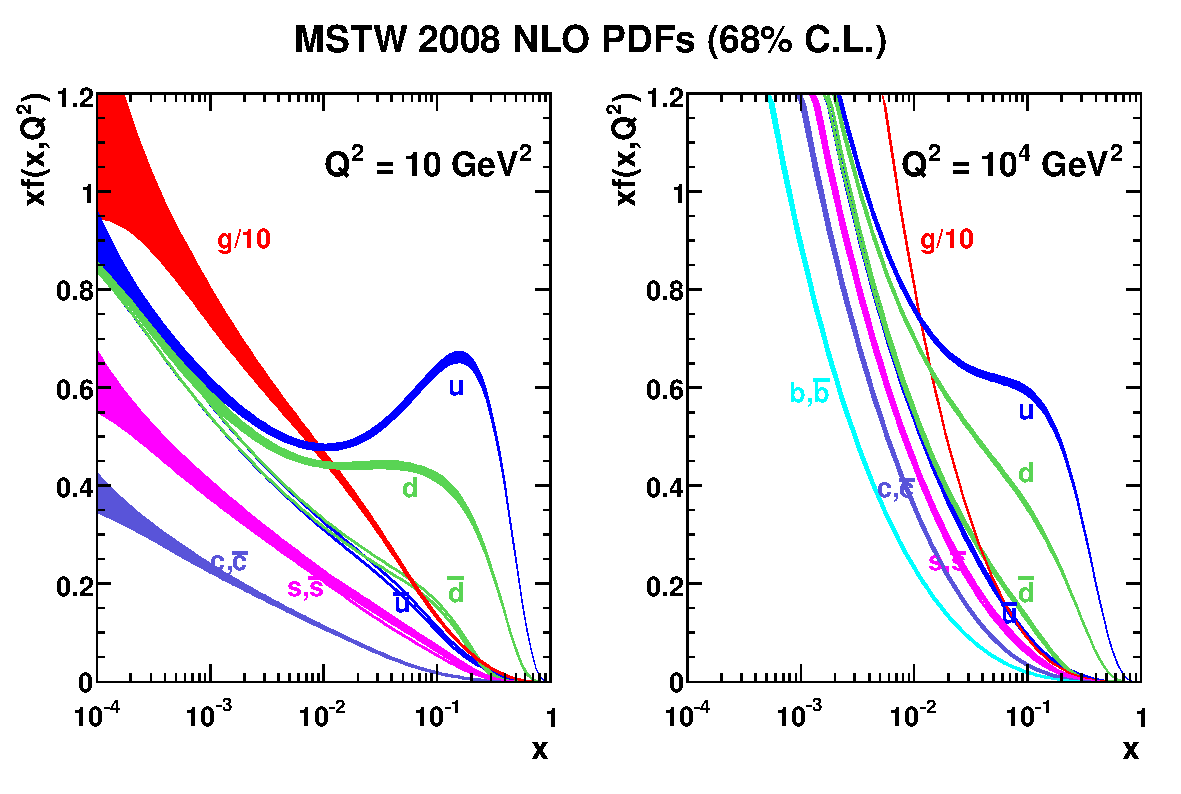
\includegraphics[width=0.9\textwidth]{images/pdfs.pdf}
  \caption{Typical momentum fraction distributions of partons inside the proton at a factorisation scale of \(Q^2 = 10\,\text{GeV}^2\) (left) and \(Q^2 = 10\,\text{GeV}^2\) (right). The plot shows the gluon and the first two generations of quarks, including valence $up$-quark and $down$-quark components~\cite{Martin_2009}.}
  \label{fig:pdfs}
\end{figure}

\subsubsection*{Parton-parton scattering}
\label{subsubsec:proton}
From these principles, the production cross-sections for the processes that unfold at hadron colliders can be factorized into two contributions. The PDFs describe the colliding partons $a$, $b$, within the colliding hadrons $H_{A}$, $H_{B}$. In the collision, the hard scattering process of interest corresponds to the short-distance interaction between both partons, each carrying a fraction of the parent hadrons's momentum. These interactions are characterised by a large momentum transfer and are described within the framework of perturbative QCD. However, the collision environment also includes soft interactions with low momentum transfer, collectively referred to as the underlying event (UE), which encompasses remnants of the hadron-hadron system as well as potential multi-parton interactions (MPI), which are cases where more than one partonic interaction occurs within a single event.

Radiative processes such as Bremsstrahlung are inherent to high-energy collisions due to the acceleration of colour and electric charges. Initial State Radiation (ISR) arises from the incoming partons before the hard interaction, while Final State Radiation (FSR) originates from the outgoing partons. Following the hard interaction, partons undergo hadronisation, a non-perturbative QCD process in which coloured partons are confined into colour-singlet hadrons. These hadrons are typically collimated into jets, observable in the detector.

Hence, the total production cross-section for a given final state $X$ in a $pp$ collision is obtained via the factorisation theorem~\cite{fact_them,collins2004factorizationhardprocessesqcd}:
\begin{equation}
\sigma_{AB \to X} = \sum_{a,b} \int \mathrm{d}x_a \, \mathrm{d}x_b \, f_{a/A}(x_a, \mu_F^2) \, f_{b/B}(x_b, \mu_F^2) \, \hat{\sigma}_{ab \to X}(\hat{s}, \mu_R^2),
\end{equation}
where $f_{a/A}$ and $f_{b/B}$ are the PDFs containing the non-perturbative component of the soft interaction, $\mu_F$ is the factorisation scale, and $\mu_R$ the renormalisation scale associated with the running of $\alpha_s$. The partonic production cross-section $\hat{\sigma}$ is computed as a perturbative expansion in $\alpha_s(\mu_R)$:
\begin{equation}
\hat{\sigma}_{ab \to X} = \hat{\sigma}_0 + \alpha_s(\mu_R^2)\, \hat{\sigma}_1 + \alpha_s^2(\mu_R^2)\, \hat{\sigma}_2 + \cdots.
\label{running}
\end{equation}

While leading order (LO) calculations offer basic estimates, they suffer from large theoretical uncertainties due to strong dependence on $\mu_F$ and $\mu_R$. Higher-order corrections at next-to leading order (NLO) or next-to-next-to leading order (NNLO) reduce this dependence and yield more accurate predictions. The impact of these corrections is often quantified via the $K$-factor, defined as the ratio of the production cross-sections computed at higher orders in QCD with respect to the LO cross-section.

%----------------------------------------------
\subsection{Electroweak Theory and Gauge Unification}
\label{subsec:ew_theory}
%----------------------------------------------

The electroweak (EW) theory unifies the weak and electromagnetic interactions within a single gauge framework. It is formulated as a non-Abelian gauge theory based on the symmetry group $SU(2)_L \times U(1)_Y$, where $SU(2)_L$ accounts for weak isospin and $U(1)_Y$ for weak hypercharge. The theory was developed independently by Glashow, Weinberg, and Salam~\cite{Glashow,Weinberg,Salam}, and constitutes a central component of the SM. The electroweak Lagrangian can be written as:

\begin{equation}
\begin{split}
\mathcal{L}_{\text{EW}} = 
&\sum_{flavours} i(\bar{L}\gamma^\mu D_\mu L +\bar{Q}\gamma^\mu D_\mu Q + \bar{l}_{R}\gamma^\mu D_\mu l_{R} + \bar{u}_{R}\gamma^\mu D_\mu u_{R} + \bar{d}_{R}\gamma^\mu D_\mu d_{R}) \\
&- \frac{1}{4} W_{\mu\nu}^a W^{a\,\mu\nu} - \frac{1}{4} B_{\mu\nu} B^{\mu\nu}
\end{split}
\label{eq:ew_lagrangian}
\end{equation}

The gauge fields associated with $SU(2)_L$ are denoted by $\vec{W}_\mu = (W_\mu^1, W_\mu^2, W_\mu^3)$, while the gauge field corresponding to $U(1)_Y$ is $B_\mu$. The corresponding gauge couplings are $g$ and $g'$, respectively. The covariant derivative acting on fermion fields is given by:
\begin{equation}
D_\mu = \partial_\mu - i \, g \, \frac{\vec{\tau}}{2} \cdot \vec{W}_\mu - i \, g' \, \frac{Y}{2} B_\mu,
\end{equation}
where $\vec{\tau}$ are the Pauli matrices and $Y$ is the weak hypercharge of the field.

Left-handed fermions are arranged in $SU(2)_L$ doublets, while right-handed fermions transform as singlets. For instance, the first-generation leptons are written as:
\begin{equation}
L_e =
\begin{pmatrix}
\nu_e \\
e
\end{pmatrix}_L, \qquad e_R,
\end{equation}
with $L_e$ transforming as a doublet under $SU(2)_L$ and $e_R$ as a singlet. It similarly applies to left-handed quark doublets, $Q$, and singlets, $u$ and $d$. The weak hypercharges are assigned such that the electric charge $Q$ of each field is given by the Gell-Mann–Nishijima relation:
\begin{equation}
Q = T_3 + \frac{Y}{2},
\end{equation}
where $T_3$ is the third component of weak isospin.

The kinetic term of the gauge fields is given by:
\begin{equation}
\mathcal{L}_{\text{gauge}} = -\frac{1}{4} \, \vec{W}_{\mu\nu} \cdot \vec{W}^{\mu\nu} - \frac{1}{4} \, B_{\mu\nu} B^{\mu\nu},
\end{equation}
where the field strength tensors are defined as:
\begin{align}
W_{\mu\nu}^i &= \partial_\mu W_\nu^i - \partial_\nu W_\mu^i + g \, \epsilon^{ijk} W_\mu^j W_\nu^k, \\
B_{\mu\nu} &= \partial_\mu B_\nu - \partial_\nu B_\mu.
\end{align}

Fermion interactions with the gauge bosons arise from the kinetic term of the fermion fields:
\begin{equation}
\mathcal{L}_{\text{fermion}} = \sum_{\psi} \bar{\psi} \, i \slashed{D} \, \psi,
\end{equation}
leading to charged and neutral current interactions. The charged currents couple only to left-handed fermions via $W^\pm$ bosons (linear combinations of $W^1$ and $W^2$), while neutral currents arise from couplings to $W^3$ and $B$.

At this stage, all gauge bosons and fermions are massless. Mass terms are forbidden by gauge invariance, and it is only through spontaneous symmetry breaking that physical masses are generated, as discussed in Section~\ref{subsec:higgs_mech}. Additionally, the structure of the theory prior to breaking ensures parity violation in weak interactions due to the chiral nature of the $SU(2)_L$ coupling.

This unbroken EW theory thus describes the fundamental structure of weak and electromagnetic interactions prior to the introduction of the Higgs field, which provides masses to the gauge bosons and fermions while preserving gauge invariance through the Higgs mechanism.

%----------------------------------------------
\subsection{Spontaneous Symmetry Breaking and the Higgs Mechanism}
\label{subsec:higgs_mech}
%----------------------------------------------

In order to generate the mass of weak vector bosons and fermions while preserving renormalizability and unitarity, the SM introduces a Spontaneous Symmetry Breaking mechanism in the electroweak theory. 
This mechanism is referred to as the Brout–Englert–Higgs (BEH) mechanism~\cite{Brout,HiggsSpontan}, and it introduces a complex scalar field doublet $\phi$ with hypercharge $Y=+1$, whose dynamics are governed by the gauge-invariant Lagrangian:
\begin{equation}
\mathcal{L}_\phi = (D_\mu \phi)^\dagger(D^\mu \phi) - V(\phi),
\end{equation}
where $V(\phi)$ is the scalar potential:
\begin{equation}
V(\phi) = \mu^2 \phi^\dagger \phi + \lambda(\phi^\dagger \phi)^2,
\label{eq:higgs_potential}
\end{equation}
with $\lambda > 0$ ensuring the potential is bounded from below. The sign of $\mu^2$ determines the nature of the vacuum: for $\mu^2 > 0$, the potential has a single minimum at $\phi = 0$, preserving the gauge symmetry. However, for $\mu^2 < 0$, the potential takes the shape of a “Mexican hat”, as illustrated in Figure~\ref{fig:mexican_hat}, with a continuous set of degenerate minima.

Since the Lagrangian is gauge invariant, the Higgs field can be described using an exponential decomposition:
\begin{equation}
\phi(x) = \frac{1}{\sqrt{2}} \, e^{i \tau_{a} \theta^a(x)/f} \begin{pmatrix}
0 \\
\rho(x)
\end{pmatrix},
\label{eq:higgs_param}
\end{equation}
where $\theta^a(x)$ and $\rho(x)$ are real fields, $\tau_{a}$ are the SU(2) generators\footnote{Elements of the group that generate the group when combined with themselves using the group's operations}, and $f$ is a normalisation constant.

One of the degenerate minima can be chosen without loss of generality as:
\begin{equation}
\langle \phi \rangle = \frac{1}{\sqrt{2}} \begin{pmatrix}
0 \\
v
\end{pmatrix},
\end{equation}
which spontaneously breaks the $SU(2)_L \times U(1)_Y$ gauge symmetry down to the electromagnetic subgroup $U(1)_{\text{EM}}$.

\begin{figure}[htbp]
  \centering
  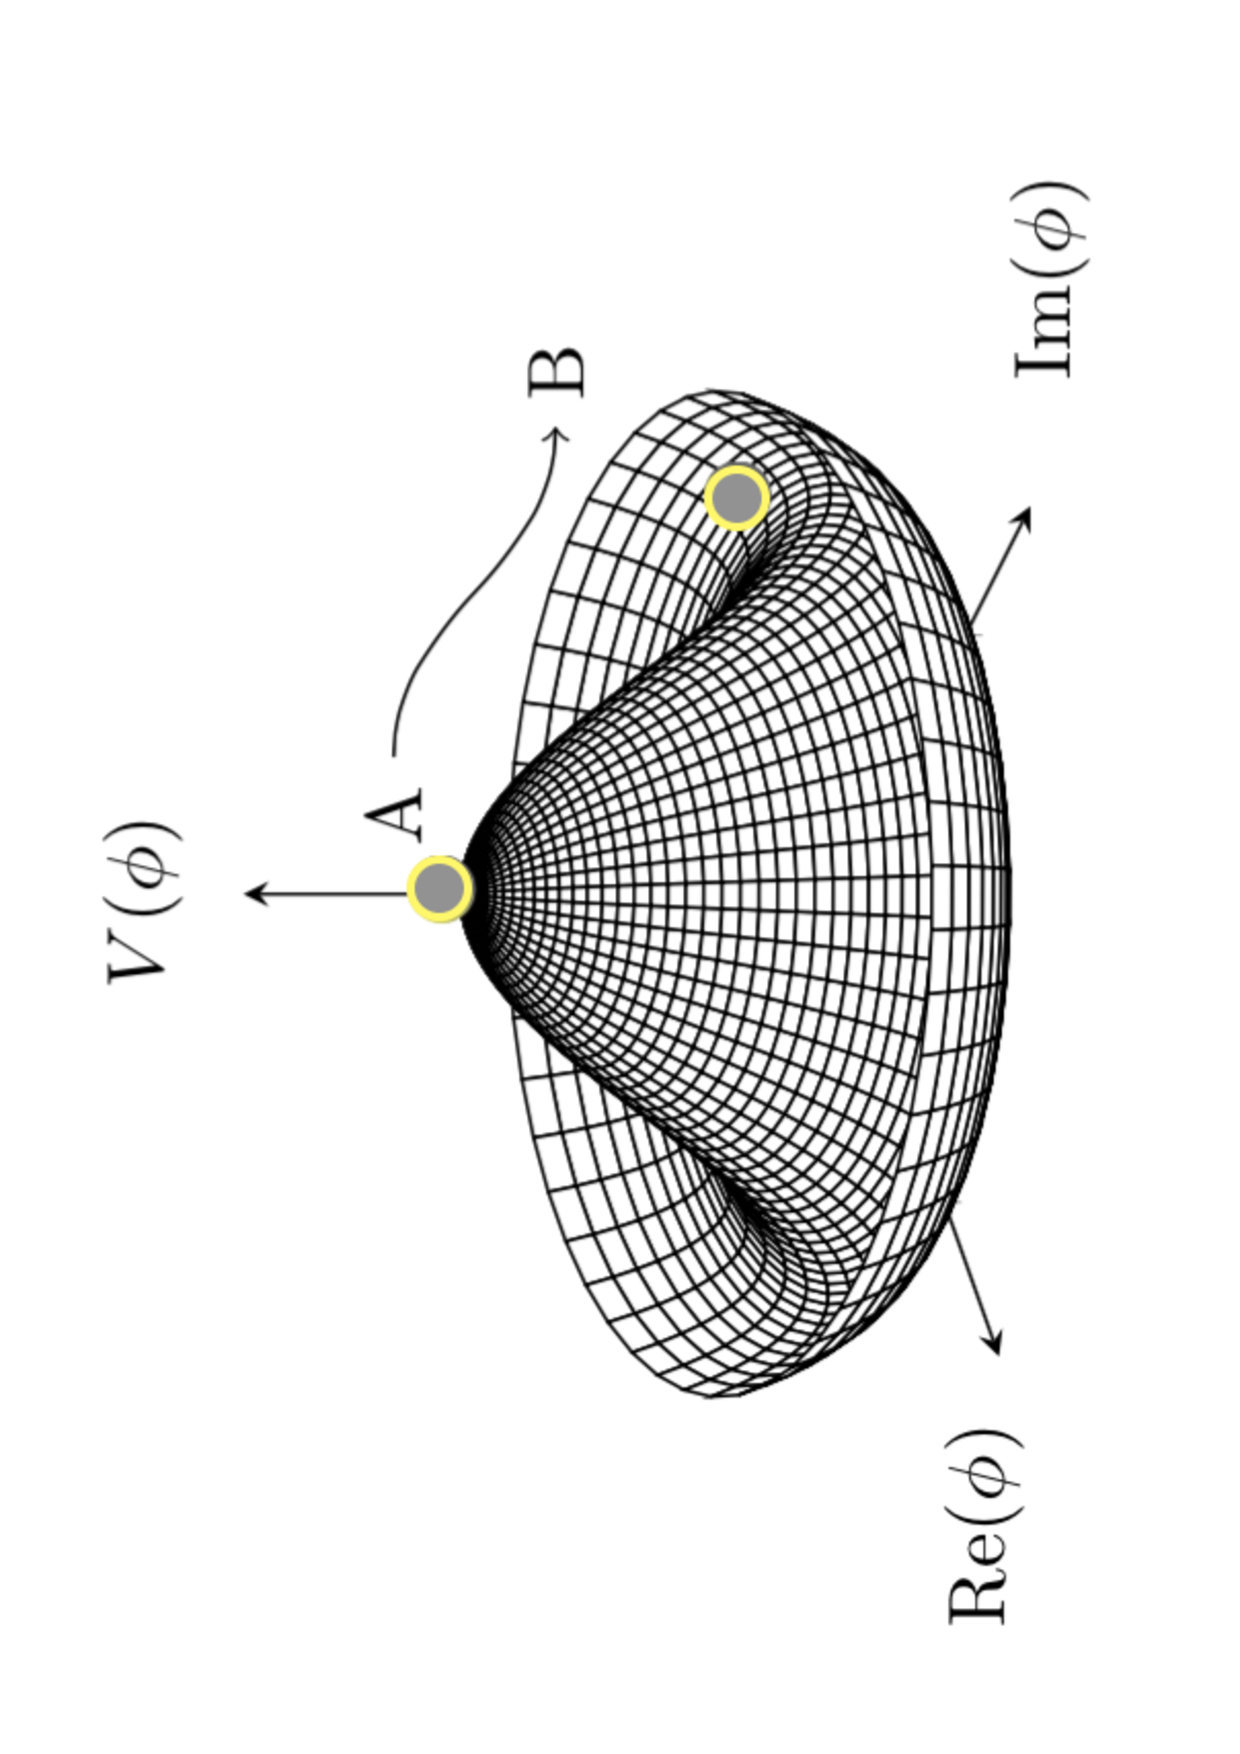
\includegraphics[angle=-90,width=0.7\textwidth]{images/mexican_hat.pdf}
  \caption{Illustration of the shape of the Higgs complex scalar potential with vacuum expectation value $v$. The symmetry is spontaneously broken when a singular ground state is chosen (A $\rightarrow$ B).}
  \label{fig:mexican_hat}
\end{figure}

The simplest way to expand the Higgs field is to keep the minimum number of degrees of freedom, so replacing $v\rightarrow v+h(x)$ in the previous equation and substituing in the potential Lagrangian (Eq.~\ref{eq:higgs_potential}): 
\begin{equation}
\begin{split}
\mathcal{L}_{H} = 
&\frac{1}{2}(\partial_{\mu}h)(\partial^{\mu}h) + \frac{1}{2}(2\mu^2)h^2\\  
& + \frac{1}{2}\frac{g^2_{W}v^2}{4}(W_{\mu}^1W^{1\mu}+W_{\mu}^2W^{2\mu})\\
& +\frac{1}{8}v^2(g_{W}W^{3\mu}-g_{B}B^{\mu})\\ 
& + \mathcal{O}(h^2)
\end{split} 
\label{eq:ew_broken}
\end{equation}

This expression contains quadratic terms interpreted as the mass terms of the particles associated to the fields. Since gauge boson terms here are not linearly independent, they cannot be interpreted as observables. Physical bosons can be obtained diagonalizing this sector, resulting in:
\begin{align}
W^\pm_\mu &= \frac{1}{\sqrt{2}} \left( W^1_\mu \mp i W^2_\mu \right), \\
Z_\mu &= \cos\theta_W W^3_\mu - \sin\theta_W B_\mu, \\
A_\mu &= \sin\theta_W W^3_\mu + \cos\theta_W B_\mu,
\end{align}
where $\theta_W$ is the weak mixing angle defined by $\tan \theta_W = g_B /g_W$.
Using these definitions, the corresponding masses of the gauge bosons can be obtained from the Lagrangian as follows:
\begin{align}
m^{\pm}_W &= \frac{1}{2} g v, \\
m_Z &= \frac{1}{2} \sqrt{g^2 + g'^2} \, v, \\
m_\gamma &= 0,
\end{align}
where $v = 246 \text{  GeV}$ is the Higgs field vacuum expectation value and $g$ is the weak isospin coupling constant. 
This mechanism results in two massive vector bosons $W^{\pm}$ which corresponds to the weak charged current, and other massive boson $Z$, carrier of the neutral weak current. It also remains a massless gauge boson, $A_{\mu}$, which corresponds to the photon and is consistent with the unbroken QED symmetry $U(1)$.

From Eq.~\ref{eq:ew_broken}, the mass term for the scalar field $H$ turns to be:
\begin{equation}
m_H^2 = 2 \mu^2,
\end{equation}
where it depends on the free parameter $\mu^2$, that can be experimentally measured, and it has been found to be close to $125$~GeV.
Actually, this Lagrangian can also be expressed in the following way after the spontaneous symmetry breaking: 
\begin{align}
\mathcal{L}_{H} &= m_W^2 W^-_{\mu} W^{+\mu} \left( 1 + \frac{h}{v} \right)^2
+ \frac{1}{2} m_Z^2 Z_{\mu} Z^{\mu} \left( 1 + \frac{h}{v} \right)^2 \notag \\
&\quad + \frac{1}{2} (\partial_{\mu} h)^2 - V(h).
\label{allterms}
\end{align}
with
\begin{equation}
    V(h) = -\frac{\mu^{4}}{4\lambda} - \mu^2h^2 + \lambda v h^3 + \frac{\lambda}{4}h^4
\label{hcoupl}
\end{equation}
where apart from the aforementioned mass term for the Higgs field, this equation also contains the Higgs self-interaction terms $h^3$ and $h^4$. 

Moreover, the BEH mechanism can also be used to provide mass terms for the fermions preserving the gauge invariance of the theory.
Adding the Yukawa terms~\cite{Peskin} describing fermion couplings to the Higgs field into the EW Lagrangian, one gets:
\begin{equation}
\mathcal{L}_{\text{Yukawa}} = 
\sum_{\text{flavours}} \left( 
- \lambda_\ell \, \bar{L} \phi \ell_R 
- \lambda_d \, \bar{Q} \phi d_R 
- \lambda_u \, \epsilon^{ab} \, \bar{Q}_a \phi_b^{\dagger} u_R 
+ \text{h.c.} 
\right)
\end{equation}
where $\lambda_{e}$, $\lambda_{d}$ and $\lambda_{u}$ are arbitrary parameters and $\epsilon^{ab}$ is the two dimensional total anti-symmetric tensor with $\epsilon^{12}=1$. After symmetry breaking we get the following mass terms for the fermion fields after proper diagonialization: 
\begin{equation}
m_{\ell}=\lambda_{\ell}\frac{v}{\sqrt{2}}, \ m_{d}=\lambda_{d}\frac{v}{\sqrt{2}}, \ m_{u}=\lambda_{u}\frac{v}{\sqrt{2}},
\end{equation}
from where the Yukawa coupling strength of fermions to the Higgs field can be defined as
\begin{equation}
\label{yukawa}
y_{f}=\sqrt{2}\frac{m_{f}}{v}
\end{equation}
Moreover, these fermion mass eigenstates and the weak eigenstates are related via the $3\times3$ unitary Cabibbo-Kobayashi-Maskawa (CKM) matrix, $V_{CKM}$,
\begin{equation}
\begin{pmatrix}
d^0 \\
s^0 \\
b^0
\end{pmatrix}
= V_{\text{CKM}}
\begin{pmatrix}
d \\
s \\
b
\end{pmatrix}
=\begin{pmatrix}
V_{ud} & V_{us} & V_{ub} \\
V_{cd} & V_{cs} & V_{cb} \\
V_{td} & V_{ts} & V_{tb}
\end{pmatrix}
\begin{pmatrix}
d \\
s \\
b
\end{pmatrix},
\end{equation}
where the off-diagonal elements cause flavour changing weak charged current interactions of quarks with their transition probabilities being proportional to $|V_{nm}|^2$.

%++++++++++++++++++++++++++++++++++++++++++++++
\section{Success and limitations of the SM}
\label{sec:BSM}
%++++++++++++++++++++++++++++++++++++++++++++++
After integrating all the essential elements forming the SM, the theory is characterized by 19 undetermined parameters:
\begin{itemize}
  \item a total of nine Yukawa couplings corresponding to the three charged leptons and six quarks;
  \item three gauge coupling constants governing the strengths of the interactions: \( g_s \), \( g \), and \( g' \);
  \item two parameters characterizing the Higgs potential: the vacuum expectation value \(\nu\) and the Higgs boson mass \(m_H\);
  \item four resulting mixing angles defining the structure of the CKM matrix;
  \item a single strong $CP$-violating phase \(\theta_{CP}\), which is conventionally assumed to be zero, implying the absence of $CP$ violation in strong interactions.
\end{itemize}
Despite being defined by 19 free parameters, the SM has demonstrated extraordinary predictive power, with theoretical predictions consistently matching experimental results over several decades. This success is exemplified in Figure~\ref{fig:totalxsect}, which presents the production cross-sections measured by the ATLAS experiment for a variety of processes occurring across multiple orders of magnitude.
\begin{figure}[htbp]
  \centering
  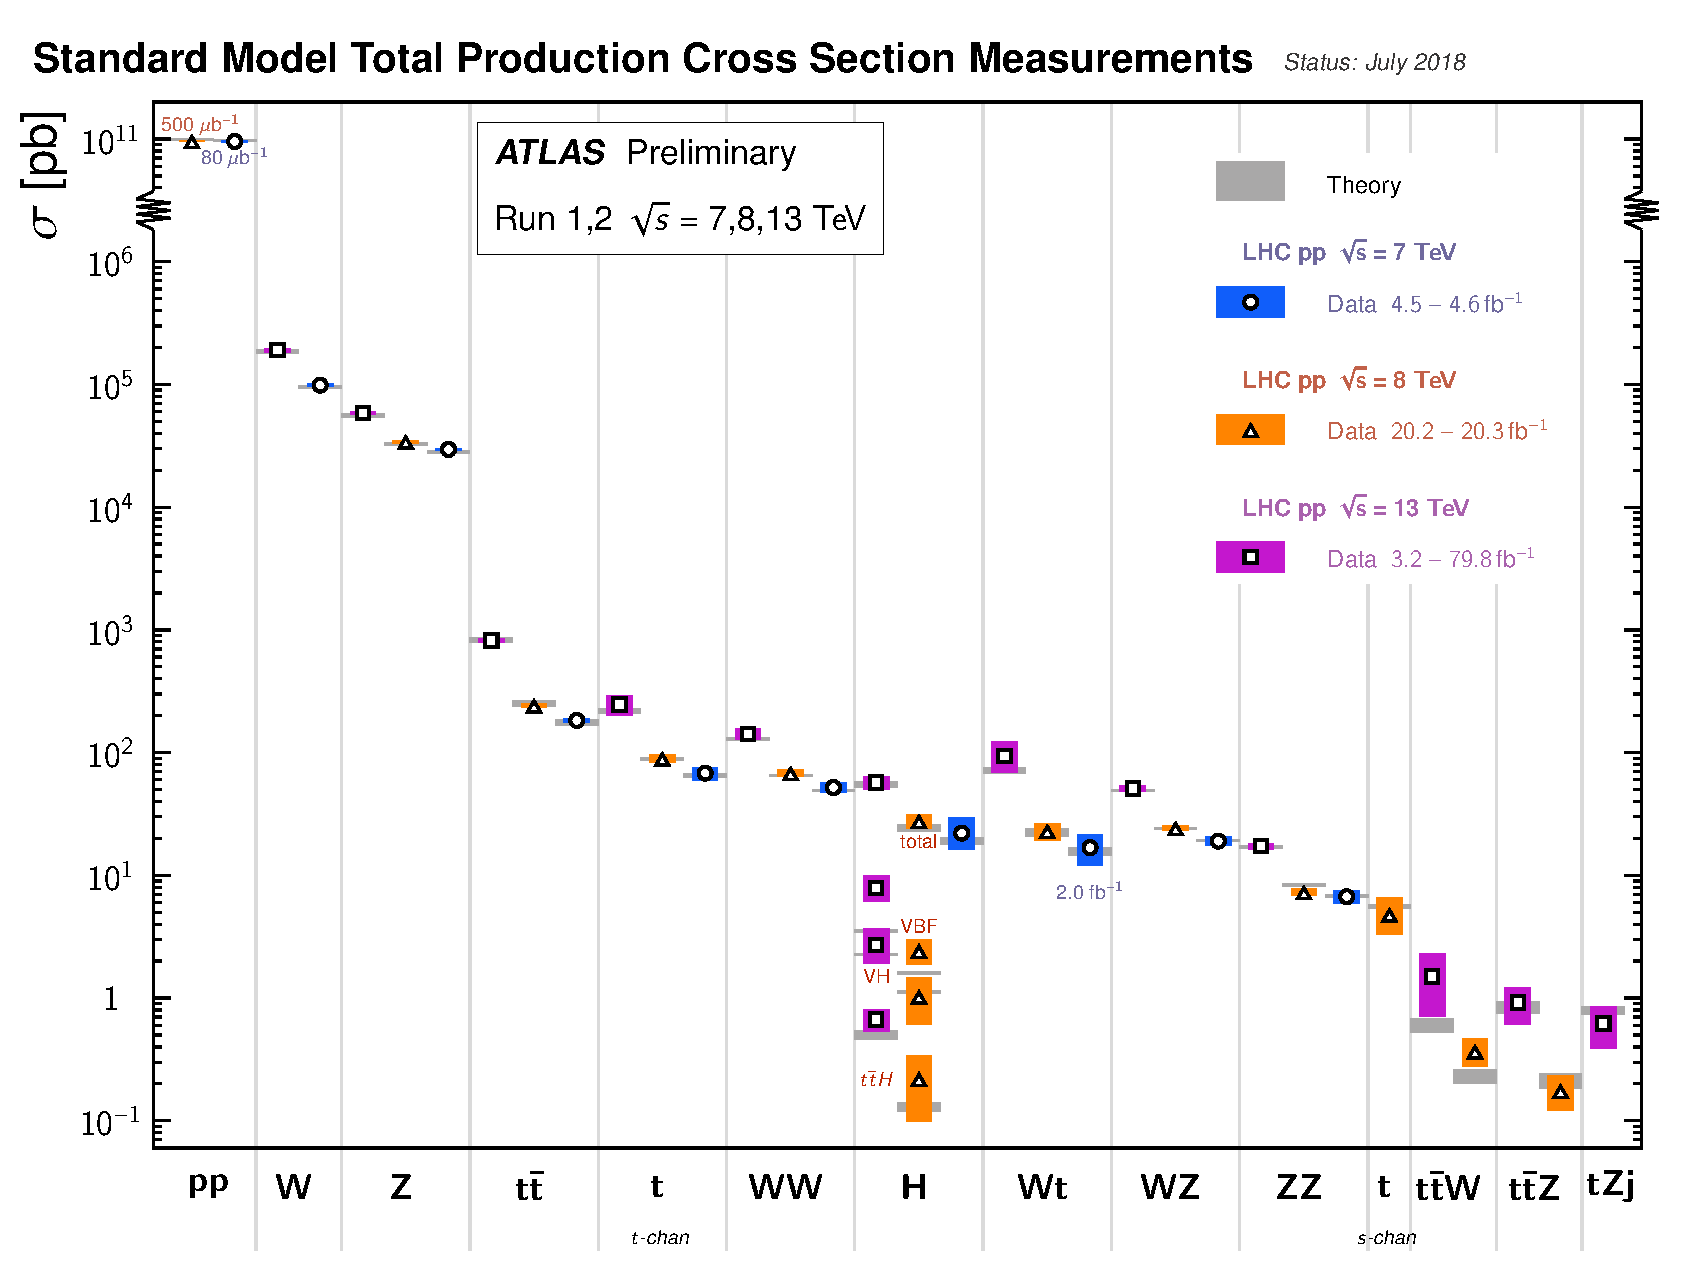
\includegraphics[width=0.8\textwidth]{images/totalxsect.pdf}
  \caption{Summary of several SM total production cross-section measurements, compared to the corresponding theoretical expectations. All theoretical expectations were calculated at NLO or higher~\cite{ATL-PHYS-PUB-2024-011}.}
  \label{fig:totalxsect}
\end{figure}

Despite its remarkable success, the SM is not considered a complete theory of fundamental interactions. Some of the most relevant issues not addressed by this theory are:
\subsubsection*{Dark Matter}

Astrophysical and cosmological observations provide compelling evidence for the existence of dark matter (DM), a form of non-luminous matter not accounted for in the SM. Measurements of galactic rotation curves, gravitational lensing in galaxy clusters (e.g., the Bullet Cluster~\cite{Clowe_2006}), and the cosmic microwave background anisotropies consistently indicate that approximately 85\% of the matter content of the universe is non-baryonic~\cite{Planck}. While several extensions of the SM propose viable DM candidates, such as weakly interacting massive particles or axions, the SM itself does not provide a suitable particle to explain these phenomena.

\subsubsection*{Neutrino Masses and Oscillations}

Experimental evidence from solar, atmospheric, reactor, and accelerator neutrino experiments has firmly established that neutrinos undergo flavor oscillations, implying they have non-zero masses and mixings~\cite{PhysRevD.98.030001}. This observation requires the existence of mass terms beyond the SM original framework, which assumes massless neutrinos. Mechanisms such as the seesaw model, introducing right-handed neutrinos or Majorana mass terms, are common in theories beyond the SM (BSM), but are not present in its minimal formulation.

\subsubsection*{Matter-Antimatter Asymmetry}

The observed universe is dominated by matter over antimatter, a phenomenon known as baryon asymmetry. While the SM includes a source of $CP$ violation through the complex phase in the CKM matrix, it is insufficient to account for the observed phenomena. Additional sources of $CP$ violation and new physics at high energy scales are required to explain this asymmetry.

\subsubsection*{Hierarchy Problem}

The mass of the Higgs boson receives large quantum corrections proportional to the square of the energy cutoff scale of the theory. Stabilizing the Higgs boson mass at the electroweak scale without unnatural fine-tuning requires a mechanism to cancel these divergences~\cite{Weinberg:1975gm,Gildener:1976ai,Weinberg:1979bn,Susskind:1978ms}. Supersymmetry~\cite{Dimopoulos:1981zb,Witten:1981nf,Dine:1981za,Dimopoulos:1981au,Sakai:1981gr,Kaul:1981hi}, composite Higgs models, and extra-dimensional theories have been proposed as potential solutions, but no evidence of such physics has been observed.

\subsubsection*{Gravity and the Lack of Unification}

The SM does not incorporate gravity, which is described by General Relativity. Moreover, the gauge couplings of the SM do not unify at a single energy scale, unless new physics is introduced. A complete theory of fundamental interactions would require a quantum theory of gravity and a framework capable of unifying all known forces, such as string theory or grand unified theories (GUTs).

\subsubsection*{Vacuum Stability and the Top-Quark Yukawa Coupling}

The stability of the EW vacuum is governed by the behaviour of the Higgs field self-coupling $\lambda$ under renormalization group (RG) evolution. In this context, the $\beta$-function encodes the scale dependence of $\lambda$ as
$\beta_\lambda \equiv d\lambda/ d \ln Q$, and determines whether the scalar potential remains stable at very high energies. At tree level, the potential in Eq.~\ref{hcoupl} is stable provided that $\lambda>0$. However, radiative corrections can alter this behaviour, driving $\lambda(Q)$ to negative values for sufficiently large $Q$. In such a case, the EW vacuum is only metastable, with a deeper minimum appearing at large field values.

Among all SM parameters, the Higgs boson mass $m_H$, the strong coupling $\alpha_s$, and especially the top-quark mass $m_t$ play the most significant roles. The value of $m_H$ sets the boundary condition for $\lambda$ at the electroweak scale, while $m_t$ determines the size of the top-quark Yukawa coupling $y_t$. Being the largest Yukawa coupling, $y_t$ provides a dominant and negative contribution to $\beta_\lambda$, effectively lowering $\lambda$ at high scales. As a consequence, the question of whether the SM vacuum is stable, metastable, or unstable is extremely sensitive to the precise value of $y_t$. Even small shifts in $m_t$ can qualitatively change the fate of the vacuum. This stability issue arises in the absence of new physics at higher energies, whereas possible effects from BSM physics could alter the running of $\lambda$ and prevent the development of such an instability.

This behaviour is illustrated in Figure~\ref{fig:vacuum_stability}. The left panel shows the full phase diagram of the SM in the $(m_t,m_H)$ plane, with regions of absolute stability, metastability, instability, and non-perturbativity. The right panel zooms into the phenomenologically relevant region around the experimentally measured values of $m_t$ and $m_H$. The figure highlights that these values lie very close to the critical boundary separating stability and metastability, suggesting that the Universe likely resides in a long-lived but metastable vacuum~\cite{Degrassi_2012}.

The importance of these considerations goes beyond a purely theoretical curiosity. Since the top-quark Yukawa coupling is the key player in determining the high-scale behaviour of $\lambda$, precision measurements of processes such as associated $t\bar{t}H$ production are essential. They not only test the SM at the electroweak scale but also probe the structure of the Higgs potential up to the Planck scale.

\begin{figure}[htbp]
    \centering
    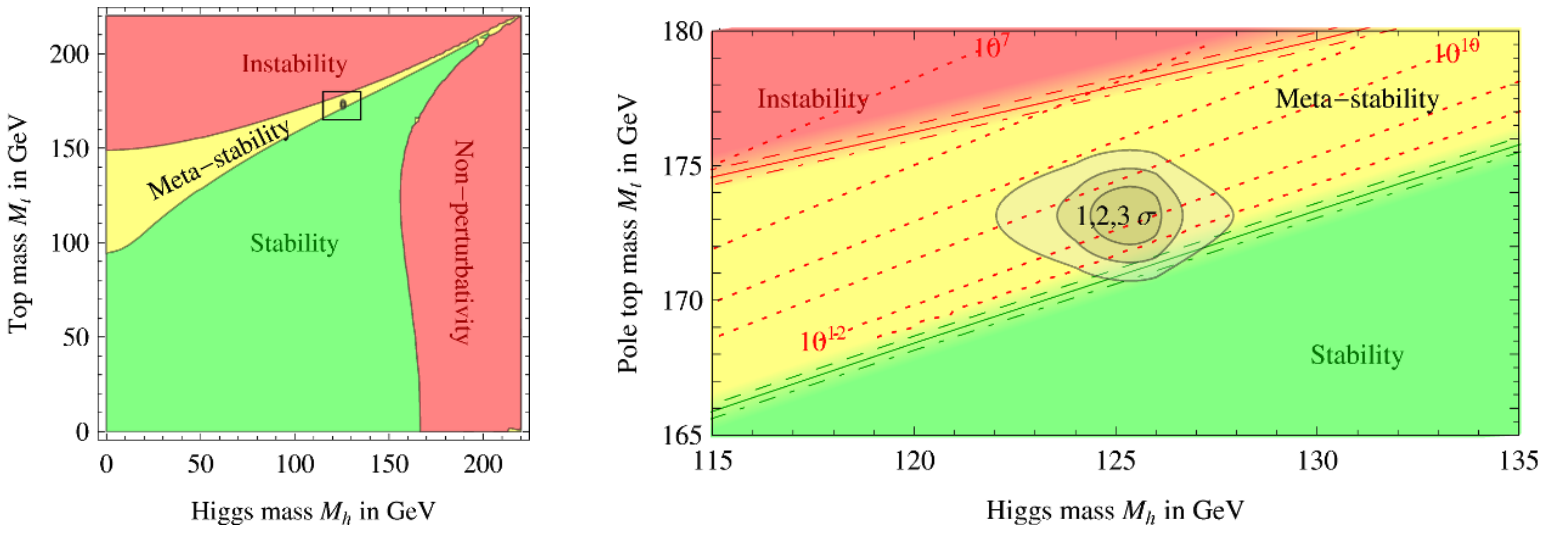
\includegraphics[width=0.9\textwidth]{images/vacuum.png}
    \caption{
        Regions of absolute stability, metastability and instability of the SM vacuum in the $(m_t, m_H)$ plane. 
        Left: full phase diagram including the region of non-perturbativity at large Higgs mass. 
        Right: zoom into the region of phenomenological interest, around the experimentally measured values of $m_t$ and $m_H$, where the Universe appears to lie close to the boundary between stability and metastability. 
        Adapted from Ref.~\cite{Degrassi_2012}.
    }
    \label{fig:vacuum_stability}
\end{figure}
%++++++++++++++++++++++++++++++++++++++++++++++
\section{Phenomenology of the Top Quark and the Higgs Boson at the LHC}
\label{sec:top_higgs_lhc}
%++++++++++++++++++++++++++++++++++++++++++++++
The top quark and the Higgs boson play a central role in the SM and in the exploration of physics beyond it. Their large masses, unique interactions, and profound implications for EWSB and vacuum stability make them particularly interesting from both theoretical and experimental perspectives. 

%xxxxxxxxxxxxxxxxxxxxxxxxxxxxxxxxxxxxxxxxxxxxxxxxxxxxxx
\subsection{The Top quark}
\label{sec:top_quark}
%xxxxxxxxxxxxxxxxxxxxxxxxxxxxxxxxxxxxxxxxxxxxxxxxxxxxxx

The top quark, initially proposed by Kobayashi and Maskawa in 1973~\cite{10.1143/PTP.49.652} and discovered at the Tevatron in 1995~\cite{PhysRevLett.74.2626,PhysRevLett.74.2632}, is the heaviest known elementary particle, with a mass of about $173$~GeV. Its extremely short lifetime causes it to decay before hadronization can occur, predominantly into a $W$ boson and a $b$ quark. Although decays into other down-type quarks are possible in principle, they are strongly suppressed by the structure of the CKM matrix and therefore negligible. Owing to its large mass, the top quark also possesses a Yukawa coupling close to unity.

\subsubsection*{Top quark production}
\label{subsec:top_quark_prod}
At hadron colliders such as the LHC, the top quark production mostly ocurrs in pairs ($t\bar{t}$) through the strong interaction. At LO, the two leading subprocesses are gluon-gluon fusion (ggF) and $q\bar{q}$ annihilation, as represented in Figure~\ref{fig:tt-production}. Gluon fusion accounts for roughly $90\%$ of the total $t\bar{t}$ production cross-section at a centre-of-mass energy of 13 TeV.
\begin{figure}[htbp]
    \centering
    \subfloat[]{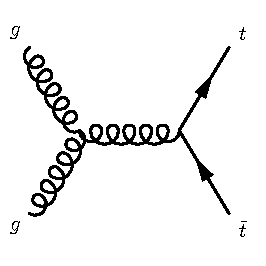
\includegraphics[width=0.3\textwidth]{feyn_gg_ttbar_1.pdf}}
    \hfill
    \subfloat[]{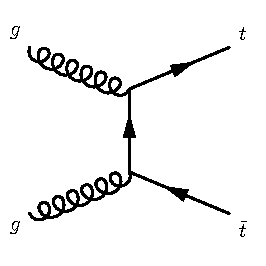
\includegraphics[width=0.3\textwidth]{feyn_gg_ttbar_2.pdf}}
    \hfill
    \subfloat[]{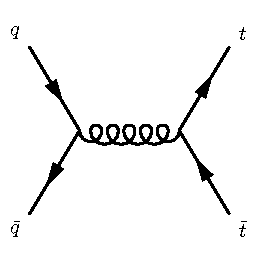
\includegraphics[width=0.3\textwidth]{feyn_qq_ttbar.pdf}}
    \caption{Leading-order Feynman diagrams contributing to top quark pair production in hadron colliders: (a) and (b) gluon-gluon fusion, which is the dominant process at the LHC, and (c) quark-antiquark annihilation, which dominates at lower center-of-mass energies such as at the Tevatron.}
    \label{fig:tt-production}
\end{figure}


Nevertheless, top quarks can also be produced singly via the electroweak interaction, either alone or in association with other particles. Single-top has a much smaller production cross-section, but processes like $tW$ or \tH encapsulate important complementary information.
Among all of them, \tH and \ttH play a central role in this thesis by forming the signal processes that are discussed in the last chapters of the thesis. They will be futher covered in more detail at the end of this chapter.

\subsubsection*{Top-antitop system decay}
\label{subsec:top_quark_decay}

Given that the top quark decays nearly the $100\%$ of cases as $t\rightarrow Wb$, the properties of $t\bar{t}$ final states mainly depend on how the $W$ boson decays, as it is shown in Figure~\ref{fig:diagram-top}.
\begin{figure}[htbp]
    \centering
    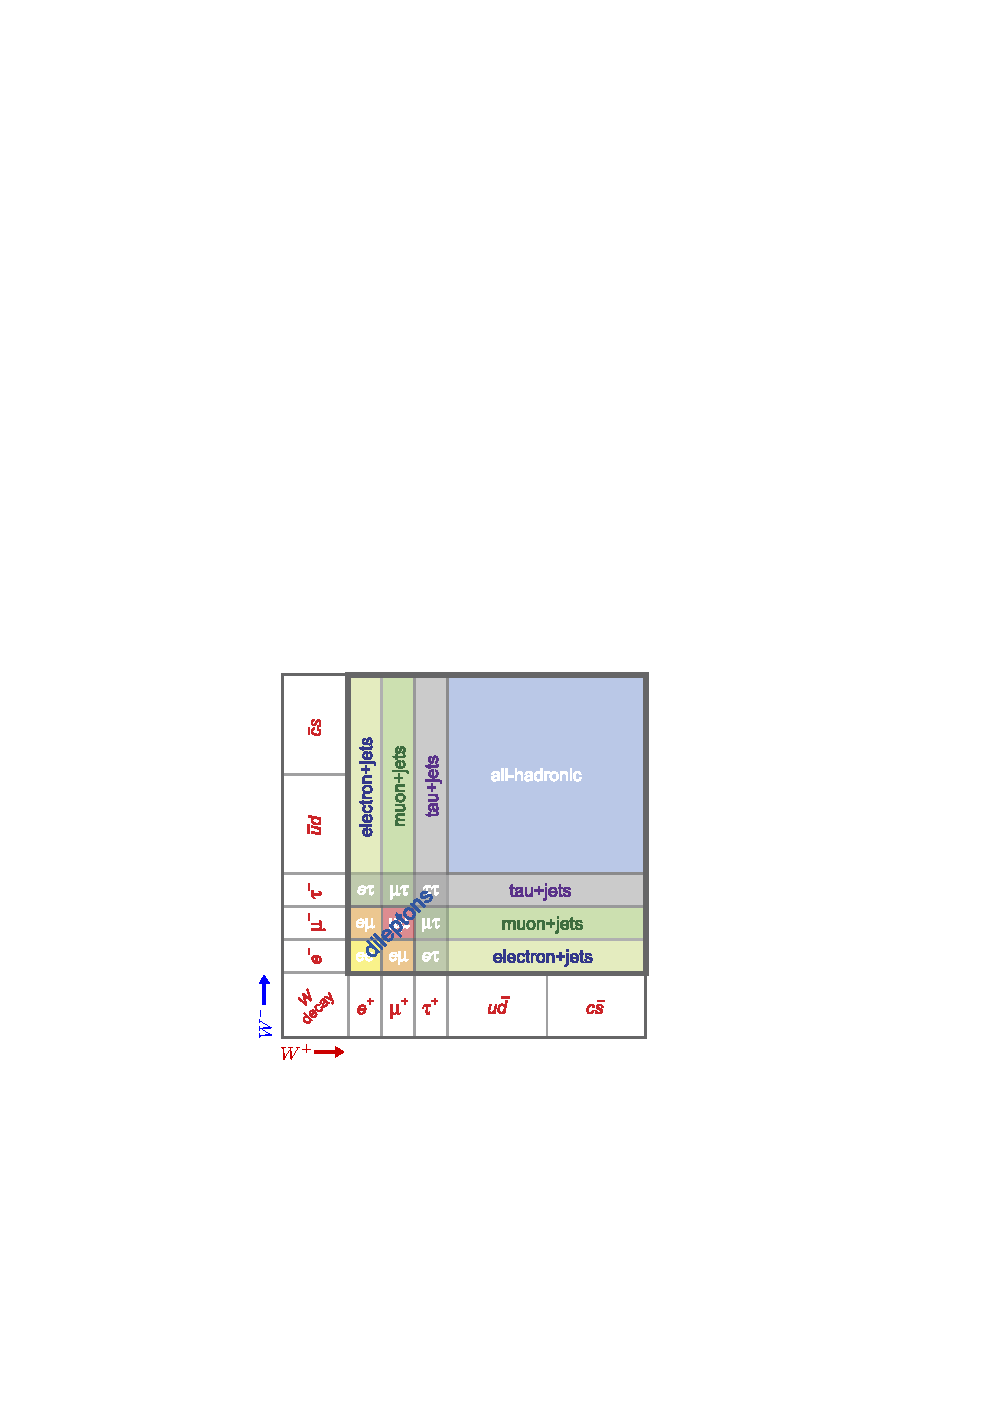
\includegraphics[width=0.5\textwidth]{tt_decay_channels.pdf}
    \caption{Classification of $t\bar{t}$ decay channels based on the $W$ decay modes~\cite{Lannon_2012}.}
    \label{fig:diagram-top}
\end{figure}

The fully hadronic final state corresponds to the case where both $W$ bosons decay into quark-antiquark pairs. This is the most frequent decay mode. An smaller fraction of events corresponds to the semileptonic final state, in which one of the bosons decays hadronically, while the other decays leptonically producing a charged lepton and a neutrino. In the case of the dileptonic final state, both $W$ bosons decay into leptons.

The table in Figure~\ref{fig:diagram-top} considers $\tau$-leptons within the general category of leptons. However, in the context of physics analysis, it is common for the term ``leptonic decay'' to be used only to refer to decays into ``light leptons'', i.e. electrons and muons, including those from the decay of $\tau$-leptons. For experimental reasons, hadronic decays of $\tau$-leptons are treated differently, as discussed in Section~\ref{sec:ttH}.

%xxxxxxxxxxxxxxxxxxxxxxxxxxxxxxxxxxxxxxxxxxxxxxxxxxxxxx
\subsection{The Higgs Boson in the LHC Physics Program}
\label{sec:higgs_program}
%xxxxxxxxxxxxxxxxxxxxxxxxxxxxxxxxxxxxxxxxxxxxxxxxxxxxxx

Since its discovery in 2012 by ATLAS and CMS~\cite{ATLAS:2012yve,CMS:2012qbp}, the Higgs boson has become a central component of the LHC physics program. Its role in providing masses to the $W$ and $Z$ bosons through the Brout–Englert–Higgs mechanism, and subsequently to all fermions in nature, is a cornerstone of the SM. Studying its properties in detail allows stringent tests of the SM and provides sensitivity to BSM scenarios.

The ATLAS and CMS experiments have undertaken a comprehensive program of Higgs boson measurements. These include the determination of its mass, spin and $CP$ properties, as well as its couplings to fermions and bosons. The precision of these measurements continues to improve with each LHC run, with new production and decay channels also being explored.

%xxxxxxxxxxxxxxxxxxxxxxxxxxxxxxxxxxxxxxxxxxxxxxxxxxxxxx
\subsubsection*{Higgs boson production mechanisms}
\label{sec:higgs_production}
%xxxxxxxxxxxxxxxxxxxxxxxxxxxxxxxxxxxxxxxxxxxxxxxxxxxxxx
The main modes at tree level in which the Higgs boson can be produced at proton-proton collisions are presented in Figure~\ref{fig:higgs_production}. Figure~\ref{fig:higgs_comb:prod} shows their respective production cross-section as a function of the centre-of-mass energy for a Higgs boson with mass $m_{H}=125$ GeV.

% Begin the figure
\begin{figure}[htbp]
    \centering
    % Primera fila: 3 imágenes centradas
    \begin{tabular}{ccc}
        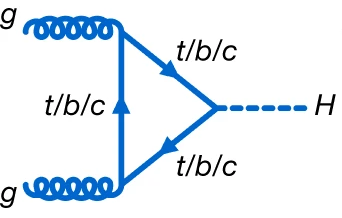
\includegraphics[width=0.3\linewidth]{images/ggF.png}  &
        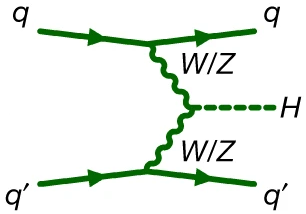
\includegraphics[width=0.3\linewidth]{images/VBF.png}  &
        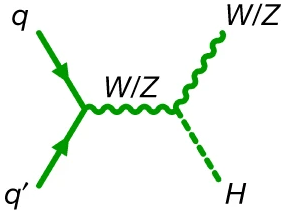
\includegraphics[width=0.3\linewidth]{images/VH.png}   \\
        (a) $ggF$ & (b) $VBF$ & (c) $VH$ \\
    \end{tabular}
    \vspace{0.5em} % Espacio entre filas
    % Segunda fila: 2 imágenes centradas bajo las 3 primeras
    \makebox[\textwidth][c]{%
        \begin{tabular}{cc}
            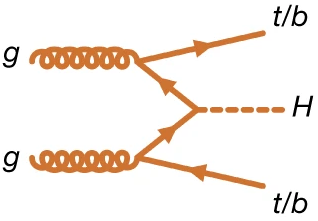
\includegraphics[width=0.3\linewidth]{images/ttH.png} &
            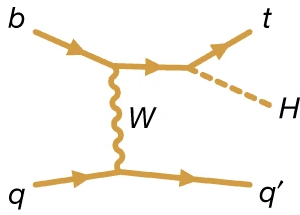
\includegraphics[width=0.3\linewidth]{images/tH.png} \\
            (d) $t\bar{t}(b\bar{b})H$ & (e) $tH$ \\
        \end{tabular}%
    }
    \caption{
    Examples of leading order Feynman diagrams for Higgs-boson production modes at the LHC~\cite{Nature_ATLAS}.}
    \label{fig:higgs_production}
\end{figure}

\begin{figure}[htbp]
    \centering
    
    \begin{subfigure}[b]{0.46\textwidth}
        \centering
        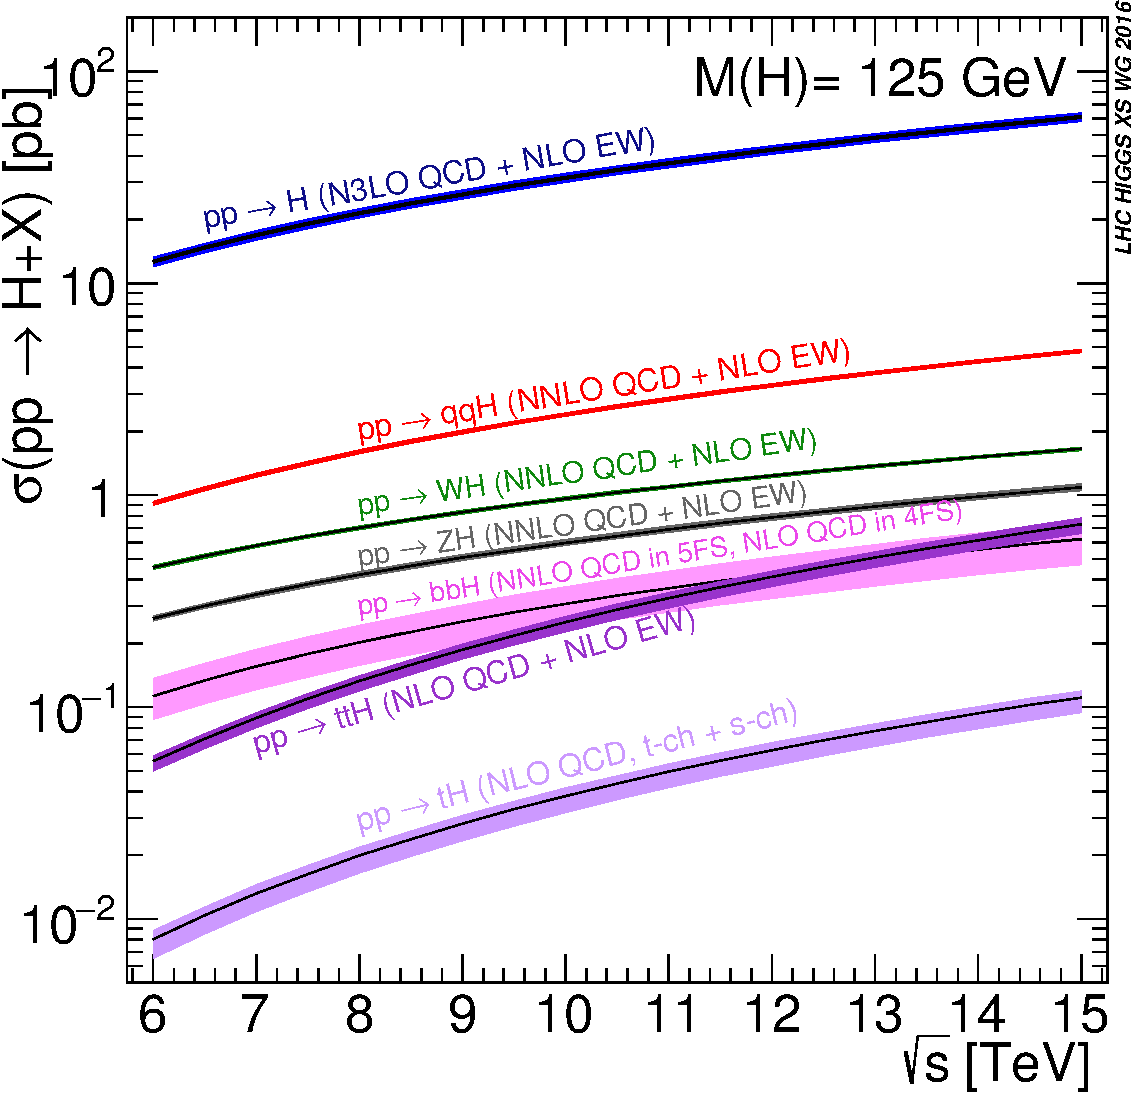
\includegraphics[width=\linewidth]{images/higgs_prod.pdf}
        \caption{}
        \label{fig:higgs_comb:prod}
    \end{subfigure}
    \hfill
    \begin{subfigure}[b]{0.46\textwidth}
        \centering
        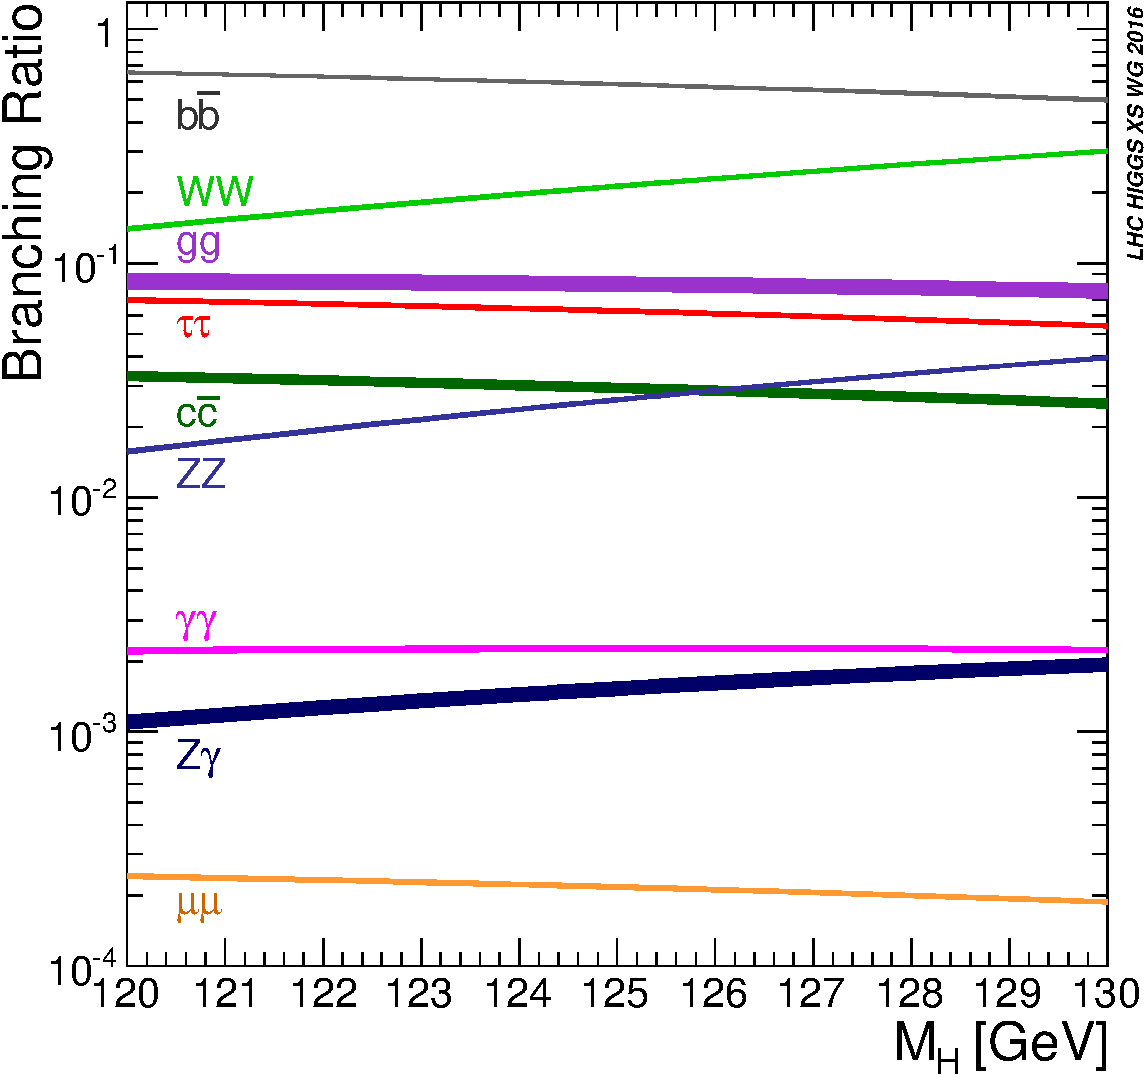
\includegraphics[width=\linewidth]{images/higgs_dec.pdf}
        \caption{}
        \label{fig:higgs_comb:dec}
    \end{subfigure}

    \caption{(a) Cross-sections measured for Higgs boson production as a function of the center of mass energy in proton-proton collisions. (b) Branching ratios for the different Higgs boson decay modes as a function of the Higgs boson mass~\cite{Nature_ATLAS}.}    \label{fig:higgs_comb}
\end{figure}



The dominant production mode is gluon-gluon fusion (ggF), where two gluons from the colliding protons interact via a heavy quark loop, primarily involving the top quark, to produce a Higgs boson. This process accounts for about 90\% of the total Higgs boson production cross-section at the LHC energies, due to the high gluon density within the proton.

Another important channel is vector boson fusion (VBF), responsible approximately $7\%$ of the total production cross-section. The Higgs boson is produced via a $t$-channel exchange of two weak bosons radiated from the incoming quarks. This mechanism is characterized by the presence of two high-momentum hard jets emitted at small angles from the colliding protons, while the Higgs boson is tipically produced between them in the central region, offering a clean and efficient experimental signature. 

Associated production with a vector boson ($VH$), where the Higgs boson is produced alongside a $W$ or $Z$ boson, is particularly useful in final states with leptons, providing strong handles for background discrimination in a hadronic environment. It provides around the $4\%$ of the Higgs boson production cross-section.

Finally, the associated production with a pair of top quarks ($t\bar{t}H$) provides a direct probe of the Yukawa coupling between the Higgs boson and the top quark, the strongest coupling in the SM. Although its production cross-section is significantly lower than other channels, around $1\%$ of the total, it plays a strategic role in testing the interaction responsible for the top-quark mass generation, which will be discussed in the following.
The rarest considered production mode is the associated production with a single top quark, accouting for approximately $0.2\%$. This process could also contribute to the direct determination of the top-quark Yukawa coupling. However, its production cross-section is significantly smaller than \( t\bar{t}H \) production. Furthermore, additional LO diagrams for $tH$ production involve the $WH$ coupling, which already blurs the measurement.

Additionally, there are other production modes that remain experimentally challenging, such as Higgs boson production in association with bottom quark pairs, \( b\bar{b}H \). While this mode has a production cross-section comparable to that of \( t\bar{t}H \), it suffers from a much less clean experimental signature due to the large background contribution from multijet production.

%xxxxxxxxxxxxxxxxxxxxxxxxxxxxxxxxxxxxxxxxxxxxxxxxxxxxxx
\subsubsection*{Higgs boson decay modes}
\label{sec:higgs_decay}
%xxxxxxxxxxxxxxxxxxxxxxxxxxxxxxxxxxxxxxxxxxxxxxxxxxxxxx

The SM Higgs boson, with a lifetime of approximately \(10^{-22}\) seconds, decays into a wide range of experimentally accessible final states that enable its observation, as its extremely short existence precludes direct detection.

As mentioned in Section~\ref{subsec:higgs_mech}, the coupling of the Higgs boson to fermions is proportional to the fermion mass, while for gauge bosons the coupling is proportional to \(m_Z^2\) and \(m_W^2\) in the \(HZZ\) and \(HWW\) vertices, respectively. Consequently, the Higgs boson decays preferentially into the heaviest particles kinematically allowed.

Figure~\ref{fig:higgs_comb:dec} shows the predicted branching ratios for the decay of the SM Higgs boson as a function of its mass. Representative Feynman diagrams for the dominant decay modes are shown in Figure~\ref{fig:h_decays}.
\begin{figure}[htbp]
    \centering
    
    % Primera fila
    \begin{subfigure}[b]{0.3\linewidth}
        \centering
        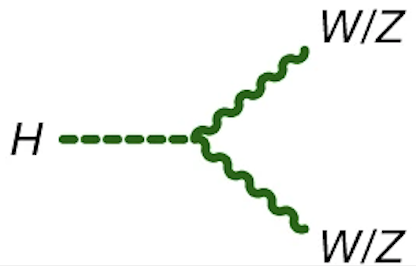
\includegraphics[width=\linewidth]{images/HVV.png}
        \caption{}
        \label{fig:h_decays:VV}
    \end{subfigure}
    \hfill
    \begin{subfigure}[b]{0.3\linewidth}
        \centering
        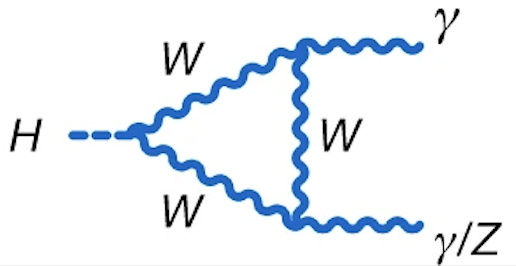
\includegraphics[width=\linewidth]{images/Hgg.png}
        \caption{}
        \label{fig:h_decays:gg}
    \end{subfigure}
    \hfill
    \begin{subfigure}[b]{0.3\linewidth}
        \centering
        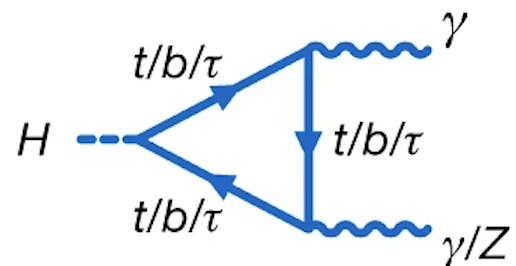
\includegraphics[width=\linewidth]{images/Hgg_loop.png}
        \caption{}
        \label{fig:h_decays:Zg}
    \end{subfigure}
    
    \vspace{0.7em} % Espacio entre filas
    
    % Segunda fila
    \begin{subfigure}[b]{0.3\linewidth}
        \centering
        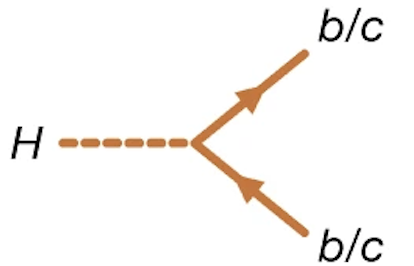
\includegraphics[width=\linewidth]{images/Hbb.png}
        \caption{}
        \label{fig:h_decays:bb}
    \end{subfigure}
    \hspace{0.1\linewidth}
    \begin{subfigure}[b]{0.3\linewidth}
        \centering
        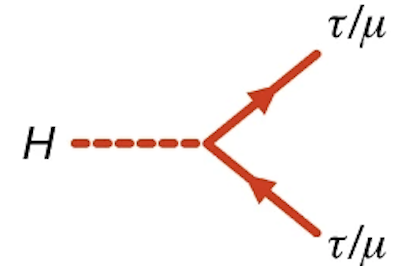
\includegraphics[width=\linewidth]{images/Htt.png}
        \caption{}
        \label{fig:h_decays:tautau}
    \end{subfigure}
    
    \caption{Representative LO Feynman diagrams for the main decay modes of a Higgs boson of 125 GeV to (a) a pair of vector bosons, (b),(c) a pair of photons or a $Z$ boson and a photon, (d) a pair of quarks, and (e) a pair of charged leptons~\cite{Nature_ATLAS}.}
    \label{fig:h_decays}
\end{figure}

The Higgs boson predominantly decays into a pair of bottom quarks, \( H \rightarrow b\bar{b} \), with a branching ratio ($\mathcal{B}$) of approximately \( \mathcal{B}(H \rightarrow b\bar{b}) \approx 0.581 \). However, the measurement of this decay mode at the LHC is challenging due to the overwhelming background from multijet production. Despite this, its large branching ratio motivates dedicated studies, especially in channels involving the associated production of a Higgs boson with a vector boson, which enhances the analysis sensitivity.

Decays into pairs of gauge bosons are suppressed, since at least one of the two bosons must be produced off-shell due to the mass of the Higgs boson. The corresponding branching ratios are approximately \( \mathcal{B}(H \rightarrow WW^*) \approx 0.22 \) and \( \mathcal{B}(H \rightarrow ZZ^*) \approx 0.03 \). Among these, the \( H \rightarrow ZZ^* \) decay mode stands out due to its clean experimental signature and high resolution, as the $Z$ bosons can decay fully leptonically into pairs of electrons or muons that are efficiently reconstructed and identified in the detector. 
In contrast, the \( H \rightarrow WW^* \) channel is experimentally more challenging: while the $W$ bosons may decay hadronically, producing jets that are difficult to distinguish from the overwhelming QCD background, their leptonic decays unavoidably involve neutrinos that escape detection, leading to missing energy and degrading the mass resolution. This makes the reconstruction of the Higgs boson in this channel substantially more difficult compared to the four-lepton final state of \( H \rightarrow ZZ^* \).

The Higgs boson can also decay into a pair of photons, \( H \rightarrow \gamma\gamma \), via a one-loop radiative process involving virtual top quarks, as can be seen in Figure~\ref{fig:h_decays:Zg}, or $W$ boson loops, as shown in Figure~\ref{fig:h_decays:gg}. Although this decay has one of the lowest branching ratios, with \( \mathcal{B}(H \rightarrow \gamma\gamma) \approx 0.227\% \), it plays a key role in Higgs boson studies at the LHC due to its excellent signal-to-background ratio. This leads to a very clean experimental signature with high resolution, especially when compared to the background from prompt photon pair production.

The decay into a pair of $\tau$-leptons is also possible for the Higgs boson, with a branching ratio of approximately \( \mathcal{B}(H \rightarrow b\bar{b}) \approx 6\% \). This decay mode plays a central role in this thesis. From the experimental point of view, the $H \rightarrow \tau\tau$ decay presents several challenges. First, the presence of neutrinos in $\tau$-lepton decays prevents a full reconstruction of the di-$\tau$ final state, complicating the determination of the Higgs boson mass. To overcome this limitation, advanced reconstruction techniques must be employed to estimate the mass of the di-$\tau$ system.

In addition, the $H \rightarrow \tau\tau$ decay is affected by a significant irreducible background from $Z \rightarrow \tau\tau$ events, whose production cross-section is several orders of magnitude larger than that of the Higgs boson. Despite these difficulties, this decay channel offers an unique opportunity to probe the Yukawa interaction between the Higgs boson and the $\tau$-lepton, providing the most precise measurement of a fermionic coupling to date due to its relatively large branching ratio. Furthermore, it allows for the study of the $CP$ properties of the Higgs boson, both in its production mechanisms and decay, and offers good sensitivity to the VBF production mode.

In the context of the Yukawa sector, the SM also predicts Higgs boson decays to fermions of the first and second generation. The decay into muons, \( H \rightarrow \mu\mu \), although having a very small branching ratio of about 0.02\%, presents a clean experimental signature with two well-reconstructed muons in the final state. However, its measurement is significantly affected by the large background from the Drell--Yan production ($Z/\gamma* \to \mu \mu$). On the other hand, the \( H \rightarrow c\bar{c} \) decay has a larger branching ratio of approximately 2.9\%, but its measurement at the LHC is challenged by the large multijet background. In addition, the identification of charm quarks remains a difficult task in the environment of a hadron collider. Decays of the Higgs boson to lighter fermions have exceedingly small branching fractions, rendering their direct observation unfeasible with current experimental sensitivity~\cite{https://doi.org/10.23731/cyrm-2017-002}.

%xxxxxxxxxxxxxxxxxxxxxxxxxxxxxxxxxxxxxxxxxxxxxxxxxxxxxx
\subsection{The \ttH process: a gateway to the Yukawa sector}
\label{sec:ttH}
%xxxxxxxxxxxxxxxxxxxxxxxxxxxxxxxxxxxxxxxxxxxxxxxxxxxxxx
As already highlighted in previous sections, the top-quark Yukawa coupling, $y_t$, is the strongest among all SM fermions, owing to the large mass of the top quark. This makes $y_t$ particularly sensitive to possible BSM contributions and an essential parameter to explore the nature of electroweak symmetry breaking~\cite{Englert:2014uua,Dobrescu:1997nm,Chivukula:1998wd,Delepine:1995qs}. Moreover, direct access to $y_t$ is crucial for probing the $CP$ structure of the Higgs sector~\cite{Bernreuther:2002uj,Brod:2013cka}, and plays an indirect role in constraining the Higgs field self-coupling~\cite{Buttazzo:2013uya,Degrassi:2016wml}.

While a direct measurement via the $H\to t\bar{t}$ decay is not accessible due to kinematic suppression due to the large mass of the top quarks, $t\bar{t}H$ offers an unique and direct probe of $y_t$. Contrary to ggF, where the coupling appears in a quantum loop that may receive BSM contributions, the \ttH process provides tree-level sensitivity to $y_t$, being the production cross-section proportional to the coupling. This complementarity is particularly useful when comparing indirect constraints from loop-induced processes to direct measurements~\cite{Ng:1983jm,Kunszt:1984ri,Beenakker:2001rj}.

The \ttH production mode was first observed in 2018 by the ATLAS and CMS collaborations~\cite{ATLAS:2018mme,CMS:2018uxb}, following the combination of multiple analyses targeting different Higgs boson decay channels. Among these channels, the $H\to b \bar{b}$ and $H\to \gamma \gamma$ analyses provided the first hints due to their high branching ratio or clean experimental signature, respectively. However, both channels come with significant limitations: the former suffers from large backgrounds with $b$-jets and sizeable modeling uncertainties, while the latter is constrained by its low branching fraction.

In addition, the so-called ``multilepton analysis'' (\ttH(ML)) constitutes another powerful probe of $t\bar{t}H$ production, targeting final states with multiple light leptons (electrons and muons) and hadronically decaying $\tau$-leptons. These signatures arise predominantly from Higgs decays into $WW^*$ or $ZZ^*$, as well as from leptonic decays of $\tau$-leptons, leading to complex final states with high lepton multiplicity. The multilepton channel benefits from relatively clean experimental signatures and good background suppression, although it is statistically limited due to the small branching fractions of these decays. Within ATLAS, the $t\bar{t}H$(ML) analysis has become one of the most sensitive channels in the overall $t\bar{t}H$ combination.

Among the Higgs boson decay modes, the $H\to\tau\tau$ channel offers an alternative strategy that strikes a balance between statistical power and experimental cleanliness. Its branching ratio is significantly larger than that of $H\to \gamma \gamma$, and although $\tau$-leptons are more challenging to reconstruct than electrons or muons, they lead to final states with relatively low backgrounds and good experimental sensitivity.

The analysis of $t\bar{t}H$ production with $H\to\tau\tau$ decays is often grouped with other multilepton channels ($H\to WW^*, ZZ^*$) due to similarities in event topology. However, the main analysis presented in this thesis focuses on the specific case where both $\tau$-leptons decay hadronically. This channel is not included within the leptonic or semileptonic categories of the $t\bar{t}H$(ML) analysis. Instead, it is treated as part of the dedicated $H\to\tau\tau$ analysis. In Chapter~\ref{chap:htautau}, the distinctive experimental signature and the potential of this process will be exploited.
%xxxxxxxxxxxxxxxxxxxxxxxxxxxxxxxxxxxxxxxxxxxxxxxxxxxxxx
\subsection{Measurements of production cross-section and branching ratios: the STXS framework}
\label{sec:stxs_yukawa}
%xxxxxxxxxxxxxxxxxxxxxxxxxxxxxxxxxxxxxxxxxxxxxxxxxxxxxx
Measurements targeting a Higgs boson signal commonly focus on determining a signal strength modifier, denoted as $\mu$. This parameter is defined as the ratio of the measured production cross-section times the branching ratio to the corresponding SM prediction:
\begin{equation}
\label{signal_strength}
    \mu = \frac{\sigma \times \mathcal{B}}{\sigma_{\mathrm{SM}} \times \mathcal{B}_{\mathrm{SM}}},
\end{equation}
where $\sigma$ denotes the production cross-section and \mathcal{B} the decay branching ratio.

Such measurements aim to maximize sensitivity to the Higgs boson signal by comparing observed event yields in data to the expected yields from the SM for each of the main Higgs boson production modes.

During the Run-2 period of the LHC, all the main Higgs boson production and decay modes have been observed with varying degrees of significance. The latest combined results from the ATLAS experiment for production cross-section and decay branching ratio measurements show a remarkable agreement with SM expectations, as illustrated in Figure~\ref{fig:higgs_mu}, resulting in a measured inclusive signal strength of $\mu = 1.05 \pm 0.06$~\cite{Nature_ATLAS}. Similar value was obtained by the CMS collaboration~\cite{CMS:2022dwd}. Evidence for rare decay modes, such as $H \to Z\gamma$ and $H \to \mu\mu$, has also been reported~\cite{Aad_2024,muon2021}.

\begin{figure}[htbp]
    \centering
    \subfloat[(a)]{
        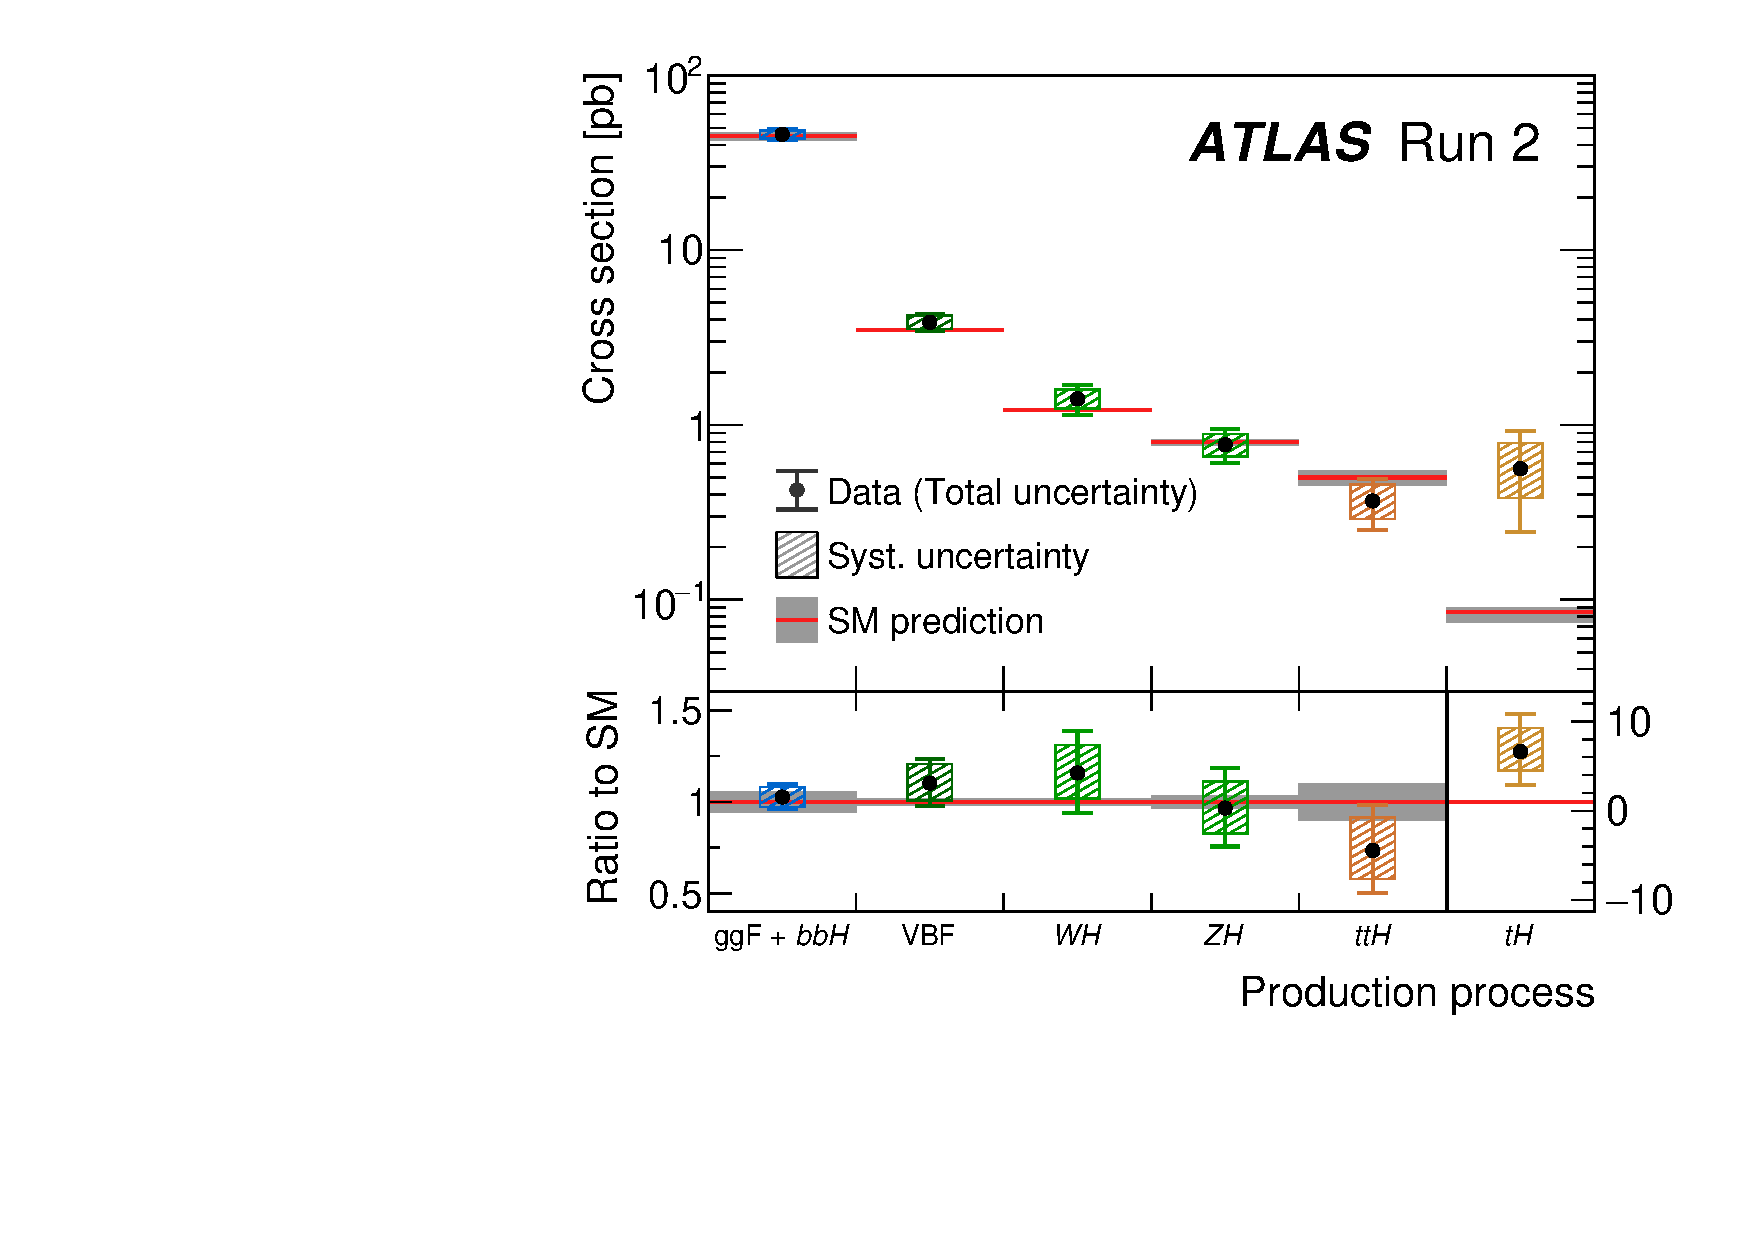
\includegraphics[width=0.46\textwidth]{atlas_combined_xsect.pdf}
    }
    \hfill
    \subfloat[(b)]{
        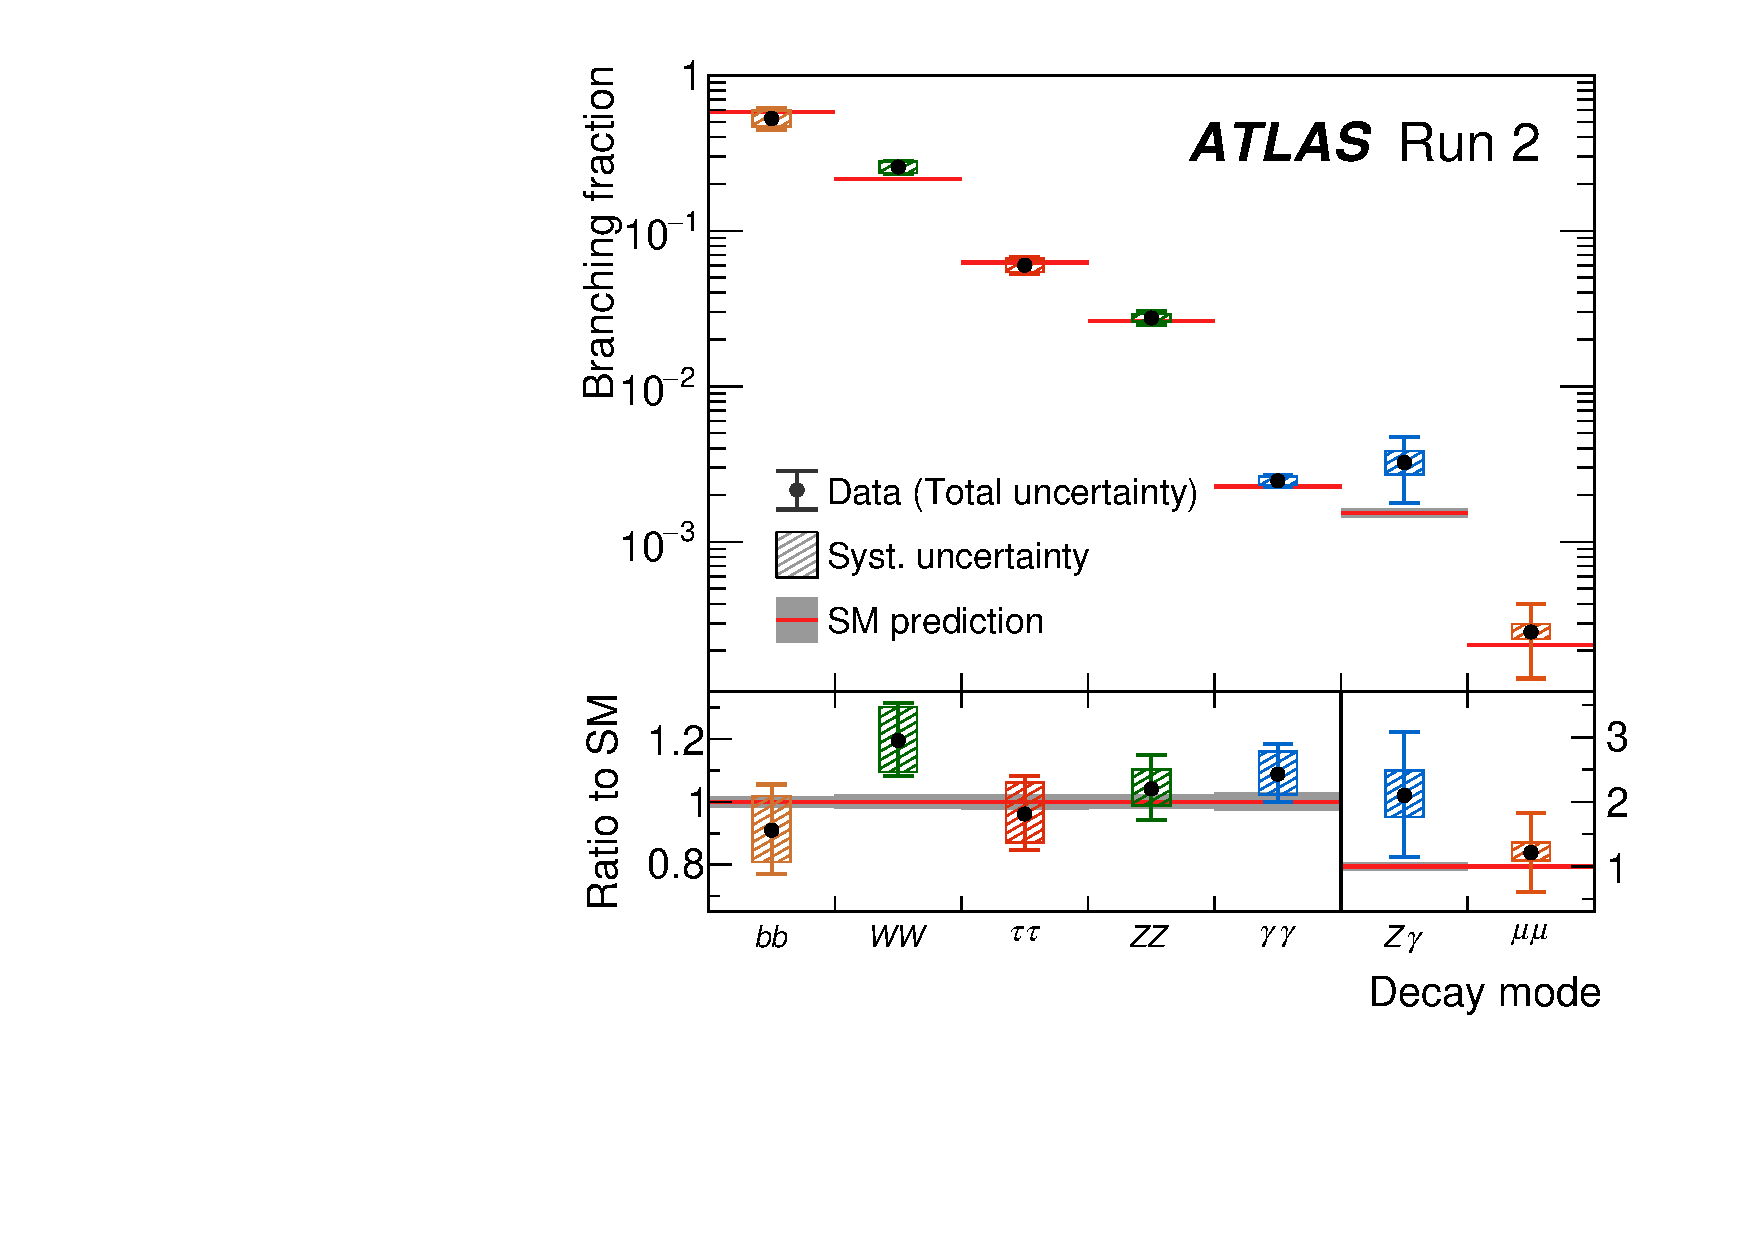
\includegraphics[width=0.46\textwidth]{atlas_combined_br.pdf}
    }
    \caption{(a) Summary of the Higgs boson production cross-sections assuming SM values for the Higgs boson branching ratios. 
    (b) Measurements of the Higgs boson decay branching ratios assuming SM predictions for the production cross-sections. 
    All results are obtained using ATLAS Run-2 data, combining different analyses, and are consistent with the SM predictions within uncertainties~\cite{Nature_ATLAS}.}
    \label{fig:higgs_mu}
\end{figure}


Despite their overall success, these inclusive measurements exhibit limited sensitivity to BSM effects that could manifest in specific phase space regions where few signal events are expected. Furthermore, these inclusive analyses depend heavily on theoretical predictions, as the uncertainty in the global signal strength $\mu$ is directly influenced by the uncertainties in the SM production cross-section and branching ratio calculations that are assumed. Additionally, analysis strategies and event selection criteria typically assume SM kinematics for the expected signal, which may reduce sensitivity to BSM scenarios.

An alternative approach to reduce the dependence on SM theoretical extrapolations is the measurement of fiducial production cross-sections. In these analyses, a fiducial phase space is defined at particle level\footnote{The particle level indicates the level in which all the physical objects are defined using stable particles in their final states, after parton shower and hadronisation, but without any interaction with the detector.}, designed to closely resemble the reconstructed event selections to minimize the extrapolation from the measured phase space. Detector effects are corrected using simulations, allowing a direct comparison of the measured fiducial production cross-section with theoretical predictions. However, the requirement of similar selections at particle and detector levels often necessitates simplified event selections, which might not be optimal for signal-to-background discrimination. The use of multivariate techniques is typically limited in fiducial measurements due to the complexity of mapping reconstructed variables to particle-level definitions.

Fiducial production cross-section measurements can be further extended to differential production cross-section measurements, where the production rates are measured as functions of relevant kinematic observables. These measurements provide richer information on the Higgs boson production dynamics and possible deviations from SM predictions.

To find a balance between inclusive and fiducial differential measurements, the Simplified Template production cross-section (STXS) framework was developed~\cite{badger2016leshouches2015physics}. The STXS framework partitions the Higgs boson production phase space into multiple exclusive regions or bins, each defined by kinematic criteria involving the Higgs boson and associated objects in the final states such as jets or vector bosons. This binning scheme is optimized to enhance sensitivity to possible BSM effects while keeping a reasonable independence and control over theoretical uncertainties.

STXS measurements offer differential information about Higgs boson production, allowing the use of complex multivariate analysis techniques in event selections. This is particularly advantageous for decay channels with challenging final-state reconstruction, such as $H \to \tau\tau$ or $H \to b\bar{b}$, where detector resolution and background contamination are more significant compared to cleaner channels like $H \to \gamma\gamma$ or $H \to ZZ^*$.

The STXS framework also facilitates the combination of results from analyses targeting different Higgs boson decay modes, maximizing the overall experimental sensitivity. The current binning scheme, referred to as Stage 1.2~\cite{STXS11} and shown in Figure~\ref{fig:STXSbins}, refines the granularity introduced in earlier stages (so-called Stage 1.1~\cite{STXS11}) to better exploit the available data. 

\begin{figure}[htbp]
    \centering
    \begin{overpic}[width=0.6\linewidth]{images/STXSbins_ggF}
        \put(95,5){\small (a)}
    \end{overpic}\\[0.3cm]
    \begin{overpic}[width=0.6\linewidth]{images/STXSbins_VBF_VqqH}
        \put(98,5){\small (b)}
    \end{overpic}\\[0.3cm]
    \begin{overpic}[width=0.6\linewidth]{images/STXSbins_VlepH}
        \put(98,5){\small (c)}
    \end{overpic}\\[0.3cm]
    \begin{overpic}[width=0.25\linewidth]{images/STXSbins_ttH}
        \put(95,5){\small (d)}
    \end{overpic}
    \caption{STXS stage 1.2 bin definition for (a) ggF production, 
    (b) VBF production and associated production with a hadronically decaying vector boson, 
    (c) associated production with a leptonically-decaying vector boson and 
    (d) \ttH. The representation of $tH$ is omitted as it only consists of one bin~\cite{STXS11}.}
    \label{fig:STXSbins}
\end{figure}

Higgs boson production modes are classified into categories within the STXS scheme, based on the production mechanism and associated particles:

\begin{itemize}
    \item \textbf{Gluon-gluon fusion ($gg \to H$)}: including the dominant ggF process and gluon-induced associated production with a $Z$ boson decaying hadronically, $gg \to ZH \to q\bar{q}H$. Production of $b\bar{b}H$ is also included here.
    \item \textbf{EWK $qq'\to qq'H$}: it includes the Higgs boson production via VBF and the quark-initiated associated production of a Higgs boson with a vector boson where the vector boson decays hadronically ($qq'\to VH \to qq'H$).
    \item \textbf{Vector boson associated production ($VH \to (\ell \ell, \ell\nu)H$)}: Higgs boson produced in association with a $W$ or $Z$ boson decaying leptonically.
    \item \textbf{Top-associated production ($t\bar{t}H$ and $tH$)}: Higgs boson produced with a top quark pair or single top quark.
\end{itemize}

Within each category, the STXS bins are further subdivided based on key variables such as the transverse momentum of the Higgs boson ($p^H_\{\text{T}}$) or vector boson ($p^V_{\text{T}}$), the number of jets, and the dijet invariant mass. The binning scheme is flexible and can be adapted to the experimental sensitivity: bins with insufficient data can be merged, and finer bins can be introduced as more data becomes available.

The latest combination of ATLAS Run-2 data using the STXS framework has produced measurements of the Higgs boson production cross-section in 36 exclusive kinematic regions~\cite{Nature_ATLAS}. The results are consistent with SM predictions, providing stringent constraints on BSM scenarios. Figure~\ref{fig:atlas-stxs-results} summarizes these measurements.

\begin{figure}[htbp]
    \centering
    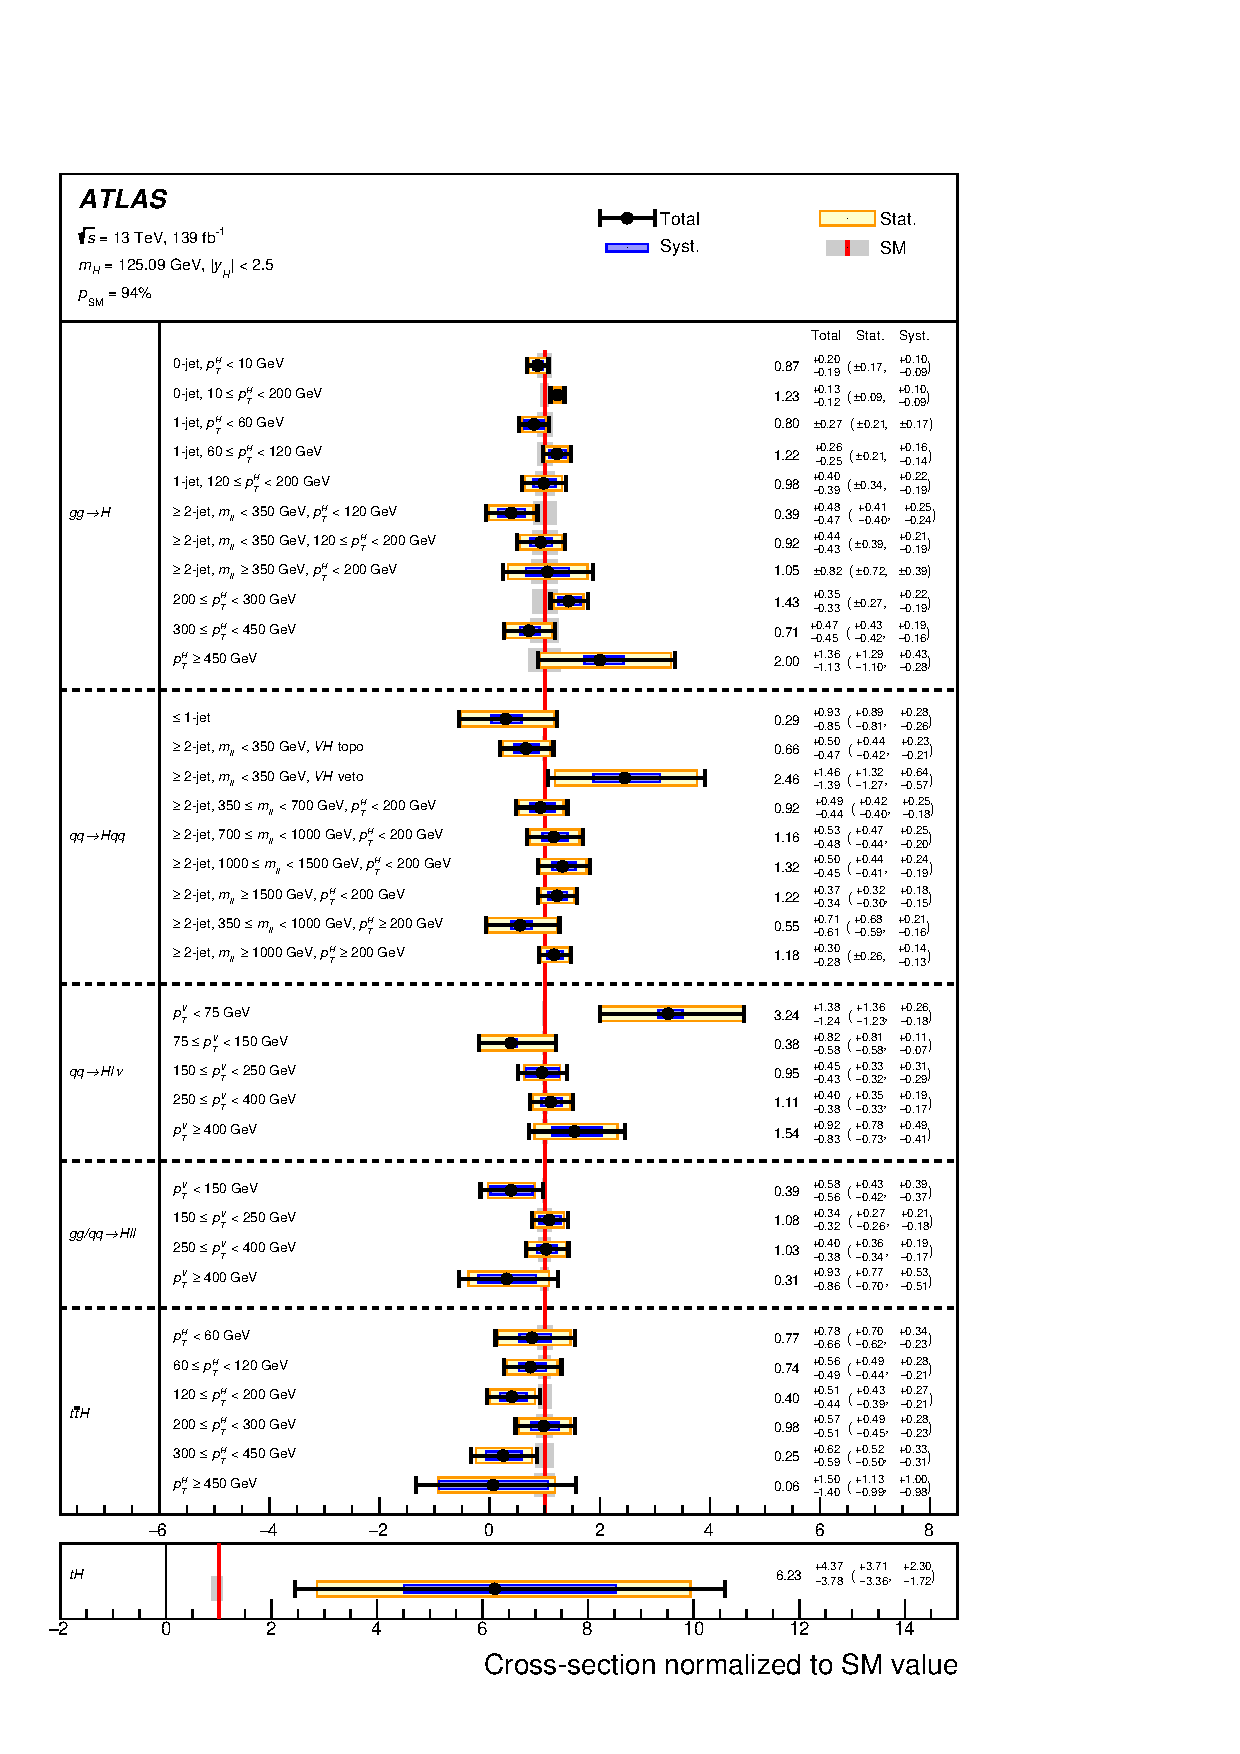
\includegraphics[width=0.75\textwidth]{atlas_stxs_results.pdf}
    \caption{Measurement of the Higgs boson production cross-section normalized to the SM predictions in 36 exclusive STXS regions using ATLAS Run-2 data. All these results are obtained assuming SM branching ratios for the Higgs boson decays. The error bars represent the total uncertainty in the measurement (in black), the statistical uncertainty (in yellow) and the systematic uncertainty (in blue)~\cite{Nature_ATLAS}.}
    \label{fig:atlas-stxs-results}
\end{figure}

This thesis contributes to extending the STXS measurements in the $H \to \tau \tau$ decay channel, with particular emphasis on the $t\bar{t}H$ production mode. The analysis strategy and detailed results are presented in Chapter~\ref{chap:htautau}. Note that the results shown in Figure~\ref{fig:atlas-stxs-results} do not yet include the $H \to \tau \tau$ channel measurements presented in this document.


%-------------------------------------------------------------------------------

%-------------------------------------------------------------------------------
\chapter{The LHC and the ATLAS Experiment}
\label{chap:ATLAS}
This chapter presents the experimental setup that has made possible the studies discussed throughout this thesis. It introduces the Large Hadron Collider (\acrshort{lhc}), a proton--proton collider located at the research complex of the Conseil Européen pour la Recherche Nucléaire (\acrshort{cern}). Subsequently, a description of the ATLAS (A Toroidal LHC ApparatuS) detector is provided, as it is the experiment from which the data used in this analysis have been collected.

%++++++++++++++++++++++++++++++++++++++++++++++
\section{The Large Hadron Collider}
\label{sec:LHC}
%++++++++++++++++++++++++++++++++++++++++++++++

The Large Hadron Collider (\acrshort{lhc}) is the world's largest and most powerful particle accelerator, situated at the \acrshort{cern} laboratory near Geneva, on the border between Switzerland and France. Founded in 1954, CERN is a European intergovernmental organization with the primary mission of advancing fundamental research in high-energy physics. It has become a global hub for scientific collaboration, involving over 20 member states and thousands of scientists and engineers from across the world.

The \acrshort{lhc} is the flagship project of \acrshort{cern}'s accelerator complex, and represents one of the most ambitious scientific endeavours in history. Its primary goals include performing precision measurements of \acrshort{sm} processes in order to be sensitive to any possible deviation, and searching for signs of new physics phenomena beyond the current theoretical framework, such as supersymmetry, extra dimensions, or dark matter candidates, as discussed in Section~\ref{sec:BSM}. The LHC's predecessor in the energy frontier was the Tevatron collider at Fermilab (USA), which operated at a centre-of-mass energy of 1.96~TeV. With its design energy of up to 14~TeV, the LHC has dramatically extended the discovery potential in the high-energy frontier, culminating in landmark achievements such as the discovery of the Higgs boson in 2012~\cite{ATLAS:2012yve,CMS:2012qbp}.

%xxxxxxxxxxxxxxxxxxxxxxxxxxxxxxxxxxxxxxxxxxxxxxxxxxxxxx
\subsection*{Overview and layout of the LHC}
%xxxxxxxxxxxxxxxxxxxxxxxxxxxxxxxxxxxxxxxxxxxxxxxxxxxxxx

The \acrshort{lhc} is a nearly circular accelerator with a circumference of 27~km, located about 100~m underground~\cite{Lyndon:Evans_2008}. It consists of two counter-rotating beam pipes, each containing a beam of protons (or heavy ions in some cases), which are accelerated to ultra-relativistic energies and made to collide at specific interaction points. These collision points are surrounded by four main detectors: \acrshort{atlas}, \acrshort{cms}, \acrshort{alice}, and \acrshort{lhcb}, each optimized for different types of physics analyses. While \acrshort{atlas}~\cite{ATLAS:exp} and \acrshort{cms}~\cite{CMS:exp} are general-purpose detectors designed to explore a broad range of physics topics, \acrshort{alice}~\cite{ALICE:exp} focuses on the beforehand mentioned heavy-ion collisions to study the quark–gluon plasma, and \acrshort{lhcb}~\cite{LHCb:exp} specializes in flavour physics and CP violation in the decays of heavy-flavour hadrons.

Protons are injected into the \acrshort{lhc} via a complex chain of smaller accelerators. Firstly, hydrogen atoms are ionized and resulting protons are accelerated up to 50~MeV by the linear accelerator, the LINAC2. They are then injected in the Proton Synchrotron Booster (PSB), which is followed by the Proton Synchrotron (PS) and the Super Proton Synchrotron (SPS), ending with the beams of protons reaching energies of 1.4~GeV, 26~GeV and 450~GeV, respectively. All these stages are represented in Figure~\ref{LHC:chain}. The PS and SPS pack protons to the LHC ring in bunches, which in nominal conditions are separated by 25 ns and a total of 2808 bunches can be finally delivered. Each of these bunches, containing around $10^{11}$ protons, are kept circulating inside the \acrshort{lhc} using superconducting magnets (mainly dipoles and quadrupoles) cooled to 1.9~K with liquid helium. Bending and focusing of the proton beams is needed since, as mentioned, the \acrshort{lhc} ring is not really circular, 
but composed of eight arcs and eight straight sections between them, 520 meters long each. This straight sections connects to the surface installations by lifts, where the main experiments mentioned above are located.

\begin{figure}[htbp]
    \centering
    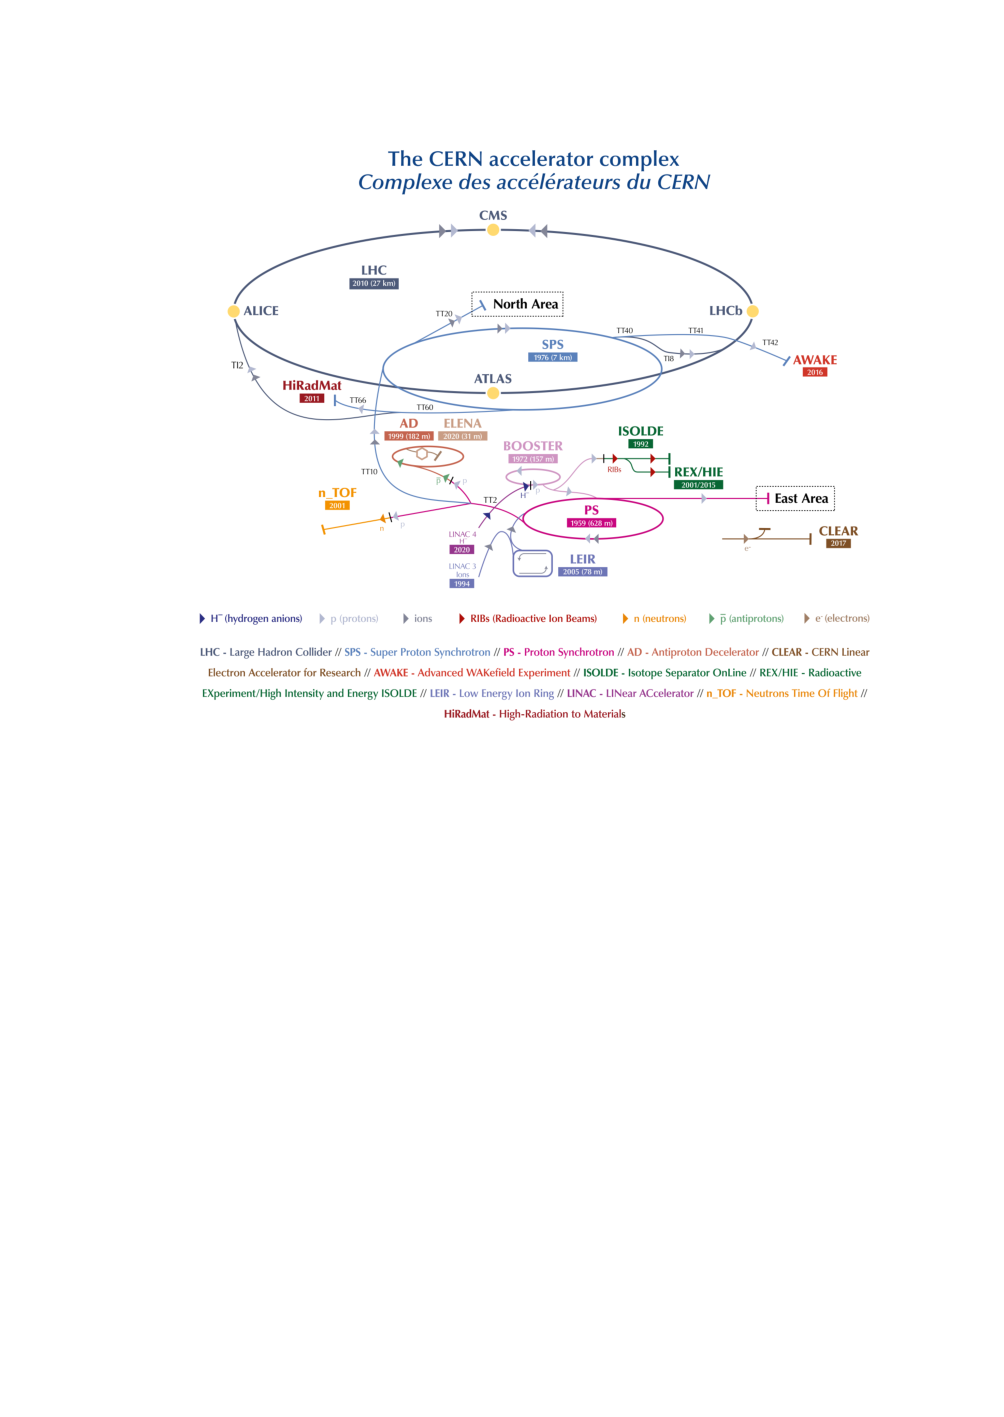
\includegraphics[width=1\linewidth]{images/CCC-v2022}\\
    \caption{Schematic overview of the CERN accelerator complex: the Large Hadron Collider, its injection chain and the four main experiments that record the collisions~\cite{Lopienska:2800984}}
    \label{LHC:chain}
\end{figure}


%xxxxxxxxxxxxxxxxxxxxxxxxxxxxxxxxxxxxxxxxxxxxxxxxxxxxxx
\subsection*{Beam conditions and luminosity}
%xxxxxxxxxxxxxxxxxxxxxxxxxxxxxxxxxxxxxxxxxxxxxxxxxxxxxx

Besides the energy that LHC can deliver to the colliding protons, another important performance characteristic of the accelerator is the number of events it is capable of producing. If one considers the instantaneous luminosity as a measure of the particle flux, then in a scattering process such as proton--proton collisions, the number of collisions can be expressed as:

\begin{equation}
  N_\text{{events}} = \sigma_{\text{event}} \int L\text{d}t = \sigma_{\text{event}}\mathcal{L},
\end{equation}
which is proportional to the cross-section representing the underlying physics of the process of interest, $\sigma_{\text{event}}$, such as Higgs boson production. The time integral over the instantaneous luminosity is referred to as the integrated luminosity, $\mathcal{L}$. The instantaneous luminosity depends on the properties of the beams and can be expressed as follows~\cite{Aad_2023}:
\begin{equation}
    L = f_{\text{rev}}\frac{N_1 N_2 N_b}{4\pi \sigma_x \sigma_y},
\end{equation}
where $N_b$ is the number of bunches per beam, $N_1$ and $N_2$ are the number of protons per bunch and $f_{\text{rev}}$ is the revolution frequency. In practice not all bunches are filled with electrons, and moreover these proton packs have extensions in both two directions perpendicular to the beam propagation direction assuming an effective gaussian shape with area $4\pi\sigma_{x}\sigma{y}$, being $\sigma_{x}$ and $\sigma_{y}$ the horizontal and vertical gaussian widths respectively.  

The integrated luminosity is typically expressed in units of inverse femtobarns (fb$^{-1}$), where $1~\text{fb}^{-1} = 10^{39}~\text{cm}^{-2}$. Figure~\ref{figure:Run3lumi}(a) shows the integrated luminosity delivered to ATLAS for each year of data taking from 2011 to 2025. Figure~\ref{figure:Run3lumi}(b) displays a comparison between the cumulative luminosity delivered and recorded by the ATLAS detector during Run~2, the data-taking period from 2015 to 2018, which constitutes the main dataset analysed in this thesis, along with the early years of Run~3.

\acrshort{atlas} collected approximately 147~fb$^{-1}$ of proton--proton collision data at a center-of-mass energy of 13~TeV during Run~2. However, not all delivered data are suitable for physics analysis. The dataset certified for physics-quality analyses, i.e.\ the one included in the Good Run List (GRL)~\cite{Aad_2020}, is slightly smaller due to quality and detector performance criteria. Specifically, ATLAS recorded a total of $140 \pm 1.2$~fb$^{-1}$ of high-quality data during Run~2, and approximately 166~fb$^{-1}$ during the years 2022--2024 of Run~3.

\begin{figure}[htbp]
\centering
\begin{tabular}{cc}
    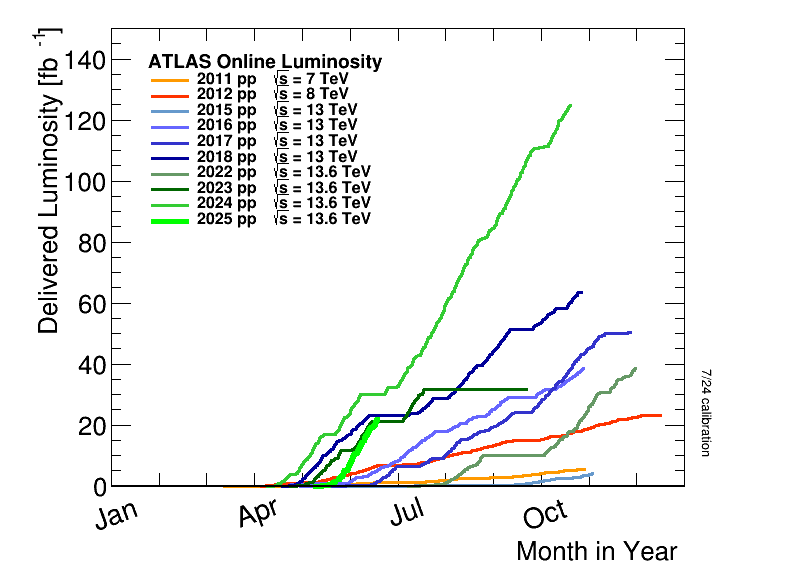
\includegraphics[width=0.5\linewidth]{images/intlumivsyear.png} &
    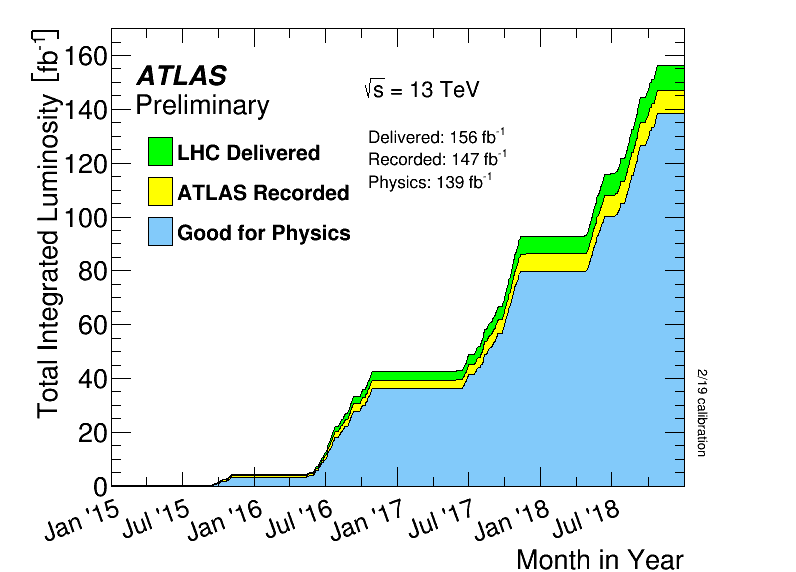
\includegraphics[width=0.5\linewidth]{images/intlumivstimeRun2DQall.png} \\
    (a) & (b)  \\
\end{tabular}
\caption{(a) Cumulative pp collision luminosity delivered to the ATLAS detector versus month
of the year, separately for years between 2011 and 2024~\cite{atlas:Run3lumi} and (b) cumulative luminosity versus
time delivered by the LHC (green), recorded by ATLAS (yellow) and used for physics (blue)
during stable beams for pp collisions at 13 TeV centre-of-mass energy in years 2015-2018~\cite{atlas:Run2lumi}}
\label{figure:Run3lumi}
\end{figure}

%xxxxxxxxxxxxxxxxxxxxxxxxxxxxxxxxxxxxxxxxxxxxxxxxxxxxxx
\subsection*{Pile-up and its challenges}
%xxxxxxxxxxxxxxxxxxxxxxxxxxxxxxxxxxxxxxxxxxxxxxxxxxxxxx

As previously mentioned, the proton bunches that collide at the various interaction points (IPs) of the \acrshort{lhc} contain a large number of protons. As a consequence, it is common for more than one hard proton--proton scattering to occur in a single bunch crossing. This phenomenon is known as pile-up.

More precisely, we refer to the average number of proton--proton interactions per bunch crossing to quantify this effect, since the number of interactions can vary depending on the beam conditions. Pile-up can be classified into two categories: in-time pile-up, which refers to multiple interactions occurring within the same bunch crossing, and out-of-time pile-up, which originates from proton--proton interactions taking place in neighboring bunch crossings. The latter can affect the measurements when the readout times of the detector systems exceed the time interval between consecutive bunches, complicating the identification of the primary vertex and the correct association of final-state particles to it.

The number of interactions per bunch crossing follows a Poisson distribution, with a mean value $\mu$ proportional to the product of the total inelastic proton--proton cross-section $\sigma_{\text{inel}}$ and the instantaneous luminosity~\cite{pileup}
\begin{equation}
    \mu = \frac{\text{L}_{\text{bunch}}\sigma_{\text{inel}}}{f_{\text{rev}}}.
\end{equation}
Figure~\ref{fig:pileup} shows the distribution of this mean number of interactions per bunch crossing during both Run 2 and Run 3 data-taking periods of \acrshort{atlas}.
Increasingly efforts are being devoted to develop mitigation strategies for this effect, especially thinking about future scenarios as the HL-LHC, including advanced pile-up suppression techniques, such as vertex association, pile-up subtraction in jets and missing energy, and the use of machine learning algorithms to distinguish primary vertices from pile-up vertices~\cite{ATL-PHYS-PUB-2023-011,ATLAS:2017pfq,Soyez_2019}.
\begin{figure}[htbp]
    \centering
    \begin{tabular}{cc}
        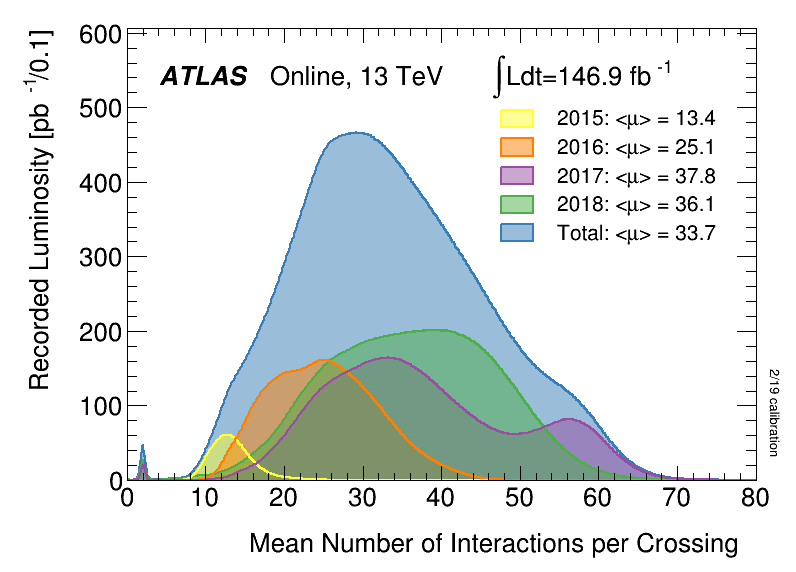
\includegraphics[width=0.5\linewidth]{images/mu_2015_2018.png} &
        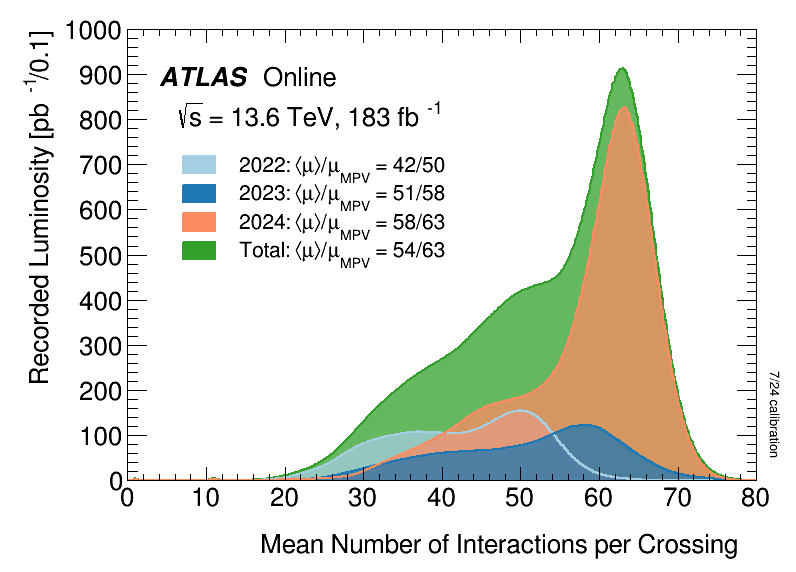
\includegraphics[width=0.5\linewidth]{images/mu_2022_2024.png} \\
        (a) & (b)  \\
    \end{tabular}
    \caption{(a) Distribution of mean number of interactions per bunch crossing in data recorded by the \acrshort{atlas} experiment at 13~TeV during Run 2~\cite{atlas:Run2lumi} and  (b) at 13.6~TeV during Run 3~\cite{atlas:Run2lumi} data-taking periods.}
    \label{fig:pileup}
    \end{figure}
%xxxxxxxxxxxxxxxxxxxxxxxxxxxxxxxxxxxxxxxxxxxxxxxxxxxxxx
\subsection*{LHC upgrade plans}
%xxxxxxxxxxxxxxxxxxxxxxxxxxxxxxxxxxxxxxxxxxxxxxxxxxxxxx

To further push the frontiers of high-energy physics and enhance the physics reach of the LHC programme, a major upgrade of the collider and its experiments is underway. The High-Luminosity LHC (HL-LHC) project~\cite{HLLHC} aims to increase the integrated luminosity delivered to the experiments by more than an order of magnitude, targeting up to 3000~fb$^{-1}$ of proton--proton collision data by the end of the next decade.

This increase in data volume will significantly improve the statistical precision of measurements of rare processes and enable detailed studies of the Higgs boson properties, electroweak interactions, and potential signals of physics beyond the Standard Model. In particular, the HL-LHC will allow for precise measurements of Higgs boson couplings, self-interactions, and rare decays, as well as the potential observation of extremely suppressed processes such as flavour-violating decays or double Higgs production.

Achieving the HL-LHC goals requires a broad range of upgrades to the accelerator complex and its associated infrastructure. Key improvements include the installation of new high-field superconducting quadrupole magnets near the interaction points, based on advanced Nb$_3$Sn technology~\cite{Mangiarotti:2770766}, which will allow for a reduction in the beams width, and consequently, an increase in luminosity. Additionally, new cryogenic and collimation systems will be implemented to handle the increased beam power and radiation levels.

On the experiment side, all main LHC experiments, including ATLAS, are undergoing substantial upgrades to handle the harsher conditions of HL-LHC operation. These include the development of new inner trackers with extended radiation hardness and granularity, the replacement of calorimeter and muon chamber readout electronics to support higher data rates, and a completely redesigned trigger and data acquisition system. The upgraded detectors must be capable of maintaining excellent performance in the presence of average pile-up levels exceeding $\langle\mu\rangle \sim 140$, more than a factor of two higher than those typically encountered during Run~3.

The HL-LHC project is expected to start operations by 2029, following the completion of the Long Shutdown 3 (LS3). It represents the next major milestone in the LHC physics programme, with the potential to open a new era of precision measurements and exploration of the unknown.


%++++++++++++++++++++++++++++++++++++++++++++++
\section{The ATLAS detector}
\label{sec:ATLAS}
%++++++++++++++++++++++++++++++++++++++++++++++

Having already outlined the design, physics programme and scientific goals of the LHC experiment, this section presents in detail each of the main components that make up the ATLAS detector.

ATLAS (A Toroidal LHC ApparatuS)~\cite{ATLAS:exp,ATLAS:1999uwa} is a general-purpose detector designed to explore a wide spectrum of physics phenomena, ranging from precision tests of the Standard Model to searches for new particles and interactions beyond it. It is the largest 
detector ever constructed for a collider experiment, with a cylindrical geometry approximately 44~m long, 25~m diameter, and weighing over 7000~tons. Its conception, design and construction were carried out by a global collaboration of more than 3000 scientists and engineers from around 180 institutions in nearly 40 countries.

Data-taking with ATLAS began in 2009, when the LHC first delivered proton-proton collisions. Since then, the detector has been instrumental in several landmark achievements, most notably the discovery of the Higgs boson in 2012. The ATLAS detector is composed of multiple subdetectors arranged in concentric layers 
around the interaction point. The cylindrical structure is closed by two end-caps, providing almost $4\pi$ coverage of the solid angle. An illustration of the ATLAS detector can be found in Figure~\ref{fig:ATLASdet}.

The different ATLAS subsystems are designed to measure the properties of different types of particles. In the innermost region, closest to the interaction point, the inner detector is built to record the properties of charged particles produced in the collisions. Their trajectories 
are bent by a 2~T magnetic fields produced by a superconducting solenoid. Then, the inner detector is surrounded by the calorimeter system which is in charge of measuring the energy of particles that can produce electromagnetic and hadronic showers in the detector. It is striped in a liquid argon electromagnetic calorimeter and a hadronic calorimeter composed by a scintillating barrel and liquid argon end-caps.
In the outermost region of the detector it is placed the muon spectrometer, devoted to the measurement of muons produced in the collision and which are bent by a 4~T magnetic field produced in this case by a toroidal magnet system.
The following sections describe the purpose and operating principles of these components in detail, as well as the forward detectors and the trigger and data acquisition system.

\begin{figure}[htbp]
    \centering
        \includegraphics[width=1\linewidth]{ATLAS-Experiment-Schematic-2022-Labels-People.png}
    \caption{Cut-away view of the Run~3 configuration of the \acrshort{ATLAS} detector indicating the locations of the larger detector sub-systems~\cite{Bianchi:2837191}.}
    \label{fig:ATLASdet}
\end{figure}

%xxxxxxxxxxxxxxxxxxxxxxxxxxxxxxxxxxxxxxxxxxxxxxxxxxxxxx
\subsection{Reference frames and coordinate system}
\label{sec:coordinates}
%xxxxxxxxxxxxxxxxxxxxxxxxxxxxxxxxxxxxxxxxxxxxxxxxxxxxxx

The ATLAS experiment adopts a right-handed coordinate system, centered at the nominal interaction point (IP) where the proton--proton collisions take place. The origin of the coordinate system lies at the geometrical center of the detector. The $z$-axis is defined along the beam pipe, pointing in the direction of the anti-clockwise beam. The $x$-axis points from the IP towards the center of the LHC ring, while the $y$-axis points upwards, 
completing a right-handed coordinate system. The transverse plane defined by $x$ and $y$ directions locate important observables like the transverse momentum ($p_{T}$) and the so-called missing transverse momentum ($E^{miss}_{T}$).

In addition to the Cartesian coordinates $(x, y, z)$, a cylindrical coordinate system is often used due to the symmetry of the detector. In this system, the transverse plane is defined by the coordinates $(r, \phi)$, where $r$ is the radial distance from the $z$-axis and $\phi$ is the azimuthal angle measured around the beam pipe. The longitudinal direction remains aligned with the $z$-axis.

To describe the polar angle of a particle’s trajectory, defining deviations from the beam direction, the rapidity $y$ is preferred over the polar angle $\theta$, as it is invariant under Lorentz boosts along the $z$-axis:
\begin{equation}
    y = \frac{1}{2}\ln{\frac{E+p_{Z}}{E-{p_{Z}}}},
\end{equation}
where E is the particle's energy and $p_{Z}$ the longitudinal component of its momentum. In the ultra-relativistic limit, this variable can be approximated by the so-called pseudorapidity, $\eta$, since the mass of most of final-state particles is mostly negligible against their momenta:
\begin{equation}
\eta = -\ln \tan \left( \frac{\theta}{2} \right).
\end{equation}
In this frame, if a particle is emmitted in the beam direction, $\theta \rightarrow 0º$, it would have assigned $\eta \rightarrow \infty$, while if it follows a direction perpendicular to the beam, $\theta = 90º$ corresponds to $\eta = 0$.
The angular distance between two objects in the detector is typically measured using the $\Delta R$ metric in the $(\eta, \phi)$ plane:
\begin{equation}
\Delta R = \sqrt{(\Delta \eta)^2 + (\Delta \phi)^2}.
\end{equation}

This coordinate convention is used throughout the analysis and the design of the detector subcomponents, as well as in reconstruction and identification algorithms for physics objects such as jets, leptons, and missing transverse energy. It is illustrated in Figure~\ref{fig:coord}.
\begin{figure}[htbp]
    \centering
        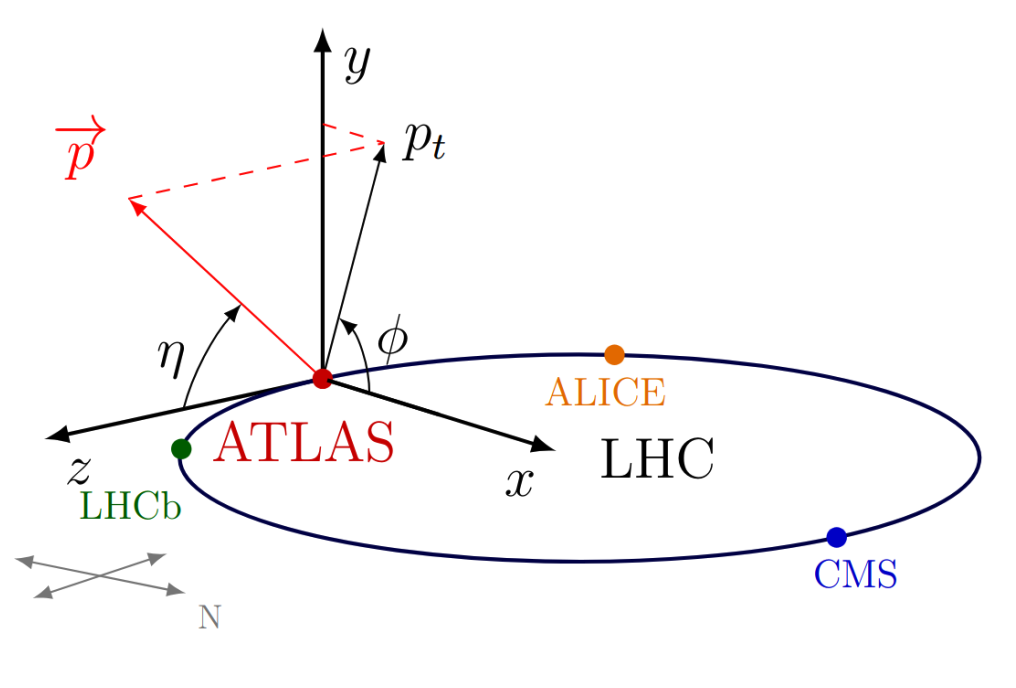
\includegraphics[width=0.7\linewidth]{ATLAS_coordinates.png}
    \caption{Illustration of the ATLAS coordinate system. Image obtained from Ref.~\cite{coordinates}.}
    \label{fig:coord}
\end{figure}

%xxxxxxxxxxxxxxxxxxxxxxxxxxxxxxxxxxxxxxxxxxxxxxxxxxxxxx
\subsection{Inner detector}
\label{sec:ID}
%xxxxxxxxxxxxxxxxxxxxxxxxxxxxxxxxxxxxxxxxxxxxxxxxxxxxxx


The Inner Detector (ID)~\cite{id1,id2} is the central tracking system of the ATLAS experiment and plays a fundamental role in the reconstruction of charged particles emerging from proton-proton collisions. It is the innermost component of the detector, positioned directly around the interaction point, and it is enclosed within a thin superconducting solenoid that generates a 2~T magnetic field parallel to the beam axis. This magnetic field bends the trajectory of charged particles in the $\phi$ direction, which allows the determination of their charge and momentum due to this curvature.

The ID is composed of three complementary subdetectors arranged in layers from the innermost to the outermost radii: the Pixel Detector, the Semiconductor Tracker (SCT), and the Transition Radiation Tracker (TRT). The Pixel and SCT systems are based on silicon technologies and are optimized for high spatial resolution and precision tracking, particularly near the primary vertex, which is the measured spatial location where the hard scattering of partons of interest in a given event took place. In contrast, the TRT is a gaseous detector made of straw tubes and is designed to extend the tracking capabilities at higher radii while also enhancing electron identification through the detection of transition radiation.

Together, these three subdetectors span a cylindrical volume of approximately 6.2~m in length and 2.1~m in diameter, and provide tracking coverage in the pseudorapidity range of $|\eta| < 2.5$. The layout of the ID is divided into a central barrel region ($|\eta| < 1.4$) and two symmetric endcap sections ($1.4 < |\eta| < 2.5$). As charged particles traverse the ID, they produce hits in the different layers, which are then used to reconstruct their trajectories with high efficiency and resolution. This track information is vital for identifying not only primary vertices, but other vertices that are displaced from the primary one and could originate from the decay of heavy-flavour hadrons that travels enough before decaying. This is clearly essential for tagging of these jets, and supporting particle identification algorithms throughout the ATLAS reconstruction chain, as will be explained in Chapter~\ref{chap:object_rec}.
An schematic view of the barrel section of the ID can be found in Figure~\ref{fig:id}.
\begin{figure}[htbp]
    \centering
        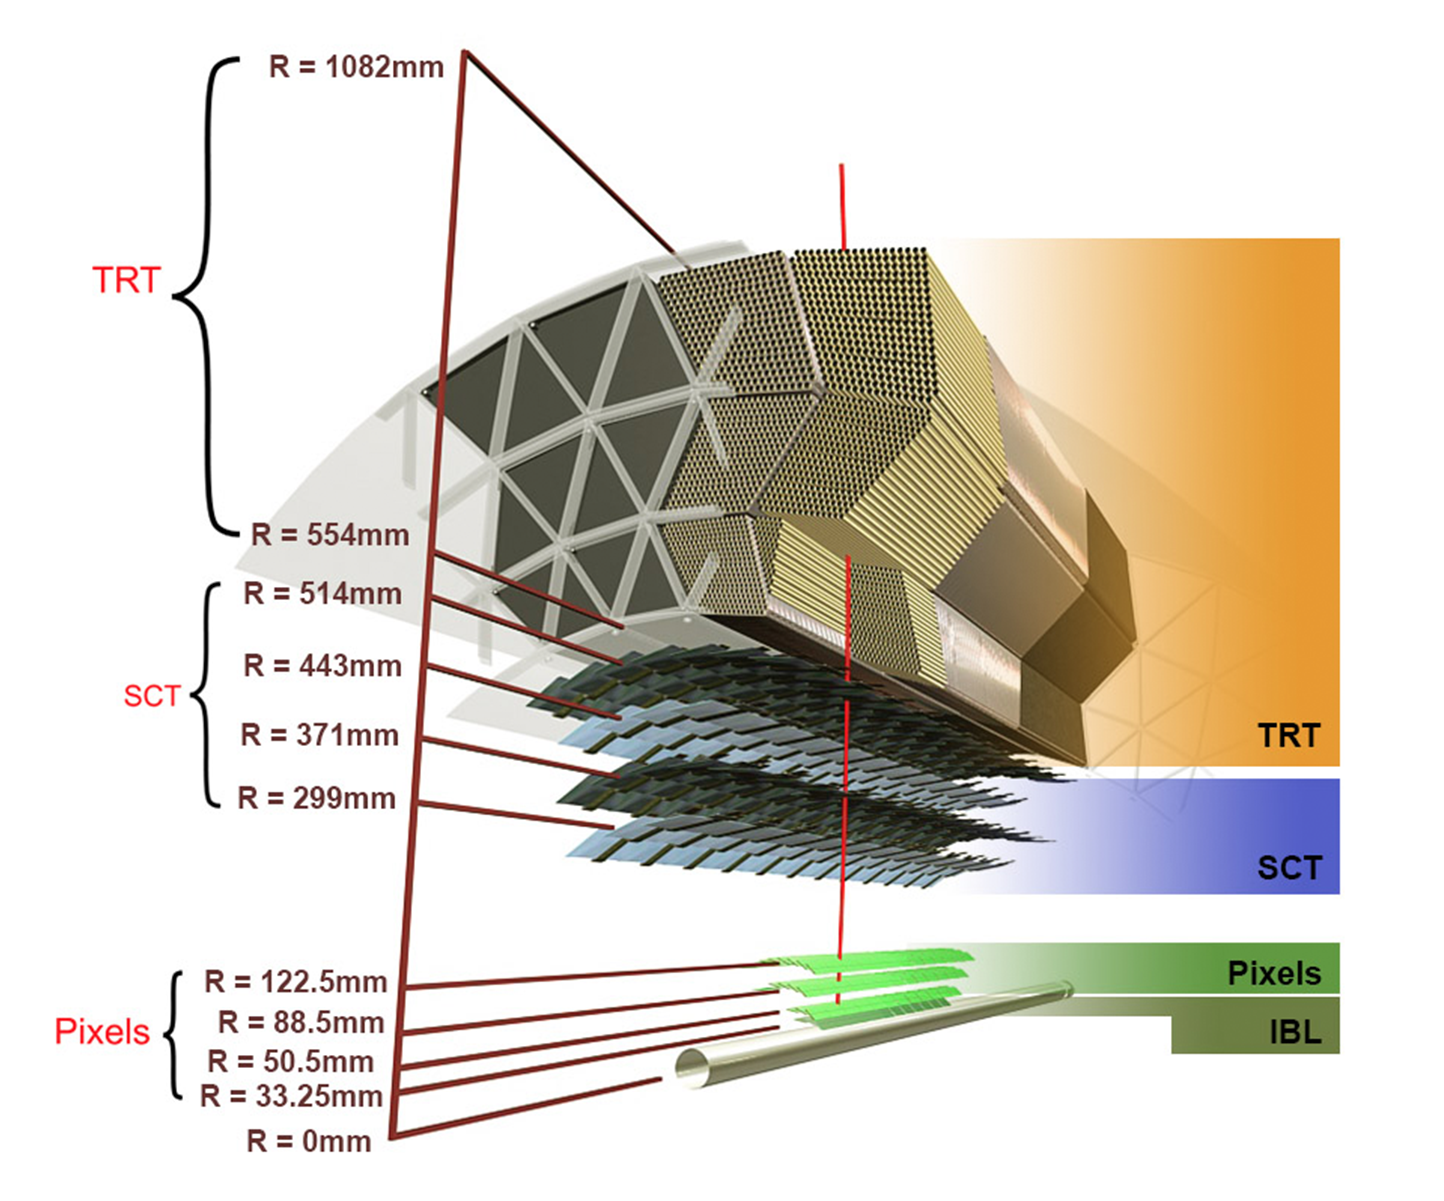
\includegraphics[width=0.7\linewidth]{ATLAS_id.png}
    \caption{Cutaway representation of the barrel section of the ATLAS inner detector. From the innermost to the outermost layers, it shows the pixel detector, the four cylindrical an concentrical layer of the SCR and the straw tubes characteristic of the TRT~\cite{Collaboration:2723878}.}
    \label{fig:id}
\end{figure}

\subsubsection*{Pixel detector}

The Pixel Detector is the innermost and most granular component of the ID. Its layout consists of three cylindrical layers of silicon pixel sensors in the barrel region, positioned at radial distances of 50.5, 88.5, and 122.5~mm, and three disks per endcap located at $z = \pm$495, 580, and 650~mm. The sensors in these layers have pixel sizes of $50 \times 400~\mu\text{m}^2$ and a thickness of 250~$\mu$m. This geometry yields a spatial resolution of about $10~\mu$m in the $r\text{--}\phi$ plane and $115~\mu$m in $z$ for the barrel region, and the opposite in the endcaps, where resolution is optimized along $z$.

In preparation for Run~2, an additional innermost layer known as the Insertable B-Layer (IBL)~\cite{IBL} was installed at a radius of 33.25~mm. The IBL significantly improved the impact parameter resolution, particularly for low-$p_{\mathrm{T}}$ tracks. It is composed of both planar and 3D silicon sensors with reduced pixel dimensions of $50 \times 250~\mu\text{m}^2$ and sensor thicknesses of 250~$\mu$m and 200~$\mu$m, respectively. The closer proximity of the IBL to the beamline and its finer segmentation improves its ability to separate primary and secondary vertices even under high occupancy conditions, which is crucial for the identification of jets originating from heavy-flavour quarks.

During Run~3, the Pixel Detector has been operating under increasingly harsh radiation environments and elevated levels of pile-up. These conditions challenge the performance and life-time of the system, especially the innermost layers. Dedicated calibration and alignment strategies, as well as enhanced readout electronics, are employed to preserve the resolution and efficiency of tracking throughout this demanding phase of operation.

\subsubsection*{Semiconductor Tracker (SCT)}

Outwards, the SCT subdetector follows the pixel one, consisting of four barrel layers and nine disks in each endcap, built with silicon microstrip modules. Each module includes two sensors, mounted back-to-back at a small stereo angle of 40 mrad, enabling precise 3D position reconstruction of $17$~$\mu$m resolution in the transverse plane and $580$~$\mu$m in the longitudinal direction. 
The SCT contains around 6 million readout channels.

\subsubsection*{Transition Radiation Tracker (TRT)}

The TRT is the outermost component of the Inner Detector and extends tracking capabilities up to $|\eta| < 2.0$, complementing the precise position measurements from the inner silicon detectors with additional points along the track path. The TRT also provides particle identification (PID) capabilities, particularly useful for electron-pion discrimination via detection of transition radiation photons.

It consists of a large number of thin straw tubes, 52,544 in the barrel region and 122,880 in the two endcaps, each with a diameter of 4~mm. These tubes are originally filled with a gas mixture of 70\% xenon, 27\% carbon dioxide, and 3\% oxygen. When a charged particle traverses a straw, it ionizes the gas along its path. A high negative voltage applied to the tube walls causes the liberated electrons to drift toward a central anode wire, producing a detectable signal. 

The TRT delivers a spatial resolution of approximately $130~\mu\text{m}$ in the $r\text{--}\phi$ plane and contributes on average about 30 measurement points per track, thus enhancing the momentum resolution and the track reconstruction efficiency, especially for high-$|\eta|$ regions where fewer silicon hits are available. Its ability to identify transition radiation, photons emitted by relativistic electrons crossing dielectric boundaries embedded in the tracker, provides an additional layer of particle identification crucial for several physics analyses.

During Run~3, it has been used an argon-based gas mixture in the entire barrel and part of the end-cap region to minimize xenon loss and ensure gas stability. Although this reduces the barrel's PID performance due to weaker transition radiation photon absorption, it still provides useful electron identification when combined with d$E$/d$x$ information. The end-cap PID performance remains largely preserved~\cite{ATLAS_run3}.

\vspace{-0.3}
At this stage it is worth noting that, ahead of Run 3, an important part of the read-out electronics in several sub-detectors were refurbished and optimised to withstand the higher data rates expected during this period. By the end of Run~3 the existing silicon trackers will be operating close to their radiation-tolerance limits, and the TRT will no longer be able to function under the nominal HL-LHC conditions. To preserve vertex-tagging and track-reconstruction performance, the entire Inner Detector will therefore be superseded by an all-silicon Inner Tracker (ITk). In addition, a High-Granularity Timing Detector will be installed in the forward region in order to match tracks with calorimeter clusters using precise time information, that is an essential tool for mitigating the extreme pile-up foreseen at the HL-LHC \cite{ATLAS:1502664}
%xxxxxxxxxxxxxxxxxxxxxxxxxxxxxxxxxxxxxxxxxxxxxxxxxxxxxx
\subsection{Calorimeters}
\label{sec:calo}
%xxxxxxxxxxxxxxxxxxxxxxxxxxxxxxxxxxxxxxxxxxxxxxxxxxxxxx
Moving outwards again, beyond the solenoid magnet containing the Inner Detector, we find the ATLAS calorimeter system~\cite{lar_tech,tile_tech}, which fully encloses the previously described 
components. Both types of calorimeters, electromagnetic and hadronic, cover a total range up to $|\eta| < 4.9$, allowing for the measurement of the energy of particles traversing them, 
as they are nominally designed to completely absorb the energy of most particles predicted by the \acrshort{sm}, 
except for muons and neutrinos. An schematic illustration of the ATLAS calorimeter system is shown in Figure~\ref{fig:cal}.
\begin{figure}[htbp]
    \centering
        \includegraphics[width=0.9\linewidth]{ATLAS_cal.jpg}
    \caption{Cutaway representation of the ATLAS calorimeter system and its main components~\cite{Collaboration:2723878}.}
    \label{fig:cal}
\end{figure}

%%%%%%%%%%%%%%%%%%%%%%%%%%%%%%%
\subsubsection{LAr electromagnetic calorimeter}
\label{sec:elelar}
%%%%%%%%%%%%%%%%%%%%%%%%%%%%%%%

The electromagnetic calorimeter (EM calorimeter) in the ATLAS detector is designed to precisely measure the energy of electrons and photons. It is based on a sampling technology that uses liquid argon (LAr) as the active medium and different metals (either tungsten, copper or lead) as the absorber material. This choice combines a high level of granularity with excellent linearity and radiation hardness, crucial for operation in the high-luminosity environment of the LHC.

The EM calorimeter is divided into three main regions: a barrel section covering the pseudorapidity range $|\eta| < 1.475$ (EMB), and two end-cap sections (EMEC) that extend the coverage up to $|\eta| = 3.2$. Each region is segmented longitudinally into three layers (plus a presampler), as can be seen in Figure~\ref{fig:LAr_EM}, optimizing the reconstruction of electromagnetic showers. The presampler layer is used to correct for energy loss in the material upstream of the calorimeter. The first layer features fine granularity in the $\eta$ direction ($\Delta\eta = 0.0031$), allowing for precise discrimination between single photons and the two close-by photons resulting from $\pi^0$ decays. The second layer collects most of the energy from electromagnetic showers and provides the primary energy measurement. The third layer corrects for energy leakage at high energies.

\begin{figure}[htbp]
    \centering
        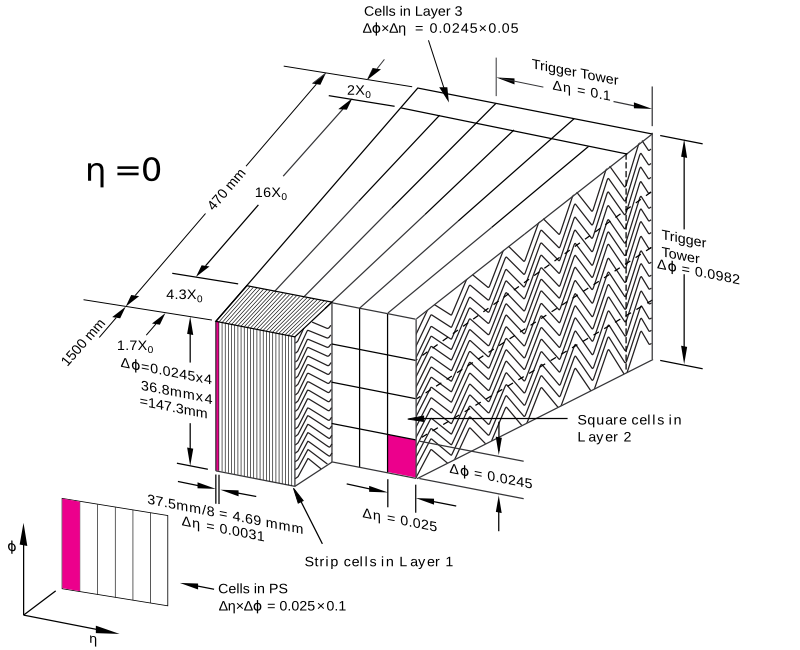
\includegraphics[width=0.8\linewidth]{LAr_EM.png}
    \caption{Schematic diagram of the cross-section of the LAr EM barrel calorimeter, including the presampler. The different granularity in $\eta$ and $\phi$ of the cells of each of the three layers is also shown~\cite{atlas:EM_LAr}}
    \label{fig:LAr_EM}
\end{figure}

The LAr calorimeter employs an accordion-shaped geometry in both the barrel and end-cap regions. This design ensures full azimuthal coverage without projective cracks, while maintaining uniform response and mechanical stability. The calorimeter modules are housed in cryostats filled with liquid argon, operating at a temperature of approximately 87~K. The readout cells are segmented into towers of size $\Delta\eta \times \Delta\phi = 0.025 \times 0.025$ in the second layer, which defines the granularity for standard electromagnetic object reconstruction.

The signal is induced by the ionization of the LAr by charged particles in the shower. Ionization electrons drift under a high-voltage electric field, and the resulting current is read out with high precision using fast, low-noise electronics, used to determine the energy deposited by the original particle that hit the detector. The typical energy resolution of the EM calorimeter is described by the expression:
\begin{equation}
\frac{\sigma_E}{E} = \frac{a}{\sqrt{E}} \oplus b \oplus \frac{c}{E},
\end{equation}
where $a$ represents the stochastic term (about $10\%$), $b$ the constant term (below $0.7\%$), and $c$ the noise term. The excellent resolution is essential for precision measurements such as the $H \rightarrow \gamma\gamma$ and $H \rightarrow ZZ^* \rightarrow 4\ell$ channels.

%%%%%%%%%%%%%%%%%%%%%%%%%%%%%%%
\subsubsection{LAr hadronic calorimeters}
\label{sec:elehad}
%%%%%%%%%%%%%%%%%%%%%%%%%%%%%%%

The hadronic calorimeter system complements the electromagnetic calorimeter by measuring the energy of hadrons. In the end-cap and forward regions, the hadronic calorimetry is provided by these LAr-based detectors: the Hadronic End-Cap Calorimeter (HEC) and the Forward Calorimeter (FCal). These systems are critical for reconstructing jets, missing transverse energy, and for identifying hadronically decaying $\tau$-leptons in the forward regions.

The HEC is positioned directly behind the EMEC and covers the pseudorapidity range $1.5 < |\eta| < 3.2$. It consists of copper plates as absorbers and uses liquid argon as the active medium. The copper-LAr combination ensures a compact structure with good radiation hardness and linearity. The HEC is segmented longitudinally into four layers and provides a depth of about 10 interaction lengths ($\lambda_0$) when combined with the electromagnetic calorimeter, enabling efficient hadronic shower containment. Each end-cap consists of two wheels: a front wheel (HEC1) constituted of 24 copper plates, and a rear wheel (HEC2) made of 16 copper plates.

The Forward Calorimeter (FCal) extends the coverage to $|\eta| < 4.9$ and is composed of three longitudinal modules: the first is electromagnetic, featuring copper absorbers, and the second and third are hadronic, and uses tungsten absorbers in order to reduce the lateral spread of the hadronic showers. The high-density design of the FCal is necessary to withstand the high particle flux and radiation levels encountered in the forward region. Due to its crucial role in reconstructing the forward energy flow, the FCal is also essential for pile-up suppression and missing transverse energy reconstruction.

Both HEC and FCal calorimeters operate within the same LAr cryostats as the electromagnetic sections, benefitting from the same stability and fast response. 

%%%%%%%%%%%%%%%%%%%%%%%%%%%%%%%
\subsubsection{Tile hadronic calorimeter}
\label{sec:tilecal}
%%%%%%%%%%%%%%%%%%%%%%%%%%%%%%%

The Tile Calorimeter (TileCal) is ATLAS's main hadronic calorimeter, constructed as a sampling calorimeter composed of alternating layers of plastic scintillator tiles (active material) and low-carbon steel absorber plates. Positioned around the LAr calorimeter, TileCal provides coverage in the pseudorapidity region $|\eta|<1.7$ and ensures containment of hadronic showers, limiting punch-through to the muon system with a total thickness of approximately 11~$\lambda_0$ at $\eta=0$.

TileCal consists of a central long barrel (LB) section ($|\eta|<1.0$, length of 5.8 m) and two extended barrel (EB) sections (EBA and EBC), each covering $0.8<|\eta|<1.7$ with a length of 2.6 m. Together with other calorimeters (HEC, FCal), TileCal achieves coverage up to $|\eta|<4.9$.

Each barrel segment is divided into 64 modules, featuring alternating 3 mm thick scintillator tiles and 14 mm thick steel absorbers along the beam axis. The scintillator tiles, arranged radially in 11 rows, generate scintillation light upon particle interaction. Wavelength-shifting (WLS) fibers collect and shift this light to longer wavelengths, guiding it to photomultiplier tubes (PMTs) at the module's outer radius, enabling efficient and hermetic readout.

The calorimeter modules are segmented into three longitudinal layers: layers A, BC, and D in the LB (1.5, 4.1, and 1.8 $\lambda_0$, respectively) and layers A, B, and D in the EB (1.5, 2.6, and 3.3 $\lambda_0$, respectively). Cells in these layers have granularity of $\Delta\eta \times \Delta\phi=0.1\times0.1$ for inner layers and $0.2\times0.1$ for outer layers.

Additionally, gap scintillator cells (E1-E4) were installed between TileCal and LAr to correct for energy losses and enhance performance. The Minimum-Bias Trigger Scintillators (MBTs), also read out by TileCal electronics, provide coverage in $2.08<|\eta|<3.86$ for triggering purposes. Overall, TileCal incorporates 9852 readout channels, covering 5182 cells.

Figure~\ref{fig:cal_resum} shows an schematic view of the readout geometry of all the calorimeter systems in the $r$--$z$ space, showing the different $\eta$ ranges covered by them.
\begin{figure}[htbp]
    \centering
        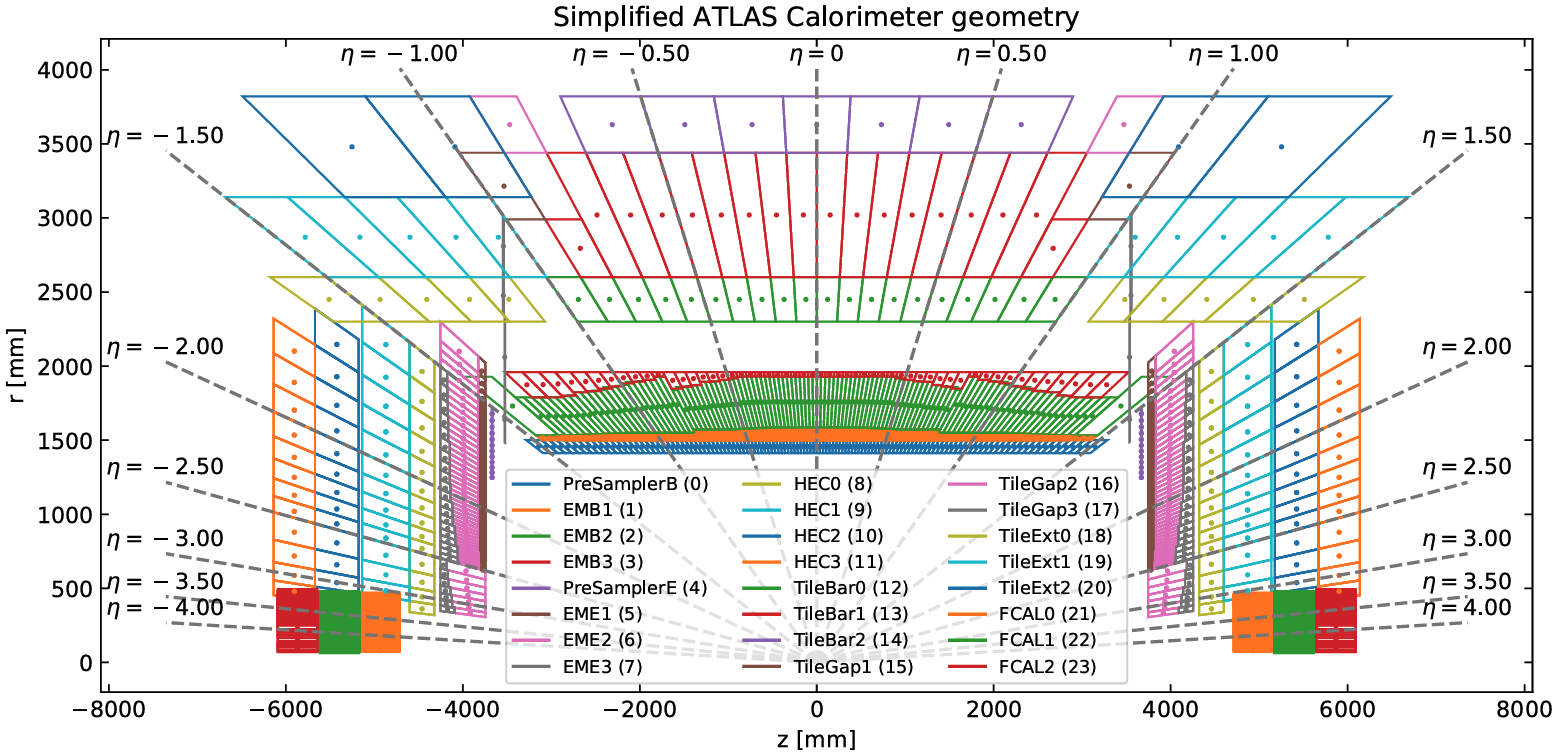
\includegraphics[width=0.9\linewidth]{cal_readout_ATLAS.png}
    \caption{Visualization of the ATLAS calorimeter readout geometry. The three subsystems, Tile, Liquid Argon and the Forward calorimeters, are shown~\cite{Gessinger:2752944}.}
    \label{fig:cal_resum}
\end{figure}

\vspace{-0.3}

Additional upgrades have also been implemented in the ATLAS calorimeter electronics to meet Run-3 conditions and to prepare for the forthcoming HL-LHC era, mirroring the improvements made to the Inner Detector and ensuring compatibility with the new trigger architecture. Both the Liquid-Argon and Tile Calorimeters have refurbished their on-detector and off-detector read-out chains; in TileCal specifically, new scintillating cryostat counters and renewed Minimum-Bias Trigger Scintillators have been installed for Run 3, enhancing electron-energy resolution and improving luminosity monitoring.

%xxxxxxxxxxxxxxxxxxxxxxxxxxxxxxxxxxxxxxxxxxxxxxxxxxxxxx
\subsection{Muon spectrometer}
\label{sec:muon}
%xxxxxxxxxxxxxxxxxxxxxxxxxxxxxxxxxxxxxxxxxxxxxxxxxxxxxx


Figure~\ref{fig:ms_atlas} shows the outermost subsystem of ATLAS, known as the Muon Spectrometer (MS)~\cite{mu_tech}. The MS is responsible for identifying muons, particles capable of traversing the calorimetric system with minimal energy loss. It comprises precision tracking chambers and fast-response trigger detectors embedded in a magnetic field of approximately 0.5~T in the barrel and 1.0~T in the end-cap regions, bending the trajectories of muons and enabling precise momentum measurement.

The MS includes four detector technologies totaling over one million readout channels. A schematic view of the subsystem is shown in Figure~\ref{fig:atlas_muon}, without including the New Small Wheel sector yet, implemented for Run~3. Two separate detector systems facilitate initial trigger decisions. Resistive Plate Chambers (RPCs) are used in the barrel region ($|\eta| < 1.05$), providing measurements with a resolution of about 10~mm in both longitudinal and transverse directions. In the end-cap region ($1.05 < |\eta| < 2.4$), Thin Gap Chambers (TGCs) handle higher background rates with wire separation of 1.8~mm and positional resolution around 5~mm. The RPC and TGC detectors primarily function as triggering components due to their fast response times.

Precision muon tracking relies mainly on Monitored Drift Tubes (MDTs), installed in both barrel and end-cap regions, covering the range $|\eta| < 2.7$ and offering high positional accuracy (approximately 35~µm per chamber). Cathode Strip Chambers (CSCs), multi-wire proportional chambers providing high rate capability and excellent time resolution (4~ns), are employed in the forward region ($2.0 < |\eta| < 2.7$). MDTs and CSCs are critical for accurately reconstructing muon trajectories.

For Run~3, the MS underwent significant upgrades, including the replacement of the forward muon-tracking region (known as the small wheel) with the New Small Wheel (NSW)~\cite{nsw_tech}. The NSW consists of two large 100-tonne detectors located at each end of ATLAS, each 10 metres in diameter and segmented into 16 sectors. The NSW employs advanced detector technologies such as Micromegas (MM) and small-strip Thin Gap Chambers (sTGC), capable of simultaneous precision tracking and triggering. Each wheel contains two layers of MM and sTGC chambers, resulting in four measurement planes for improved tracking accuracy and more than 2 million readout channels.
s
Moreover, despite being primarily designed to detect muons, the MS occasionally detects punch-through jets, hadronic jets that are not entirely absorbed by the calorimeters and reach the MS. The upgraded configuration of the MS, particularly with the addition of the NSW, significantly enhances ATLAS' capabilities in terms of tracking precision and trigger efficiency, essential for the high luminosity and challenging conditions expected during Run-3 and beyond.

Furthermore and aiming HL-LHC era, The Muon detectors will install new chambers in the barrel (RPCs and MDTs), replace the TGCs in the gap between the barrel and the end-caps and upgrade the readout electronics for the already installed RPCs, TGCs and MDTs to make them fully compatible with the trigger architecture.

\begin{figure}[htbp]
    \centering
        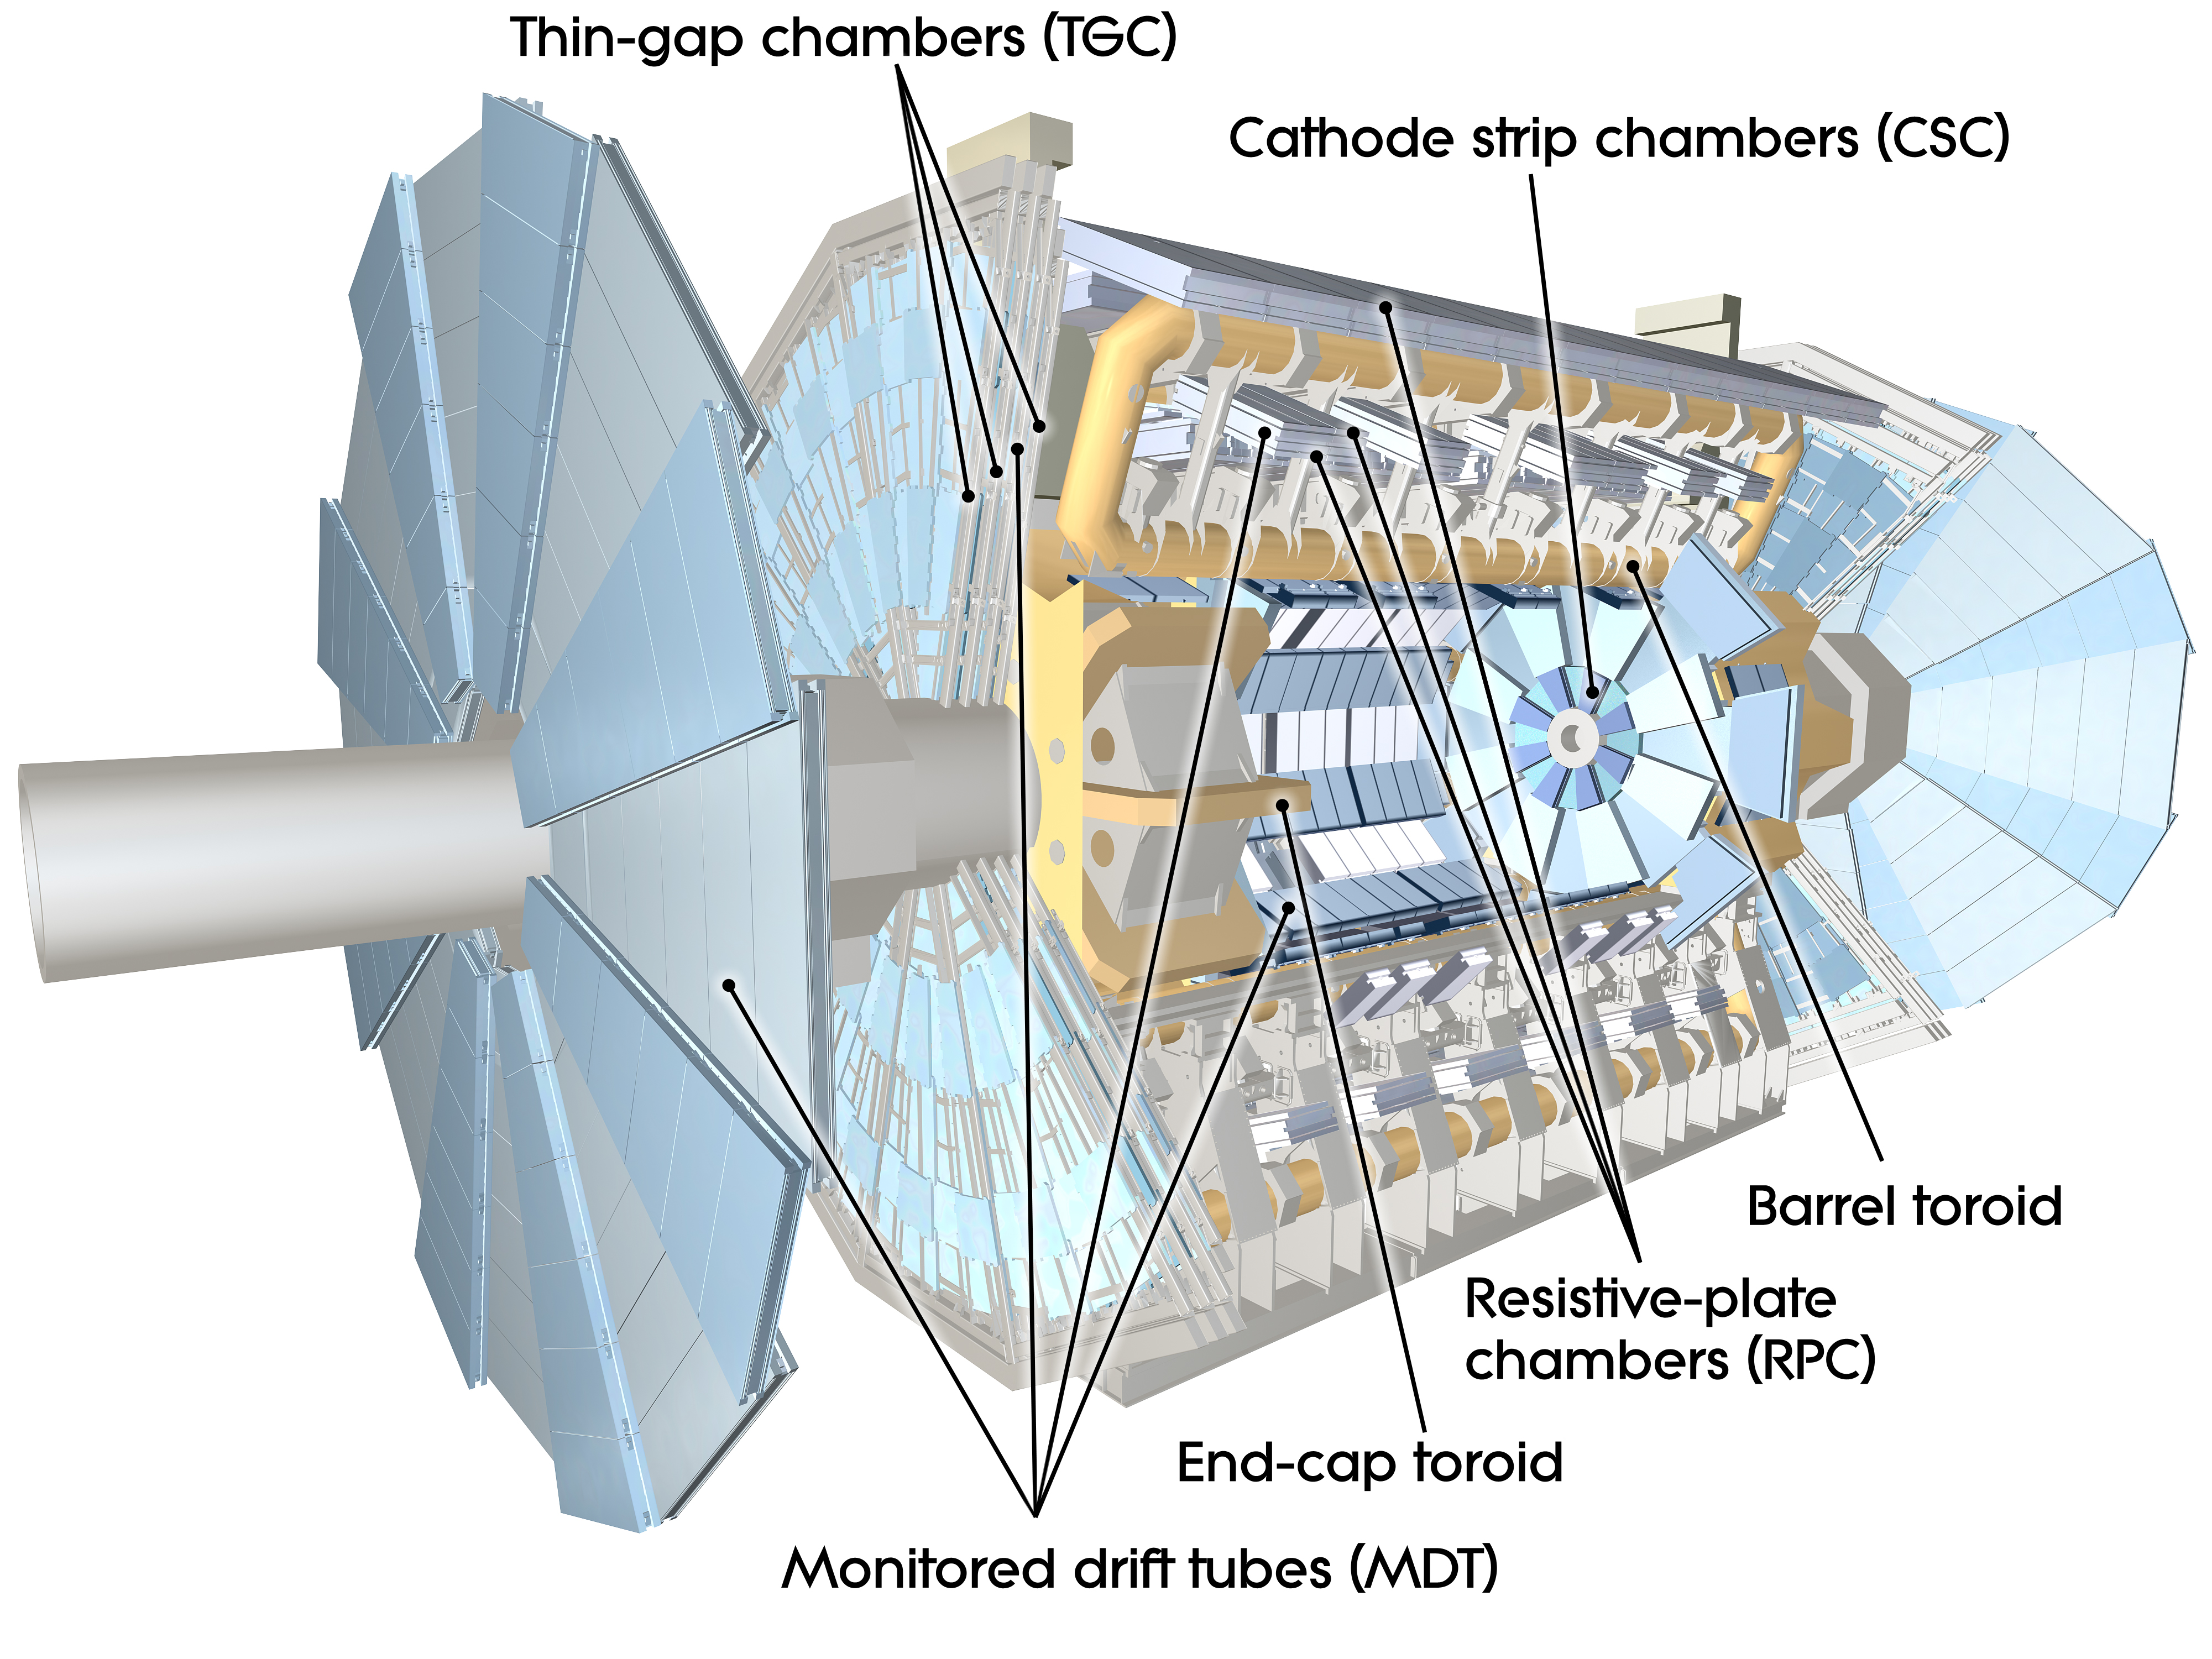
\includegraphics[width=0.9\linewidth]{ms_atlas.jpg}
    \caption{Cutaway representation of the ATLAS Muon Spectrometer~\cite{Bianchi:2837191}.}
    \label{fig:ms_atlas}
\end{figure}

%xxxxxxxxxxxxxxxxxxxxxxxxxxxxxxxxxxxxxxxxxxxxxxxxxxxxxx
\subsection{Forward detectors}
\label{sec:fwd}
%xxxxxxxxxxxxxxxxxxxxxxxxxxxxxxxxxxxxxxxxxxxxxxxxxxxxxx

Beyond the main subsystems listed above, ATLAS employs four compact forward subsystems covering the remaining region of the detector $(|\eta| > 5)$.
LUCID~\cite{Jenni:721908} (LUminosity Cherenkov Integrating Detector), situated $\pm17$ m from the interaction point, samples inelastic proton–proton interactions at very small angles and provides the experiment’s primary online and offline relative-luminosity measurement.  
LUCID is calibrated thanks to ALFA~\cite{Khalek_2016} (Absolute Luminosity For ATLAS), positioned inside Roman-pot stations $\pm240$ m from the IP, consists of scintillating-fibre tracking modules that can approach the beam to within $\sim\!1$ mm, enabling precise absolute-luminosity determinations and studies of elastic scattering.  
The AFP~\cite{Adamczyk:2015cjy} (ATLAS Forward Proton detector) was the last addition, located at 204 and 217 meters from the interaction point of both sides of the detector and aiming to extend the ATLAS physics reach by trying to tag very forward protons and enabling the observation of different processes where one of the two protons remains untouched.
Finally, the Zero Degree Calorimeter (ZDC)~\cite{Jenni:1009649}, installed $\pm140$ m from the IP, is built from alternating tungsten plates and quartz rods.  Covering $|\eta| > 8.3$, it detects neutral particles at zero degrees and is crucial for centrality measurements in heavy-ion collisions.

%xxxxxxxxxxxxxxxxxxxxxxxxxxxxxxxxxxxxxxxxxxxxxxxxxxxxxx
\subsection{Trigger, Data Acquisition and Detector Control Systems}
\label{sec:trigger}
%xxxxxxxxxxxxxxxxxxxxxxxxxxxxxxxxxxxxxxxxxxxxxxxxxxxxxx
One of the most demanding challenges for an experiment such as ATLAS at the LHC is to devise an efficient strategy for handling the enormous volume of data recorded in the tiny interval that follows each proton–proton collision. During routine LHC operation, proton bunches cross every 25 ns, yielding a raw collision rate of 40 MHz. Since each interaction produces thousands of particles,together with their consequent showers, a single fully digitised ATLAS event occupies roughly 1.5 MB, which would translate into a data stream of about 60 TB s$^{-1}$. Practical bandwidth and storage constraints therefore make it impossible to archive every event, and, in any case, the majority are not relevant to the core physics goals of the experiment. To curb this flood while retaining the maximum amount of useful information, ATLAS employs a dedicated trigger system~\cite{trigger_run2}. During Run 2 the trigger chain comprised two levels: a hardware–based Level-1 (L1) trigger, followed by a software–based High-Level Trigger (HLT). A schematic overview of the ATLAS Trigger and Data-Acquisition (TDAQ) system for Run 2 is shown in Figure~\ref{fig:trigger_system}.
\begin{figure}[htbp]
    \centering
        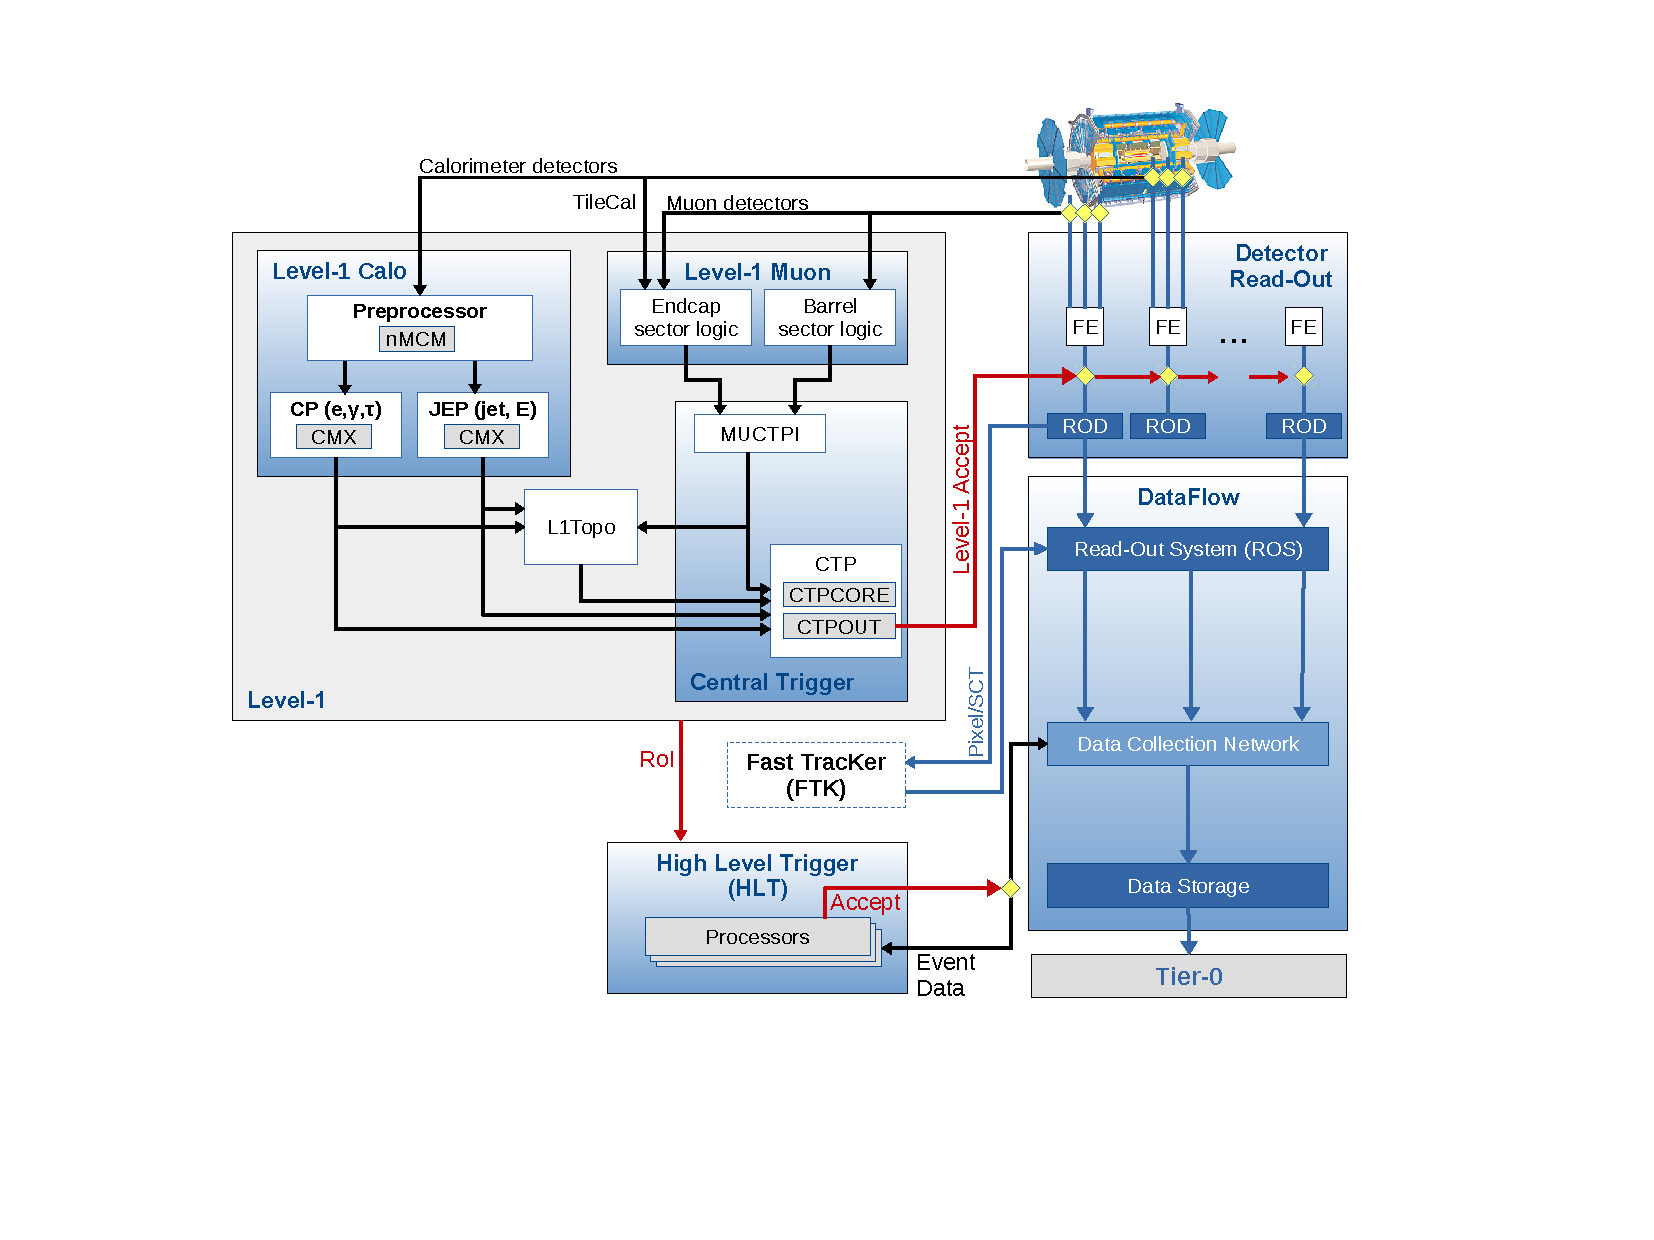
\includegraphics[width=0.9\linewidth]{tdaq-run2.pdf}
    \caption{Schematic of the ATLAS Trigger and Data Acquisition system in Run 2 with specific focus given to the components of the L1 Trigger system~\cite{atlas_daq_run2}.}
    \label{fig:trigger_system}
\end{figure}

The Level-1 trigger is a hardware-based system that cuts the raw 40 MHz collision rate down to about 100 kHz, operating with an exceptionally short latency of roughly 2.5 µs thanks to purpose-built custom and commercial electronics. The front-end electronics of every sub-detector store data in on-chip pipeline memories at the full 40 MHz bunch-crossing frequency. These buffers keep the digitised samples for ∼25 µs, that is the fixed window within which the L1 decision must be issued. That decision relies exclusively on information from the calorimeters and the muon spectrometer.

The L1 Calorimeter (L1Calo) trigger uses coarsened calorimeter read-outs (trigger towers) to locate regions of high energy deposition, i.e.\ regions of interest (RoIs). The L1 Muon (L1Muon) trigger exploits hits in the RPCs and TGCs to flag muon candidates, estimate their transverse momentum, and assign them to the correct bunch crossing. Outputs from L1Calo and L1Muon are merged in the Central Trigger Processor (CTP), which delivers the final verdict. If an event is accepted (an L1-Accept, or L1A), a signal is sent back to the front-end electronics so that the complete data corresponding to that bunch crossing can be read out from the pipeline memories. As noted above, the maximum L1A rate in ATLAS is 100 kHz.

The events accepted at Level-1 are first formatted by the sub-detector Read-Out Drivers (RODs) and then forwarded to the software-based High-Level Trigger (HLT). Running on a large computer farm, the HLT performs a rapid, partial reconstruction—tracking, charged-particle and jet identification (including $b$-jets), and a first estimate of the missing transverse momentum, throttling the event stream from \SI{100}{\kilo\hertz} to roughly \SI{1}{\kilo\hertz}. Events that satisfy these online selections are written to permanent storage and transmitted to CERN’s Tier-0 centre for full offline reconstruction. While awaiting the HLT verdict, the corresponding data fragments remain buffered in the Read-Out System (ROS).

During Long Shutdown 2 (LS2, between Run~2 and Run~3) the Phase-I upgrade preserved the two-level architecture while introducing a suite of crucial improvements. A fully digital L1Calo trigger path now feeds three FPGA-based feature extractors: eFEX for electrons and photons, jFEX for jets and missing transverse energy, and gFEX for global event variables. It uses super-cell granularity as fine as $\Delta\eta\times\Delta\phi = 0.025\times0.025$. In the forward region $(1.3<|\eta|<2.4)$ the newly installed New Small Wheels provide high-resolution muon trigger primitives, tightening transverse-momentum thresholds and cutting fake rates. The refurbished Level-1 Topological Processor exploits the finer calorimeter and muon inputs to impose angular, invariant-mass and transverse-mass selections in hardware. At the second stage, the HLT farm now runs on expanded computing resources, maintaining an output of roughly 3 kHz at an average event size of about 2.1 MB.

The Phase-II TDAQ upgrade, developed for the new conditions that will be delivered by HL-LHC, therefore foresees a two-stage hardware trigger in which an initial Level-0 decision accepts events at roughly \SI{1}{\mega\hertz}, followed by a refined Level-1 selection that throttles the rate to about \SI{400}{\kilo\hertz}. Both stages will exploit full-granularity calorimeter read-outs together with prompt track information from the new ITk. The latency budget will be stretched to $\sim!\SI{10}{\micro\second}$, and a trigger-less streaming DAQ is foreseen, capable of digesting data throughputs in excess of \SI{5}{\tera\byte\per\second}. An enlarged processing farm, augmented with hardware accelerators such as FPGAs and GPUs, will then filter the stream down to a sustainable output of \SIrange{10}{15}{\kilo\hertz} for permanent storage. Collectively, these upgrades will preserve and probably extend the experiment’s physics reach in the demanding high-pile-up environment of the HL-LHC.

\subsubsection*{Detector Control Systems}
A smooth dialogue between all ATLAS subsystems and the technical infrastructure that steers them is essential for reliable detector operation and data flow. This coordination is handled by the Detector Control System (DCS)~\cite{atlas_DCS}, which provides a unified interface for operators and continuously monitors voltages, temperatures, gas flows, and countless other parameters. Whenever an abnormal condition is detected, the DCS automatically issues alarms, attempts corrective actions where possible, and guides shifters through any manual interventions required. In addition, the DCS exchanges status flags with the DAQ so that data taking proceeds only when all components are in a safe, ready state, and it brokers communication among subsystems that are controlled independently.

\subsubsection*{The LHC computer grid}

To explain how the events accepted by the trigger are eventually processed, one must introduce The Worldwide LHC Computing Grid (WLCG)~\cite{Bird:1695401}, which is a global, tiered infrastructure that stores, distributes and processes the multi-petabyte data stream produced by the LHC experiments.  Data first reach Tier-0 at CERN, where the raw 40 MHz detector output is buffered, reconstructed and replicated; CERN then distributes this primary dataset to thirteen Tier-1 centres on three continents for large-scale reprocessing and long-term archival. Roughly 170 Tier-2 sites (university and regional clusters) supply the bulk of CPU for user analyses and Monte-Carlo production, while countless local Tier-3 farms serve individual groups.  
Today the WLCG federates $\sim$1.4 million CPU cores and $\sim$1.5 EB of disk and tape across 42 countries, sustaining average data‐transfer rates above 260 GB s$^{-1}$ and executing in excess of two million grid jobs daily.  This distributed model enables more than 12 000 physicists to access ATLAS data quasi-real-time, making large-scale analysis feasible without centralised super-computing resources.

%-------------------------------------------------------------------------------

%-------------------------------------------------------------------------------
\chapter{Data and simulated samples}
\label{chap:dataset}
\newcommand{\MG}{\textsc{madgraph5}\xspace}
\newcommand{\MCNLO}{\textsc{mc@nlo}\xspace}
\newcommand{\aMCNLO}{\textsc{amc@nlo}\xspace}
\newcommand{\madgraph}{\textsc{madgraph5\_amc@nlo}\xspace}
\newcommand{\sherpa}{\textsc{sherpa}\xspace}
\newcommand{\OPENLOOPS}{\textsc{openloops}\xspace}
\newcommand{\powheg}{\textsc{powheg}\xspace}
\newcommand{\powhegbox}{\textsc{powheg-Box}\xspace}
\newcommand{\pythia}{\textsc{pythia}\xspace}
\newcommand{\herwig}{\textsc{herwig}\xspace}
\newcommand{\FxFx}{\textsc{FxFx}\xspace}
\newcommand{\MEPSNLO}{\textsc{MePs@NLO}\xspace}
\newcommand{\UNLOPS}{\textsc{UNLOPS}\xspace}
\newcommand{\MiNLO}{\textsc{MiNLO}\xspace}
\newcommand{\MADSPIN}{\textsc{MadSpin}\xspace}
\newcommand{\geant}{\textsc{Geant4}\xspace}
\newcommand{\afast}{\textsc{AtlFast-II}\xspace}
\newcommand{\evtgen}{\textsc{EvtGen}\xspace}
\newcommand{\toppp}{\textsc{Top}$_{++}$\xspace}
\newcommand{\COMIX}{\textsc{Comix}\xspace}
\newcommand{\PDFLHC}{\textsc{PDF4LHC}\xspace}
\newcommand{\tth}{\ensuremath{t\bar{t}H}\xspace}
\newcommand{\ctdiez}{\textsc{CT10NLO}\xspace}

\section{Proton-Proton event simulation}
\label{sec:event}

In this section, the modeling of proton-proton collisions occurring at the LHC is presented, which comprises several stages~\cite{BUCKLEY2011145}.
Firstly, the production cross-section for the hard scattering introduced previously in Section~\ref{subsec:proton} is calculated, describing the interactions between the partons that compose the incoming protons.
This is followed by parton showering, where gluon emissions and parton splitting are simulated. The next step involves hadronization, where resulting partons combine to form color-neutral hadrons, which subsequently decay along with other unstable particles. Additionally, the modeling of pile-up and underlying events, originating from multiple simultaneous proton interactions beyond the primary scattering within the same bunch crossing, is included.
Finally, events undergo detector simulation, digitization, and the same reconstruction algorithms used for real data, ensuring a realistic representation of experimental conditions.
Figure~\ref{fig:pdfs} illustrates the aforementioned steps involved in simulating a proton-proton collision.
\begin{figure}[htbp]
    \centering
    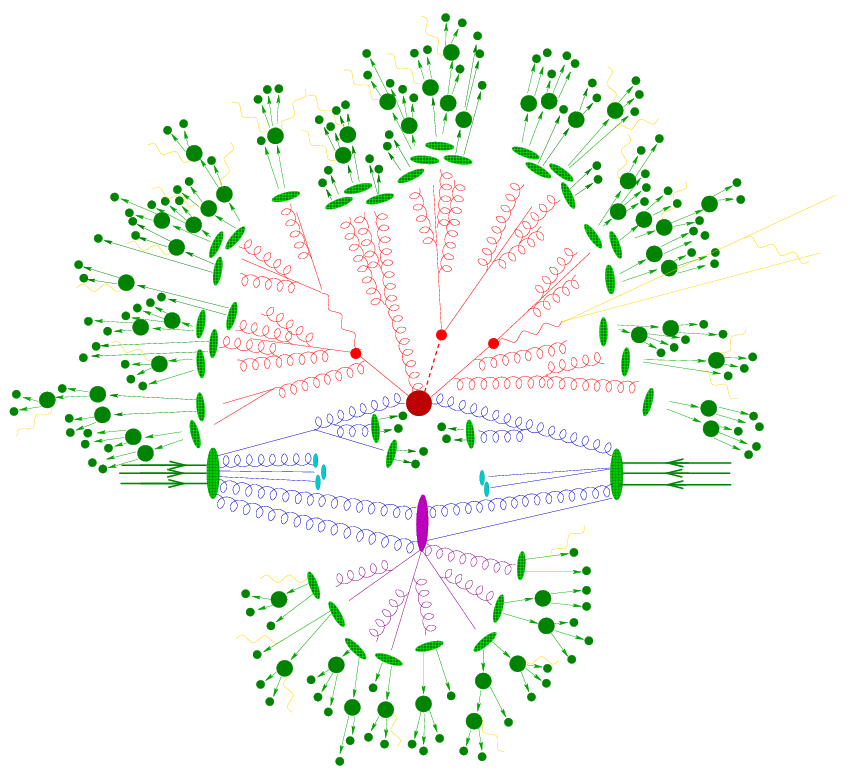
\includegraphics[width=0.9\textwidth]{images/atlas_pp_sim.png}
    \caption{Representation of components relevant for simulating a proton-proton collision event containing all the factorised stages, excluding pile-up~\cite{Gleisberg_2009}. The central red blob represents the hard-scattering of incident protons,
    while in blue it shows the initial partons that contributed. Additional hard QCD radiation, outgoing partons and their decays are also represented in red. In light green ellipses it is represented the hadronization of final state partons, while the decay
    of the resulting hadrons is represented by dark green regions with arrows. The partons that did not participate in the primary interaction conform the underlying event, in purple. In yellow one can find the photon radiation, that can occur at any stage.}
    \label{fig:pdfs}
  \end{figure}

\subsection{Matrix element and parton showers}
\label{subsec:parton_shower}
Given the large momentum transfer involved in the hard scattering processes at the LHC, the partonic cross-sections can be computed using perturbative QCD. In this framework, partons may radiate additional gluons and split into quarks, which in turn can emit yet more radiation both in the initial and final states. Computing the full cross-section ($\hat{\sigma})$ therefore requires summing over all possible quark/gluon emissions, which can be expressed as the perturbative expansion:
\begin{equation}
\hat{\sigma}(ij\rightarrow X) = \sum_{n=0}^{\infty}\int d\Phi_{X+n}\abs{\sum_{k=0}^{\infty}|\mathcal{M}_{X+n}^{^{(k)}}}|^2,
\end{equation}
being $\mathcal{M}_{X+n}^{^{(k)}}$ the matrix element for the process $ij \rightarrow X + n$, with $n$ the number of additional partons produced in the final state, $k$ the number of included virtual loops, and $d\Phi_{X+n}$ the phase space element for this process.
The calculation at LO only includes tree level matrix elements so it would correspond to $n=0$ and $k=0$. If the process involves the production of $N$ partons in the final state, then in this case the LO calculation for the process $ij \rightarrow X+N$ will involve $n=N$ and $k=0$.
In the same way, a matrix element calculation with $k + n = m$ is referred to as a calculation at $\text{N}^{\text{m}}$LO, for $ij \rightarrow X$.

This is how the cross-sections are calculated precisely for such scattering processes. However, when too many partons appear in the final state the computation becomes prohibitively expensive, so the matrix elements are evaluated only up to a certain order in the strong coupling constant
 $\alpha_{s}$ (see Eq.~\ref{running}), and the remainder is approximated via the parton-showering algorithm, where the showering is simulated using approximate matrix elements~\cite{FOX1980285}.

%%Because parton emissions span a wide range of energy scales, the phase space accessible to a parton-shower algorithm inevitably overlaps with that already covered by higher-multiplicity matrix elements. If left untreated, this overlap would double-count contributions and decrease the accuracy of cross-section and jet-multiplicity predictions, especially when an energetic, wide-angle emission converts an n-jet configuration into an (n + 1)-jet one.
%%Matching and merging prescriptions resolve the overlap by defining, event-by-event, which emissions originate from the fixed-order calculation and which from the shower. Slicing techniques introduce a matching scale: high-pT, large-angle partons are described by multi-leg matrix elements, while softer or more collinear radiation is delegated to the shower, preserving leading-logarithmic accuracy without duplication. Widely used implementations include 
%%the geometrical MLM~\cite{MANGANO2002343} algorithm and the CKKW~\cite{Catani_2001} schemes, which re-weight matrix elements and constrain subsequent showering; their next-to-leading-order extension is known as FxFx~\cite{Frederix_2012}. By combining samples of increasing jet multiplicity under these rules, one obtains inclusive event samples that smoothly interpolate between the hard and soft regimes.
Matching and merging schemes prevent double counting between high-multiplicity matrix elements and the parton shower by assigning emissions above a chosen matching scale to fixed-order calculations and relegating softer or collinear radiation to the shower. Widely used approaches, such as the MLM algorithm~\cite{MANGANO2002343} and CKKW schemes~\cite{Catani_2001} with their NLO extension FxFx~\cite{Frederix_2012}, combine tree-level multileg samples
of increasing jet multiplicity with parton showers to produce inclusive event samples that smoothly interpolate between hard, wide-angle emissions and soft, collinear radiation.

\subsection*{Hadronization}
\label{subsec:Hadronization}

Below the perturbative cutoff of order 1 GeV, parton showering hands off to non-perturbative hadronization, during which coloured partons (each carrying definite momentum, flavour and colour) are clustered into colour-neutral hadrons. Phenomenological models such as the Lund string model or the cluster model take over here.

In the Lund string model~\cite{ANDERSSON198331} the colour field between a quark and an antiquark is treated as a relativistic string whose potential energy rises with separation; when that energy exceeds the mass of a new $q\bar{q}$ pair the string breaks, repeatedly creating additional pairs until all energy is exhausted, with hadron momenta drawn from an empirical fragmentation function. 
The cluster model~\cite{Winter_2004} instead splits each final-state gluon into a $q\bar{q}$ pair and groups them into colour-singlet clusters; those clusters then undergo a cascade of decays, or directly fragment, until only stable hadrons remain.

\subsection*{Pile-up and underlying event}
\label{subsec:Pile}

All activity and interactions occurring in a proton-proton collision beyond the primary hard scattering must also be modelled; these are referred to as the underlying event and pile-up backgrounds, as discussed in Section~\ref{sec:LHC}. 
In the case of the underlying event, the soft interactions between partons are mainly described using phenomenological models, given their non-perturbative nature. When considering pile-up, one must simulate the additional proton-proton interactions that occur alongside the hard scattering, arising from nearby bunch crossings or even from protons interacting with beam-pipe or detector components.

Each of these effects is generated separately and then overlaid onto the hard-scattering event before passing the combined event through the full detector simulation.



\section{Detector response simulation}
\label{sec:Detector}

The raw collision data recorded by ATLAS arise solely from the interactions of final-state particles with the various subdetectors (see Section~\ref{sec:ATLAS}). To compare our Monte Carlo predictions with real data, each simulated event is propagated through a detailed detector model and reconstruct it identically to the collision data.  This full detector simulation is performed with the \textsc{Geant4} toolkit~\cite{AGOSTINELLI2003250}, which tracks particles through the precise geometry of every ATLAS subsystem, simulates their electromagnetic and hadronic interactions, and converts energy deposits and tracks into digitized detector signals.

For maximum accuracy one employs the “Full Simulation” procedure in which \textsc{Geant4} processes the complete ATLAS geometry.  However, calorimeter showers dominate the CPU cost, consuming nearly 90\% of the resources.  To speed up large-scale productions, the \textsc{AtlFast-II} fast-simulation simplified framework~\cite{Edmonds:1091969,ATLAS:1300517} applies parametrized responses for both the inner detector and calorimeters, reducing computing time by an order of magnitude.  Lastly, all simulations incorporate the actual detector conditions in force at the time of production: dead channels, electronic noise, alignment shifts, and calibration constants. Therefore the simulated events can always contain some mismatch with the real data, since the conditions of the detector change constantly during the data taking.


\section{Monte Carlo simulation generators}
\label{sec:mc}
Monte Carlo generators are basically software tools that use pseudorandom numbers to reproduce predicted kinematic distributions and event dynamics for a given physics process according to a theoretical model such as the SM.  They fall into two broad classes: general-purpose generators, which reproduce the entire chain of event generation (hard scattering, parton showering, hadronization, etc.), and more specialized codes that excel at specific tasks, for example high-order matrix-element computations or detailed modeling of parton cascades.

To emulate the entire physics process of an event, several MC generators are commonly used. From a more generic approach to a more specialised one, we find \pythia~\cite{SJOSTRAND2015159}, which is a general-purpose generator.
This software uses LO matrix element calculations for $2 \rightarrow n$ events with up to three final-state partons, incorporating a $p_{\text{T}}$-order parton shower, based on the Lund model for hadronisation. Although this approach is capable of modelling the soft and hard interactions of the collision, its purely at LO cross-section is often not sufficient for high-precision analyses, so it must often be combined with other higher-order matrix element generators, and is used only as a parton shower generator.

Another generator with similar capabilities but which focuses on an angular-ordered parton shower is \herwig~\cite{B_hr_2008}. It offers only $2 \rightarrow 2$ LO matrix element calculations and takes into account gluon splitting by incorporating all spin correlations, something that \pythia does not do. This software can simulate 
a wide range of processes with NLO accuracy for the matrix element calculation, but results in many events with negative weight which is problematic at certain stages of the physics analysis such as the one presented in this thesis. It is therefore also interfaced with other software that provides matrix element calculation at higher orders, while this one is used for hadronization, employing a cluster model.

\sherpa~\cite{Bothmann_2019} is another MC generator which uses the CKKW matching procedure~\cite{Lavesson_2008} to move from matrix element calculation, at LO and NLO, to parton showering modelling, operating for processes with multiple partons. It uses the cluster model for hadronization, and produces quite accurate simulations especially for processes with multiple jets or electroweak bosons. 
If interested in more precise high-order matrix element calculations, the most commonly used algorithm is \madgraph~\cite{Alwall_2014}. It uses \textsc{MC@NLO} method to interface with parton showers, using MLM~\cite{MANGANO2002343} and FxFx~\cite{Frederix_2012} matching models. It is usually used in conjuction with \pythia or \herwig.

Finally, the \powhegbox~\cite{Frixione_2007} framework is also widely employed for high-order matrix element calculations, especially consistent for dealing with QCD corrections in both matrix elements and parton showers.

\section{Data and MC simulated samples}
\label{sec:mc_samples}

All studies discussed in this thesis depend critically on comprehensive Monte Carlo simulations of both signal and background processes. These simulated samples provide the expected event yields and model the detector’s response, incorporating the latest fixed-order 
theoretical cross-section calculations, state-of-the-art parton-distribution functions, and full event-generation chains including parton-shower evolution and hadronization. In the Higgs boson analyses presented here, the signal datasets reproduce the dominant production modes, while the background samples cover the SM processes most likely to mimic those signatures.

For the electron-identification performance studies, dedicated simulations are used to model prompt electrons from $Z \rightarrow e^{+}e^{-} $ y $J/\psi \rightarrow e^{+}e^{-}$ decays, as well as non-prompt electrons arising from other heavy-flavor decays or misidentified objects. The following sections describe the choice of generators and specific configuration settings employed
to simulate each signal and background process in these analyses.

\subsection{Simulation samples for electron studies}
\label{subsec:electron_mc}
As mentioned above, studies regarding electron identification presented in this thesis (Chapter~\ref{chap:electrons}) use MC simulation selecting electrons from $Z \rightarrow e^{+}e^{-} $ and $J/\psi \rightarrow e^{+}e^{-}$ processes.
Regarding background samples, we consider both $2 \to 2$ QCD multijet production and $t\bar{t}$ pair decays.

Both the signal and background events are processed through the full ATLAS detector simulation.
The \powhegbox~v1 matrix-element generator\ provides the hard-scattering simulation at NLO accuracy for $Z$-boson production and decay in the electron channel.  Parton showering, hadronisation and underlying-event modelling are handled by \pythia~8.186, employing the \textsc{aznlo} tune. The \textsc{ct10nlo} PDF set is used for the hard scattering, while \textsc{cteq6l1} is adopted for the showering.
Final-state-radiation effects are incorporated with \textsc{photos++}\,3.52~\cite{davidson2015photosinterfacectechnical,Golonka_2006}.  Bottom- and charm-hadron decays are simulated with \textsc{evtgen}1.2.0~\cite{LANGE2001152}.

Prompt $J/\psi\!\to e^{+}e^{-}$ samples are generated with \pythia8.186 using the A14 tune~\cite{A14} together with the \textsc{cteq6l1} PDF set. A tune refers to a specific set of Monte Carlo generator parameters adjusted to produce the data, with the A14 tune being one of the standard ATLAS tunes for underlying-event modelling.

Additional background $2\!\to\!2$ QCD processes that mimic the prompt-electron signature are modelled with \pythia8.186 (A14 tune) and the \textsc{nnpdf}-\\{\small2.3}\textsc{lo} PDF set. 
These samples, commonly referred to as JF17, are obtained by filtering events to reproduce the highly localised energy deposits characteristic of electrons, requiring particles (excluding muons and neutrinos) produced in the hard scatter to have a summed transverse energy exceeding 17~GeV within an area of $\Delta\eta \times \Delta\phi = 0.1 \times 0.1$. 
They cover multijet production, $qg\rightarrow q\gamma$, $q\bar{q}\rightarrow g\gamma$, electroweak $W$ and $Z$ production, and top-quark processes, thereby providing mainly background electrons that imitate prompt signatures.

Top-quark pairs are modelled with \powhegbox v2 at NLO using the \textsc{nnpdf3.0nlo} PDF set, with $h_{\text{damp}}$ $=1.5\,m_{\text{top}}$~\footnote{The $h_{\text{damp}}$ parameter is a resummation damping factor that controls the matching of the matrix element calculation with the parton showering (and consequently the amount of high-pT radiation against the $t\bar{t}$ system recoil)~\cite{hdamp}}.
Parton shower, hadronisation and underlying event are provided by \pythia8.230 (A14 tune, \textsc{nnpdf2.3lo} PDFs), while heavy-flavour decays are handled by \textsc{evtgen}\,1.6.0.  At least one $W$ boson from the $t\bar t$ decay chain is required to decay leptonically.

Multiple $pp$ interactions in the same or neighbouring bunch crossings are simulated by overlaying each hard-scatter event with minimum-bias interactions produced with \pythia~8.186.

\subsection{Higgs boson and backgrounds simulated samples}
\label{subsec:higgs_mc}

\subsubsection*{Simulation of Higgs boson samples}
Apart from electron performance studies, the analysis that will be discussed in this thesis (Chapters~\ref{chap:htautau},~\ref{chap:run3_tth}) consider the main production modes of the Higgs boson in the LHC, already introduced in Section~\ref{sec:higgs_program}. 

In the case of the leading production mode, ggF, the samples are produced at NNLO in QCD using \powheg NNLOPS, and scaled to the cross-sections computed at $\text{N}^{3}$LO in QCD~\cite{PhysRevLett.114.212001,anastasiou2016,Harlander_2009,Harlander,Harlander_2010,Pak_2010}, including NLO electroweak corrections~\cite{Actis_2008,Bonetti_2018}.
These samples are obtained using the \textsc{pdf4lhc15nlo} PDF set~\cite{Butterworth_2016} together with the \textsc{AZNLO} tune for \textsc{pythia8} for the parton showering and hadronization. 

The event samples for VBF production mode are generated at NLO with \powheg interfaced with \pythia~8. The \textsc{AZNLO} tune is also used here for the showering and hadronization and the \textsc{pdf4lhc15nlo} PDF set for the PDFs. Again, the predicted samples are scaled to the cross-section computed at an approximate NNLO in QCD~\cite{Bolzoni_2010}, including EW corrections as well at NLO level~\cite{Ciccolini_2008}.

The Higgs boson production in association with a vector boson is simulated at  NLO with one additional parton using \powheg interfaced with \textsc{pythia8}. Once again, \textsc{AZNLO} tune is used for the parton showering and hadronization,
and the \textsc{pdf4lhc15nlo} PDF set is used for the PDFs. The gluon-induced production of the Higgs boson in association with a vector boson is generated at LO with the same setup. 
For the quark-induced production, a normalization to the NNLO computation in QCD is applied, including NLO electroweak corrections, and to the NLO computation in QCD for the gluon-induced production~\cite{Ciccolini_2003,Denner_2015,Harlander_2014,Altenkamp_2013,Brein_2012, Harlander_2018, Brein_2013}.

For the \tth production mode, the \powhegbox v2 generator at NLO in QCD~\cite{frixione2015,Zhang_2014,Dawson_2003,Beenakker_2003} is used, configured with the \textsc{nnpdf3.0nlo} PDF set~\cite{Martin_2009}, interfaced with A14 tune of \pythia8.230 for the parton shower modeling~\cite{A14}. The simulation of bottom decay is generated using \evtgen v1.6.0~\cite{LANGE2001152}.
In the case of the production associated to a single top quark, it is modeled at NLO using \madgraph, interfaced with \pythia8, with the \textsc{CT10} PDF set and A14 tune. These samples are subsequently normalized to NLO in QCD computed cross-section.

In all these cases, in order to estimate the uncertainties due to the choice of the parton showering and underlying event modeling, an alternative sample is generated using \textsc{Herwig7} for the parton showering and hadronization, 
but keeping the matrix element calculation with \powheg. Similarly, to estimate the uncertainties due to the choice of the generator for the matrix element calculation,
an alternative sample is generated using \madgraph interfaced with \textsc{pythia8}, and \textsc{Herwig7}~\cite{bellm2017herwig71releasenote} for the parton showering and hadronization.
In Table~\ref{tab:MC_samples} a summary of nominal MC generators employed for each process can be found.

As the last step, the branching ratios for the Higgs boson decays are computed using the \textsc{hdecay}~\cite{Djouadi:1997yw,Spira:1997dg,Djouadi:2006bz} and \textsc{prophecy4f}~\cite{Bredenstein:2006ha,Bredenstein:2006rh,Bredenstein:2006nk}.
The full normalization of signal samples integrates the branching ratio of the Higgs boson decays to the pair of $\tau$-leptons considered in this analysis. In order to compute the calculate the cross-sections and branching ratios, the Higgs boson mass is set to 125.09~GeV.

Everything shown above mainly describes the simulations used for the first round of the Run-2 analysis (using the MC16 production campaign in rel.21) presented in this thesis. In order to simulate the physics events produced during in the rel.22 MC20 (Run 2) and MC23 (Run 3) campaigns,
the combinations of MC generators, PDF sets and tunes generally remain the same as those detailed in Table~\ref{tab:MC_samples}, unless otherwise stated.

For this new simulation campaign \powheg is still used together with \pythia for the matrix-element calculation and parton-shower description, but with more up-to-date versions (v6 and later releases of \pythia8), also for Higgs production in association with a single top quark ($tH$), encompassing both $tHqb$ and $tWH$.
Regarding the tune sets for the PDFs, this new round employs A14 together with \textsc{nnpdf2.3lo} for all of them, whereas in the first Run-2 round \textsc{CTEQ6L} and \textsc{AZNLO} tunes were also used for hadronization and showering.

\subsubsection*{Simulation of background samples}

The QCD $W/Z$+jets ($V$+jets) background is modelled with \sherpa v2.2.1 at NLO for up to two extra partons, using the \textsc{nnpdf3.0nnlo} PDF set.  Matrix elements with up to four additional partons are generated at LO via the \textsc{comix}~\cite{Gleisberg_2008} and \textsc{openloops}~\cite{Buccioni_2019,Cascioli_2012,Denner_2017} libraries, and merged with the parton shower using the \textsc{meps@nlo} scheme of \sherpa.  The yields are normalized to NNLO cross-section predictions.  
Electroweak \(V\)+jets samples are produced with the same setup (\textsc{sherpa} v2.2.1 + \textsc{nnpdf3.0nnlo} + \textsc{meps@nlo}).

\(\ttbar\) events are generated in following the same strategy as explained before in Section~\ref{subsec:electron_mc}, with the difference that in this case we do not restrict to events where at least one of the $W$ bosons from the \(\ttbar\) system decays leptonically.

Single-top \(s\)- and \(t\)-channel processes are generated at NLO in QCD with \powheg v2 using \textsc{nnpdf3.0nlo}, in the five- and four-flavour schemes respectively, and parton showers modeled with \textsc{pythia8} 2.30 (A14 + \textsc{nnpdf}2.3\(\text{lo}\)).  Cross-sections are normalized to NLO predictions from \textsc{hathor} 2.1~\cite{Aliev_2011}.  

Diboson (\(WW\), \(WZ\), \(ZZ\)) samples are simulated with \sherpa v2.2.1-2.2.2, with NLO matrix elements for up to one extra parton and LO for up to four.  Gluon-induced \(gg\to VV\) is included at LO (up to one extra parton).  Merging is performed via \textsc{meps@nlo}, using the \textsc{nnpdf}3.0\textsc{nnlo} set, and virtual QCD corrections are provided by \textsc{OpenLoops}.  All diboson samples are normalized to NLO cross-sections.  

In the MC20/MC23 campaigns (rel.22), only the generator versions, merging multiplicities and normalizations have been updated: \sherpa for $V$+jets is now v2.2.14 with NLO up to two and LO up to five extra partons under an improved \textsc{ckkw}-\textsc{meps@nlo} merge; 
\ttbar and single-top remain generated with \powhegbox v2 but are showered with \textsc{pythia}8.308 (A14, \textsc{nnpdf2.3,lo}) and use \textsc{evtgen}2.1.1, with normalization to the NNLO+NNLL cross-section from \textsc{top++,2.0}/\textsc{pdf4lhc21}; dibosons are produced with \sherpa 2.2.14 (NLO up to one, LO up to three extra partons, including \(gg\to VV\) at LO) merged via \textsc{ckkw}-\textsc{meps@nlo} and normalized as before.

\begin{sidewaystable}[p]
  \centering
  \small
  \caption{Summary of the MC generators employed in rel.21 for the primary signal and background samples. Normalization indicates the perturbative order used in the cross-section calculations for each sample.}
  \label{tab:MC_samples}
  \begin{tabular}{l ll ll ll}
    \toprule
    Process & \multicolumn{2}{c}{Generator} & \multicolumn{2}{c}{PDF set} & Tune & Normalization \\
    \cmidrule(lr){2-3} \cmidrule(lr){4-5}
            & ME & PS & ME & PS & & \\
    \midrule
    \multicolumn{7}{l}{\textbf{Higgs boson}} \\
    ggF        & \powhegbox v2       & \pythia 8        & PDF4LHC15\textsc{nnlo} & CTEQ6L1    & AZNLO & N$^3$LO QCD + NLO EW \\
    VBF        & \powhegbox v2       & \pythia 8        & PDF4LHC15\textsc{nnlo} & CTEQ6L1    & AZNLO & NNLO QCD + NLO EW   \\
    $VH$       & \powhegbox v2       & \pythia 8        & PDF4LHC15\textsc{nnlo} & CTEQ6L1    & AZNLO & NNLO QCD + NLO EW   \\
    $t\bar tH$ & \powhegbox v2       & \pythia 8        & NNPDF3.0\textsc{nlo}   & NNPDF2.3\textsc{lo} & A14   & NLO QCD + NLO EW    \\
    $tH$       & MadGraph5\_aMC@NLO & \pythia 8        & CT10          & NNPDF2.3\textsc{lo} & A14   & NLO                 \\
    $b\bar bH$ & \powhegbox v2       & \pythia 8        & NNPDF3.0\textsc{nnlo}  & NNPDF2.3\textsc{lo} & A14   & NLO                 \\
    \midrule
    \multicolumn{7}{l}{\textbf{Background}} \\
    $V$+jets    & \sherpa v2.2.1      & \sherpa         & \multicolumn{2}{c}{NNPDF3.0\textsc{nnlo}} & \sherpa & NNLO (QCD), LO (EW) \\
    $t\bar t$  & \powhegbox v2       & \pythia 8        & NNPDF3.0\textsc{nlo}   & NNPDF2.3\textsc{lo} & A14   & NNLO + NNLL         \\
    Single top & \powhegbox v2       & \pythia 8        & NNPDF3.0\textsc{nlo}   & NNPDF2.3\textsc{lo} & A14   & NLO                 \\
    Diboson  & \sherpa v2.2.1      & \sherpa         & \multicolumn{2}{c}{NNPDF3.0\textsc{nnlo}} & \sherpa & NLO                 \\
    \bottomrule
  \end{tabular}
\end{sidewaystable}
  
  


    
    
%-------------------------------------------------------------------------------

%-------------------------------------------------------------------------------
\chapter{Object reconstruction}
\label{chap:object_rec}
%-------------------------------------------------------------------------------

%-------------------------------------------------------------------------------
\chapter{Results}
\label{chap:result}
%-------------------------------------------------------------------------------

Place your results here.

% All figures and tables should appear before the summary and conclusion.
% The package placeins provides the macro \FloatBarrier to achieve this.
% \FloatBarrier


%-------------------------------------------------------------------------------
\chapter{Conclusion}
\label{chap:conclusion}
%-------------------------------------------------------------------------------

Place your conclusion here.


%-------------------------------------------------------------------------------
% If you use biblatex and either biber or bibtex to process the bibliography
% just say \printbibliography here
\clearpage
% References
\cleardoublepage
\phantomsection
\renewcommand{\bibname}{References}
\addcontentsline{toc}{chapter}{References}
\footnotesize{    
  \bibliography{mydocument}
  \bibliographystyle{latex/JHEP}
}% If you want to use the traditional BibTeX you need to use the syntax below.
% \bibliographystyle{obsolete/bst/atlasBibStyleWoTitle}
% \bibliography{mydocument,bib/ATLAS,bib/CMS,bib/ConfNotes,bib/PubNotes}
%-------------------------------------------------------------------------------

%-------------------------------------------------------------------------------
\clearpage
\appendix
\part*{Appendix}
\addcontentsline{toc}{part}{Appendix}
%-------------------------------------------------------------------------------

In a paper, an appendix is used for technical details that would otherwise disturb the flow of the paper.


%-------------------------------------------------------------------------------
% List of acronyms
\cleardoublepage
\phantomsection
\addcontentsline{toc}{chapter}{List of Acronyms}
\printglossary[type=\acronymtype, title=List of Acronyms, toctitle=List of Acronyms]
\markboth{List of Acronyms}{List of Acronyms}
%-------------------------------------------------------------------------------

%-------------------------------------------------------------------------------
\clearpage
\section*{Acknowledgements}
%-------------------------------------------------------------------------------

%% Acknowledgements for papers with collision data
% Version 02-Nov-2020

% Standard acknowledgements start here
%----------------------------------------------

We thank CERN for the very successful operation of the LHC, as well as the
support staff from our institutions without whom ATLAS could not be
operated efficiently.

We acknowledge the support of ANPCyT, Argentina; YerPhI, Armenia; ARC, Australia; BMWFW and FWF, Austria; ANAS, Azerbaijan; SSTC, Belarus; CNPq and FAPESP, Brazil; NSERC, NRC and CFI, Canada; CERN; ANID, Chile; CAS, MOST and NSFC, China; COLCIENCIAS, Colombia; MSMT CR, MPO CR and VSC CR, Czech Republic; DNRF and DNSRC, Denmark; IN2P3-CNRS and CEA-DRF/IRFU, France; SRNSFG, Georgia; BMBF, HGF and MPG, Germany; GSRT, Greece; RGC and Hong Kong SAR, China; ISF and Benoziyo Center, Israel; INFN, Italy; MEXT and JSPS, Japan; CNRST, Morocco; NWO, Netherlands; RCN, Norway; MNiSW and NCN, Poland; FCT, Portugal; MNE/IFA, Romania; JINR; MES of Russia and NRC KI, Russian Federation; MESTD, Serbia; MSSR, Slovakia; ARRS and MIZ\v{S}, Slovenia; DST/NRF, South Africa; MICINN, Spain; SRC and Wallenberg Foundation, Sweden; SERI, SNSF and Cantons of Bern and Geneva, Switzerland; MOST, Taiwan; TAEK, Turkey; STFC, United Kingdom; DOE and NSF, United States of America. In addition, individual groups and members have received support from BCKDF, CANARIE, Compute Canada, CRC and IVADO, Canada; Beijing Municipal Science \& Technology Commission, China; COST, ERC, ERDF, Horizon 2020 and Marie Sk{\l}odowska-Curie Actions, European Union; Investissements d'Avenir Labex, Investissements d'Avenir Idex and ANR, France; DFG and AvH Foundation, Germany; Herakleitos, Thales and Aristeia programmes co-financed by EU-ESF and the Greek NSRF, Greece; BSF-NSF and GIF, Israel; La Caixa Banking Foundation, CERCA Programme Generalitat de Catalunya and PROMETEO and GenT Programmes Generalitat Valenciana, Spain; G\"{o}ran Gustafssons Stiftelse, Sweden; The Royal Society and Leverhulme Trust, United Kingdom.

The crucial computing support from all WLCG partners is acknowledged gratefully, in particular from CERN, the ATLAS Tier-1 facilities at TRIUMF (Canada), NDGF (Denmark, Norway, Sweden), CC-IN2P3 (France), KIT/GridKA (Germany), INFN-CNAF (Italy), NL-T1 (Netherlands), PIC (Spain), ASGC (Taiwan), RAL (UK) and BNL (USA), the Tier-2 facilities worldwide and large non-WLCG resource providers. Major contributors of computing resources are listed in Ref.~\cite{ATL-SOFT-PUB-2020-001}.

%----------------------------------------------
% Created with Glance <Atlas.Glance@cern.ch>


The \texttt{atlaslatex} package contains the acknowledgements that were valid 
at the time of the release you are using.
These can be found in the \texttt{acknowledgements} subdirectory.
When your ATLAS paper or PUB/CONF note is ready to be published,
download the latest set of acknowledgements from:\\
\url{https://twiki.cern.ch/twiki/bin/view/AtlasProtected/PubComAcknowledgements}


%-------------------------------------------------------------------------------
% Author list - comment in this line when you are ready to include it
% \clearpage
% \input{atlas_authlist}
%-------------------------------------------------------------------------------

%-------------------------------------------------------------------------------
% Auxiliary material - comment out the following line if you do not have any
%\part*{Auxiliary material}
\addcontentsline{toc}{part}{Auxiliary material}
%-------------------------------------------------------------------------------

In an ATLAS paper, auxiliary plots and tables that are supposed to be made public 
should be collected in an appendix that has the title \enquote{Auxiliary material}.
This information will appear on the public webpage, but will not be included
in the document submitted to arXiv and to the journal.

%-------------------------------------------------------------------------------

%-------------------------------------------------------------------------------
% Extra tables etc. for HepData - comment in the following line if you have any
% \section{HepData material}
%-------------------------------------------------------------------------------

This file is available for detailed tables etc.\ that are going to be
submitted to HepData or other similar destinations.
%-------------------------------------------------------------------------------

\end{document}
